% Task C07
% Source volume: upper
% Physical scan pages: 202--242
% Printed book pages: 185--225
% Transcribe only source content; omit running headers, footers, and printed page numbers.
\chapter{微分学的基本定理}

% BEGIN TRANSCRIPTION
本章是微分学的核心部分，主要内容是微分学中值定理和 Taylor 定理，将分别在前两节中讨论。最后一节为学习要点和两组参考题。

本章的重点是基本理论，关于应用将在下一章中分专题介绍。

从本章开始，在谈到函数性质时经常使用“连续可微”的用语。这就是指该函数存在连续的导函数。为了避免误解，有时就说“有连续导函数”。记号 $f\in C^k(I)$ 表示函数 $f$ 在区间 $I$ 上 $k$ 阶连续可微，即有连续的 $k$ 阶导函数。

如果说函数 $f$ 在闭区间 $[a,b]$ 上可微，则应当理解为 $f$ 在 $(a,b)$ 内的每一点可导，同时又存在有限的单侧导数 $f'_+(a)$ 和 $f'_-(b)$。

\section{微分学中值定理}

这里一共有四个基本定理：Fermat（费马）定理、Rolle（罗尔）定理、Lagrange 中值定理和 Cauchy 中值定理。实际上后三个是一个比一个更一般的中值定理。中值定理名称的由来是因为在定理中出现了具有某种性质的中间值，简称“中值”。虽然我们对中值缺乏定量的了解，但这并不影响中值定理的广泛使用。

\subsection{基本定理}

由于 Fermat 定理是关于函数极值的基本定理，因此在讲这个定理之前，必须确切了解什么是函数的极值和极值点。

\paragraph{定义}
设函数 $f(x)$ 在点 $x_0$ 的一个邻域 $O(x_0)$ 上有定义。如果对于每个 $x\in O(x_0)$ 成立不等式
\[
  f(x)\leqslant (\geqslant) f(x_0),
\]
则称 $f(x)$ 在点 $x_0$ 处达到\textbf{极大值（极小值）}，且称点 $x_0$ 为函数 $f(x)$ 的一个\textbf{极大值点（极小值点）}。极大值和极小值统称\textbf{极值}，极大值点和极小值点统称\textbf{极值点}。

\begin{xremark}
在这里必须了解函数的极值点和最值点的区别和联系。从极值点的定义中可以看出它必须是区间的内点。因此若某个最值点又是区间的内点，则必是极值点。当然，极值点不一定是最值点。又若最值点是区间的端点，则不是极值点（有时也称为单侧极值点）。

为了方便初学者，在这里将一般教科书中的内点定义重复一下。设 $S$ 为 $\RR$ 中的一个非空点集，称点 $x\in S$ 为 $S$ 的内点，如果存在点 $x$ 的一个邻域 $O(x)\subset S$。对有界区间而言，开区间 $(a,b)$ 中的每一个点都是区间的内点，$a,b$ 是它的端点，但不属于 $(a,b)$。闭区间 $[a,b]$ 含有自己的两个端点 $a,b$，它们不是这个区间的内点，但所有其他点都是区间 $[a,b]$ 的内点。对半开半闭区间和无穷区间可依此类推。
\end{xremark}

这里采取与多数教科书中不同的方法。先建立一个预备性质的结果。它不仅可以证明 Fermat 定理，而且还可以处理更一般的问题。它的证明也极其简单。这里有四种情况。我们只处理其中之一，即右侧导数为非负的情况（参见图 7.1）。

\begin{xproposition}[7.1.1]
设函数 $f$ 在点 $x_0$ 处存在右侧导数 $f'_+(x_0)$。
\begin{enumerate}[label=(\arabic*)]
  \item 若 $f'_+(x_0)>0$，则存在 $\delta>0$，使得当 $x_0<x<x_0+\delta$ 时，成立 $f(x)>f(x_0)$；
  \item 若有 $\delta>0$，使得当 $x_0<x<x_0+\delta$ 时，成立 $f(x)\geqslant f(x_0)$，则 $f'_+(x_0)\geqslant0$。
\end{enumerate}
\end{xproposition}
\begin{xproof}
(1) 写出右侧导数的定义：
\[
  f'_+(x_0)=\lim_{x\to x_0+}\frac{f(x)-f(x_0)}{x-x_0},
\]
根据函数极限的局部保号性质，就知道当 $f'_+(x_0)>0$ 时，存在 $\delta>0$，使得当 $x_0<x<x_0+\delta$ 时，成立
\[
  \frac{f(x)-f(x_0)}{x-x_0}>0.
\]
由于 $x>x_0$，所以就得到 $f(x)>f(x_0)$。对 (2) 的证明完全类似。
\end{xproof}

这个命题有明显的几何意义。在下面的图 7.1 中显示了单侧导数大于 0 和小于 0 的 4 种可能情况。其中情况 (a) 就是命题 7.1.1 中的情况 (1)。应当指出，在命题 7.1.1 中实质上包含了比 Fermat 定理更一般的结论。

\begin{center}
  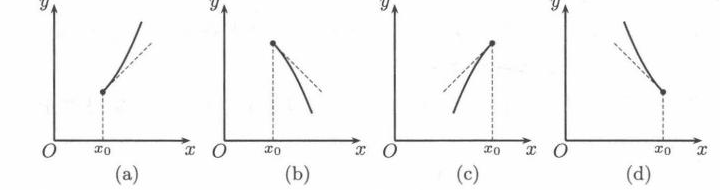
\includegraphics[width=.82\linewidth]{figures/upper/ch07/fig-7-1.png}

  图 7.1
\end{center}

下面给出 Fermat 定理的两个证明。第一个证明以命题 7.1.1 为依据，第二个证明则完全不同，它是用上一章的无穷小增量公式为工具。

\begin{xproposition}[7.1.2（Fermat 定理）]
若 $x_0$ 是函数 $f$ 的极值点，且存在导数 $f'(x_0)$，则一定有 $f'(x_0)=0$。
\end{xproposition}
\begin{xproof}
\textbf{证 1}\quad 不妨只给出 $x_0$ 为极小值点时的证明。根据定义，存在 $\delta>0$，使得当 $\abs{x-x_0}<\delta$ 时，成立
\begin{equation}
  f(x)\geqslant f(x_0).
  \tag{7.1}
\end{equation}
由于存在导数 $f'(x_0)$，所以两个单侧导数存在且相等，即有
\begin{equation}
  f'(x_0)=f'_-(x_0)=f'_+(x_0).
  \tag{7.2}
\end{equation}
从命题 7.1.1 之 (2) 和它对于 $f'_-(x_0)$ 的平行结论，就有
\[
  f'_+(x_0)\geqslant0,\qquad f'_-(x_0)\leqslant0.
\]
与 (7.2) 合并，就得到 $f'(x_0)=0$。

\textbf{证 2}\quad 利用无穷小增量公式 (6.1)，可以写出
\[
  \begin{aligned}
    f(x)-f(x_0)&=f'(x_0)(x-x_0)+\littleo(x-x_0)\quad(x\to x_0)\\
    &=[f'(x_0)+\littleo(1)](x-x_0)\quad(x\to x_0).
  \end{aligned}
\]
用反证法：若 $f'(x_0)\neq0$，则当 $x$ 与 $x_0$ 充分接近时，$[f'(x_0)+\littleo(1)]$ 与 $f'(x_0)$ 同号，因此当变量 $x$ 经过 $x_0$ 时，$f(x)-f(x_0)$ 变号。这与 $x_0$ 为极值点矛盾。
\end{xproof}

\begin{xremark}
以上两个证明方法都很重要。第一个证明的主要工具（即命题 7.1.1）还会出现在下面的命题 7.1.6（Darboux 定理）的证明中。第二个证明的方法可用于处理更为一般的极值条件（见例题 8.3.1）。
\end{xremark}

\begin{xremark}
由 Fermat 定理知道，若 $x_0$ 是 $f(x)$ 的极值点，则只有两种情况：(1) $f(x)$ 在点 $x_0$ 处不可导；(2) $f'(x_0)$ 存在且等于零。因此在寻找函数 $f$ 的极值点时，将 $f$ 的不可导点和导数为零的点统称为“极值可疑点”。当然这只是“可疑”，因为容易举例说明 $f$ 在点 $x_0$ 不可导或 $f'(x_0)=0$ 时，$f(x)$ 并不一定在点 $x_0$ 处达到极值。
\end{xremark}

\begin{xremark}
若 $f'(x_0)=0$，则称 $x_0$ 为\textbf{驻点}（stationary point），或\textbf{平稳点}。这些名字的意思是说在这种点的附近，因变量 $f(x)$ 的值几乎不变。确切地说，从无穷小增量公式 (6.1) 和条件 $f'(x_0)=0$ 就可得出
\[
  \Delta y=f(x)-f(x_0)=\littleo(\Delta x)\quad(\Delta x\to0).
\]
即当 $\Delta x\to0$ 时，$\Delta y$ 是 $\Delta x$ 的高阶无穷小。不妨看一个具体例子来理解这是什么意思。设 $y=x^3+1$，则 $x_0=0$ 是驻点，$y(0)=1$。当 $x=0.1$ 时，$y=1.001$，而当 $x=0.01$ 时，$y=1.000\,001$。
\end{xremark}

第二个基本定理是 Rolle 定理，也可称为 Rolle 中值定理。

\begin{xproposition}[7.1.3（Rolle 定理）]
设 $f$ 在 $[a,b]$ 上连续，在 $(a,b)$ 上可微，且有 $f(a)=f(b)$，则存在 $\xi\in(a,b)$，使得 $f'(\xi)=0$。
\end{xproposition}
\begin{xproof}
\textbf{证 1}\quad 若 $f$ 是区间 $[a,b]$ 上的常值函数，则在 $(a,b)$ 的每一点上有 $f'(x)=0$。因此可以在 $(a,b)$ 中任取一点作为 $\xi$。

否则，由有界闭区间上连续函数的值域定理知，$f$ 在 $[a,b]$ 上取到自己的最大值 $M$ 和最小值 $m$，且有 $m<M$。由于有题设条件 $f(a)=f(b)$，因此在 $m$ 和 $M$ 中，至少有一个与函数在端点的值不同。这就是说，至少有一个最值是在 $(a,b)$ 中取到的。设这个最值点为 $\xi\in(a,b)$。由于在区间的内点处取到的最值也就是极值，而函数 $f$ 又在 $(a,b)$ 上可微，因此可以用 Fermat 定理，知道 $f'(\xi)=0$。
\end{xproof}

\begin{xremark}
我们看到，Fermat 定理的证明只需要很少的函数极限知识，但是在 Rolle 定理的证明中则需要用连续函数的一个基本定理——最值定理。回忆这个基本定理的证明方法，以及它所涉及的许多知识，可以知道 Rolle 定理看似容易，实际上是前面许多内容的结晶。而这还是刚刚开始。下面的其他许多结果都是直接或间接地建筑在 Rolle 定理的基础之上的。
\end{xremark}

\begin{xremark}
在 Rolle 定理的三个条件中任意去掉一个或几个，定理的结论就不再成立。这些训练对于理解 Rolle 定理很有必要，在一般教科书中也都有，这里不再重复。
\end{xremark}

\begin{xremark}
Rolle 定理的上述证明即是一般教科书均采用的经典证明。它以闭区间上连续函数的最值定理和 Fermat 定理为主要工具。但是实际上 Rolle 定理和这两个定理并无必然联系。将这一点再延伸一步就可以说，本章从 Rolle 定理开始的全部内容都无须用 Fermat 定理就可以建立起来。支持上述观点的根据就是 Rolle 定理的新证明，其中所用的工具是连续函数的零点存在定理和闭区间套定理（见《美国数学月刊》(1979) 第 86 卷 484--486 页）。此外还有用覆盖定理和 Dedekind 定理证明 Rolle 定理的工作（参见 [57]）。
\end{xremark}

\paragraph{证 2（Rolle 定理的 Samuleson（萨缪尔森）证明）}
作辅助函数
\[
  F(x)=f(x)-f\left(x+\frac{b-a}{2}\right),\qquad a\leqslant x\leqslant\frac{a+b}{2}.
\]
则可以从条件 $f(a)=f(b)$ 得出
\[
  F(a)=f(a)-f\left(\frac{a+b}{2}\right),\qquad
  F\left(\frac{a+b}{2}\right)=f\left(\frac{a+b}{2}\right)-f(b)=-F(a).
\]
在区间 $\left[a,\frac12(a+b)\right]$ 上对函数 $F$ 用零点存在定理，知道存在 $a_1\in\left[a,\frac12(a+b)\right]$，使得 $F(a_1)=0$。记 $b_1=a_1+\frac12(b-a)$，则就有（见图 7.2）
\[
  f(a_1)=f(b_1),\qquad [a_1,b_1]\subset[a,b],\qquad b_1-a_1=\frac12(b-a).
\]
将以上做法继续下去，得到一个闭区间套 $\{[a_n,b_n]\}$，它满足要求：
\[
  b_n-a_n=\frac{1}{2^n}(b-a),\qquad f(a_n)=f(b_n),\qquad n\in\NN_+.
\]
应用闭区间套定理，存在唯一的点 $\xi$，它属于每个闭区间 $[a_n,b_n]$，也就是说有不等式
\begin{equation}
  a_n\leqslant\xi\leqslant b_n,\qquad \forall n\in\NN_+.
  \tag{7.3}
\end{equation}
而且有
\begin{equation}
  \lim_{n\to\infty}a_n=\lim_{n\to\infty}b_n=\xi.
  \tag{7.4}
\end{equation}
这里需要补充一点，即总可以使得 $\xi\in(a,b)$。为此只要使得 $\{a_n\}$ 和 $\{b_n\}$ 不是常值数列就可以了。实际上，若有 $a=a_1=a_2$，则
\[
  f(a)=f(a_1)=f(a_2)=f(b_1)=f(b_2),
\]
可用 $[b_2,b_1]$ 代替 $[a_2,b_2]$ 进行下去。同样可以避免 $\{b_n\}$ 为常值数列。

由于 $f$ 在点 $\xi\in(a,b)$ 可导，因此就有
\begin{equation}
  \lim_{n\to\infty}\frac{f(b_n)-f(a_n)}{b_n-a_n}=f'(\xi).
  \tag{7.5}
\end{equation}
为此只要写出无穷小增量公式：
\[
  f(b_n)=f(\xi)+f'(\xi)(b_n-\xi)+\littleo(b_n-\xi)\quad(b_n\to\xi),
\]
\[
  f(a_n)=f(\xi)+f'(\xi)(a_n-\xi)+\littleo(a_n-\xi)\quad(a_n\to\xi),
\]
代入 (7.5) 左边的分子，并利用 (7.3) 和 (7.4) 即可。

由于 $f(a_n)=f(b_n),\ \forall n\in\NN_+$，因此从 (7.5) 可见 $f'(\xi)=0$。

\begin{xremark}
以上证明的基本思想有两点。(1) 第一步是用 $a_1,b_1$ 代替原来的区间端点 $a$ 和 $b$，一方面保持了在两个点上的函数值相等，另一方面则使两点之间的距离缩小了一半。（关于这一步可以参考第五章第一组参考题 2 的内容。）以下就是不断重复，用闭区间套定理得到唯一的点 $\xi$。(2) 利用极限 (7.5)，就保证得到 $f'(\xi)=0$。在图 7.2 中我们显示了构造闭区间套过程的开始几步，即有 $f(a_1)=f(b_1),\ b_1-a_1=\frac12(b-a)$，$f(a_2)=f(b_2),\ b_2-a_2=\frac12(b_1-a_1)$。在图 7.2 上似乎最后得到的点 $\xi$ 是 $f$ 的极值点。但实际上可以举出例子，使得在 Samuleson 证明中得到的 $\xi$ 可以不是极值点（作为\textbf{思考题}）。因此这个证明与前面的经典证明确实是完全不同的。
\end{xremark}

\begin{center}
  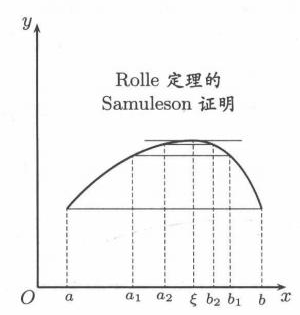
\includegraphics[width=.40\linewidth]{figures/upper/ch07/fig-7-2.png}

  图 7.2
\end{center}

将 Rolle 定理中的条件 $f(a)=f(b)$ 去掉后加以推广，就得到下面的 Lagrange 中值定理。虽然可以说 Rolle 定理更为基本，但总的来说 Lagrange 中值定理的用处要大得多，因为它很好地解决了函数研究中的一个基本问题——如何将自变量从 $a$ 到 $b$ 时所引起的因变量的增量与导数联系起来。从 Lagrange 中值定理的内容来说，也已经包含了 Rolle 定理为其特例。以下采用与多数教科书中的经典证明不同的面积证明方法。

\begin{xproposition}[7.1.4（Lagrange 中值定理）]
设 $f$ 在 $[a,b]$ 上连续，在 $(a,b)$ 上可微，则存在 $\xi\in(a,b)$，使得
\[
  f'(\xi)=\frac{f(b)-f(a)}{b-a}.
\]
\end{xproposition}

\paragraph{分析}
先在图 7.3 中的 $f$ 的图像上任取一点 $(x,f(x))$，然后将它同点 $(a,f(a))$，$(b,f(b))$ 连接成一个三角形（图中阴影区）。记它的面积为 $S(x)$。如果让这个三角形的顶点 $(x,f(x))$ 平行它的对边移动（见图 7.3 经过该点的一条直线），则三角形面积不变。这条对边就是连接 $(a,f(a))$ 和 $(b,f(b))$ 的直线段。由此可见，如果 $\xi$ 是函数 $S(x)$ 的驻点（见 Fermat 定理证明后的注解 3），则 $f$ 的图像在点 $(\xi,f(\xi))$ 的切线就可能同这条直线段平行。而这就是定理中对点 $\xi$ 的要求。根据这个几何分析就可以写出以下证明。

\begin{center}
  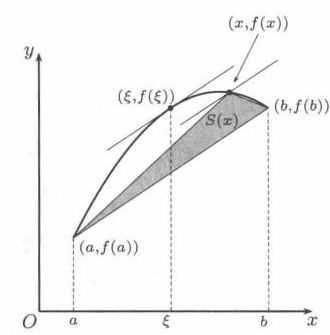
\includegraphics[width=.42\linewidth]{figures/upper/ch07/fig-7-3.png}

  图 7.3
\end{center}

\begin{xproof}
Lagrange 中值定理的面积证明。用行列式构造辅助函数：
\begin{equation}
  \Delta(x)=
  \begin{vmatrix}
    1&1&1\\
    a&b&x\\
    f(a)&f(b)&f(x)
  \end{vmatrix}
  =
  \begin{vmatrix}
    b-a&x-a\\
    f(b)-f(a)&f(x)-f(a)
  \end{vmatrix}.
  \tag{7.6}
\end{equation}
（这个 $\Delta(x)$ 的值等于图 7.3 中的三角形面积 $S(x)$ 的两倍。）利用 $\Delta(a)=\Delta(b)=0$，从 Rolle 定理知道有 $\xi\in(a,b)$，使得 $\Delta'(\xi)=0$。写出
\[
  \Delta'(x)=
  \begin{vmatrix}
    1&1&0\\
    a&b&1\\
    f(a)&f(b)&f'(x)
  \end{vmatrix}
  =
  \begin{vmatrix}
    b-a&1\\
    f(b)-f(a)&f'(x)
  \end{vmatrix},
\]
就可以从 $\Delta'(\xi)=0$ 直接得到所要求证的结论。
\end{xproof}

\begin{xremark}
Rolle 定理和 Lagrange 中值定理都具有清晰的几何意义。在图 7.3 中作出了曲线 $y=f(x)$ 在点 $(\xi,f(\xi))$ 处的切线，它与连接点 $(a,f(a))$ 和 $(b,f(b))$ 的直线段平行。Lagrange 中值定理的经典证明就是从这个几何意义出发，将 $f$ 的图像“减去”上述直线段来构造辅助函数。由于一般教科书中均用这个证明，本书不再重复。上面的面积证明也是以几何背景为出发点的，同时还利用了驻点所具有的特性。又由于三角形面积可以用行列式表示，从而证明过程带有更多的代数色彩。这种证明方法还可以用于证明下面的 Cauchy 中值定理（留作\textbf{思考题}）。

应当看到，几何作图虽然很有用，但每张图都有局限性。例如，图 7.2 和 7.3 似乎提示我们中值 $\xi$ 是唯一的。实际上不一定如此。中值可以有多个，甚至无穷多个。此外，今后所遇到的许多问题并不一定都有几何背景。即使确实有几何背景，也不一定明显。因此我们在下面将介绍构造辅助函数的其他方法，它在许多问题中更实用一些。
\end{xremark}

\begin{xremark}
也可以从物理上来理解这两个定理的意义。例如，设自变量 $x$ 为时间，因变量 $y$ 是质点做直线运动时从某点起算的路程，将 $a$ 和 $b$ 作为时间的起点和终点。Rolle 定理表明，若质点在起点和终点的位置相同，则一定有瞬时速度为零的时刻。这个时刻在 Rolle 定理的（第一个）证明中就是质点运动转向的时刻。同样，Lagrange 中值定理的运动学意义也很清楚。它表明一定存在一个时刻 $\xi$，使得在该时刻的瞬时速度恰好是质点运动（从时刻 $a$ 到 $b$）的平均速度。
\end{xremark}

\begin{xremark}
Lagrange 中值定理有下列各种形式，经常称为\textbf{有限增量公式}：
\begin{align}
  f(b)&=f(a)+f'(\xi)(b-a),\qquad a<\xi<b, \tag{7.7}\\
  f(b)&=f(a)+f'(a+\theta(b-a))(b-a),\qquad 0<\theta<1, \tag{7.8}\\
  \Delta y&=f'(x_0+\theta\Delta x)\Delta x,\qquad 0<\theta<1. \tag{7.9}
\end{align}
将它们与上一章中的无穷小增量公式 (6.1) 或 (6.3) 作比较，就可以看出这里已经前进了一大步。从今以后，我们有了与过去完全不同的有力工具，在本章以及今后所能解决的许多问题都是过去的“原始”工具所难以对付的。
\end{xremark}

\begin{xremark}
Lagrange 中值定理将函数的增量与函数在一个点上的导数值联系起来，这就为用微分学研究函数提供了基础。希望读者从今后的大量实例中体会引进导数（即变化率）的重要性。
\end{xremark}

本节的最后一个定理是

\begin{xproposition}[7.1.5（Cauchy 中值定理）]
设函数 $f,g$ 在 $[a,b]$ 上连续，在 $(a,b)$ 上可微，且满足条件
\[
  g(b)-g(a)\neq0\quad\text{和}\quad f'^2(x)+g'^2(x)\neq0,\qquad \forall x\in(a,b),
\]
则存在 $\xi\in(a,b)$，使得
\[
  \frac{f(b)-f(a)}{g(b)-g(a)}=\frac{f'(\xi)}{g'(\xi)}.
\]
\end{xproposition}

\begin{xproof}
引进记号
\[
  \lambda=\frac{f(b)-f(a)}{g(b)-g(a)}.
\]
我们的目的是要证明存在 $\xi\in(a,b)$，使得
\begin{equation}
  f'(\xi)-\lambda g'(\xi)=0.
  \tag{7.10}
\end{equation}
这里要说明，如有 $g'(\xi)=0$，则由上式可见也有 $f'(\xi)=0$，这与条件 $f'^2(x)+g'^2(x)\neq0,\ \forall x\in(a,b)$ 相矛盾。因此有了 (7.10) 之后，就一定有 $g'(\xi)\neq0$，从而可以由它推出定理中所要的等式。

由 (7.10) 出发试作辅助函数
\[
  F(x)=f(x)-\lambda g(x).
\]
然后计算
\[
  F(a)=f(a)-\frac{f(b)-f(a)}{g(b)-g(a)}\cdot g(a)
      =\frac{f(a)g(b)-f(b)g(a)}{g(b)-g(a)},
\]
\[
  F(b)=f(b)-\frac{f(b)-f(a)}{g(b)-g(a)}\cdot g(b)
      =\frac{f(a)g(b)-f(b)g(a)}{g(b)-g(a)},
\]
可见有 $F(a)=F(b)$。然后对 $F(x)$ 在区间 $[a,b]$ 上应用 Rolle 定理，就知道存在 $\xi\in(a,b)$，使得 $F'(\xi)=0$。这就是要证明的结果 (7.10)。
\end{xproof}

\begin{xremark}
容易看出，只要 $g(x)=x$，就从 Cauchy 中值定理得到 Lagrange 中值定理。因此 Cauchy 中值定理是 Lagrange 中值定理的一种推广。由于它能同时处理两个函数，因此在今后的许多问题中起重要作用。
\end{xremark}

\begin{xremark}
与 Rolle 定理和 Lagrange 中值定理一样，Cauchy 中值定理也有漂亮的几何意义。为此可以先将定理中的自变量改记为 $t$，然后用参数方程
\[
  x=g(t),\qquad y=f(t)
\]
定义在平面上的一条曲线。如图 7.4 所示，该曲线的两个端点是 $(g(a),f(a))$ 和 $(g(b),f(b))$。定理中关于两个函数 $f,g$ 在 $[a,b]$ 上连续和在 $(a,b)$ 上可微的条件表明，这条曲线不但连续，而且在（除去端点之外的）每一点都有切线。实际上从参数方程的求导法则（命题 6.2.1）知道，当 $g'(t)\neq0$ 时，切线的斜率
\[
  \frac{\dd y}{\dd x}=\frac{f'(t)}{g'(t)}
\]
是有限数。同样可以知道，当 $g'(t)=0$ 但 $f'(t)\neq0$ 时，切线将平行于 $y$ 轴。在 Cauchy 中值定理中的另一个条件 $g(b)-g(a)\neq0$ 表明，连接曲线两个端点的直线段不平行于 $y$ 轴，因此它的斜率
\[
  \frac{f(b)-f(a)}{g(b)-g(a)}
\]
是有限数。这样一来就可以看出，Cauchy 中值定理的结论就是说（至少）存在一个参数值 $\xi\in(a,b)$，使得在曲线上的点 $(g(\xi),f(\xi))$ 的切线恰好与连接曲线两个端点 $(g(a),f(a))$ 和 $(g(b),f(b))$ 的直线段平行。
\end{xremark}

\begin{center}
  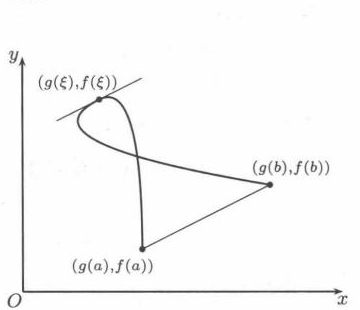
\includegraphics[width=.40\linewidth]{figures/upper/ch07/fig-7-4.png}

  图 7.4
\end{center}

\begin{xremark}
如果在 Cauchy 中值定理中的条件修改为 $g'(x)\neq0,\ \forall x\in(a,b)$，则可以用 $g(x)$ 的反函数为工具，从 Lagrange 中值定理推出 Cauchy 中值定理。由于这个条件对于用参数方程给出的曲线增加了不必要的限制，排除了例如图 7.4 中那样的曲线，因此本书采用了较一般的条件。从图中可以看出，曲线上某些点处的切线可以与 $y$ 轴平行，曲线也可以有自交点，Cauchy 中值定理仍然成立。
\end{xremark}

\begin{xremark}
如果在某点 $t_0\in(a,b)$ 发生 $f'(t_0)=g'(t_0)=0$，则称点 $(f(t_0),g(t_0))$ 为曲线 $x=f(t),y=g(t)$ 的\textbf{奇点}。奇点有几种不同的类型。本书中将在第八章的例题 8.6.1 中介绍奇点中的“尖点”（见图 8.10）。
\end{xremark}

\subsection{导函数的两个定理}

本小节证明关于导函数的两个基本定理。第一个定理（Darboux 定理）是说区间上的导函数一定具有介值性质，即使导函数不连续时也如此。第二个定理称为单侧导数极限定理或导数极限定理，由此可以推出导函数不会有第一类间断点。这两个定理都表明导函数具有特殊性质。因此并不是每个函数都可以是某个函数的导函数。这两个定理在今后，特别是在积分学中，要起重要作用。

\begin{xproposition}[7.1.6（Darboux 定理）]
设 $f$ 在区间 $I$ 上可微，则 $f'$ 具有介值性质。
\end{xproposition}

首先说明定理的意义。在第五章中我们已经有连续函数的介值定理（即命题 5.2.2）。如果导函数 $f'\in C(I)$，则已不必再讨论。可见本命题的意义在于，区间上的导函数不论是否连续，一定有介值性质。

\begin{xproof}
\textbf{证 1}\quad （这是多数教科书中采用的经典证明。这里只作简述。需要了解细节的读者可参考 [14] 第一卷的 110 小节。）

仿照 §5.2，分两步进行。

(1) 为确定起见，不妨设有 $a,b\in I,\ a<b$，使得 $f'(a)<0,\ f'(b)>0$。如图 7.5 所示，应用命题 7.1.1 知道存在 $\delta>0$，使得成立 $a+\delta<b-\delta$，且满足
\begin{equation}
  f(a+\delta)<f(a),\qquad f(b-\delta)<f(b).
  \tag{7.11}
\end{equation}
因此在 $[a,b]$ 上 $f$ 的最小值点 $\xi$ 一定是内点，即极小值点。应用 Fermat 定理就得到 $f'(\xi)=0$。

(2) 对于 $f'(a)\neq f'(b)$ 的一般情况。为确定起见，不妨设有 $f'(a)<c<f'(b)$。构造辅助函数
\[
  F(x)=f(x)-cx.
\]
就可以将问题归结为 (1) 而知道 $f'$ 能取到 $c$（细节从略）。

\textbf{证 2}\quad 与 Rolle 定理的 Samuleson 证明类似，Darboux 定理的证明并不一定要用 Fermat 定理。当然只需要修改证明 1 中的第 (1) 步。若有 $f(a)=f(b)$，则用 Rolle 定理即可。否则，不妨只看 $f(a)>f(b)$ 的情况（见图 7.5）。由于有 $\delta>0$，使得 $f(a)>f(b)>f(b-\delta)$，应用连续函数的介值定理，就知道存在 $\eta\in(a,b-\delta)$，满足 $f(\eta)=f(b)$。在 $[\eta,b]$ 上再用 Rolle 定理即可（见图 7.5）。
\end{xproof}

\begin{center}
  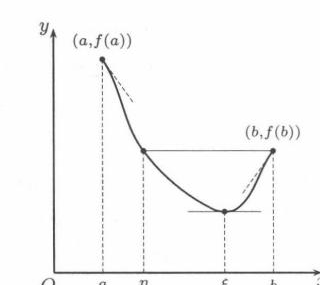
\includegraphics[width=.38\linewidth]{figures/upper/ch07/fig-7-5.png}

  图 7.5
\end{center}

在上一章关于导数概念的讨论中，我们曾强调过不要混淆函数在某点的单侧导数和这个函数的导函数在该点同侧的单侧极限。这是两个不同的概念。但是在那里还没有条件提及事情的另一方面，即实际上这两者的值在很多情况中确实相等。例题 6.1.6 就是如此。这里的规律性就是下一个命题的内容。根据这个命题，今后对例题 6.1.6 类型的题可以有新的做法。

\begin{xproposition}[7.1.7（单侧导数极限定理）]
设在区间 $[a,b]$ 上有定义的函数 $f$ 在 $(a,b)$ 上可微，又在点 $a$ 右连续。若导函数 $f'(x)$ 在点 $a$ 存在右侧极限 $f'(a+)=A$，则 $f$ 在点 $a$ 也一定存在右侧导数 $f'_+(a)$，且成立
\[
  f'_+(a)=f'(a+)=A,
\]
即 $f'(x)$ 在点 $a$ 右连续。此外，这里的 $A$ 除了为有限数外，也可以为 $\pm\infty$。
\end{xproposition}

\begin{xproof}
令 $\Delta x=x-a,\ \Delta y=f(x)-f(a)$，写出函数 $f$ 在点 $a$ 右侧的差商
\[
  \frac{\Delta y}{\Delta x}=\frac{f(a+\Delta x)-f(a)}{\Delta x},\qquad \Delta x>0.
\]
在闭区间 $[a,a+\Delta x]$ 上应用 Lagrange 中值定理 (7.9)，有 $0<\theta<1$，使得
\[
  \Delta y=f(a+\Delta x)-f(a)=f'(a+\theta\Delta x)\Delta x.
\]
因此在 $\Delta x>0$ 时就有
\[
  \frac{\Delta y}{\Delta x}=f'(a+\theta\Delta x).
\]
现设有 $\lim_{x\to a+}f'(x)=A$，其中 $A$ 为有限数。则对 $\varepsilon>0$，存在 $\delta>0$，使得当 $a<x<a+\delta$ 时，成立不等式
\[
  \abs{f'(x)-A}<\varepsilon.
\]
若有 $0<\Delta x=x-a<\delta$，则同时就有 $a<a+\theta\Delta x<x<a+\delta$。因此当 $0<\Delta x<\delta$ 时，也就有
\[
  \abs{\frac{\Delta y}{\Delta x}-A}=\abs{f'(a+\theta\Delta x)-A}<\varepsilon.
\]
这样就证明了函数 $f$ 在点 $a$ 存在右侧导数，且等于 $A$。对于 $A$ 不是有限数的情况，证明类似，请读者补全。
\end{xproof}

对于下列问题，如果肯定，请作出证明；如果否定，请举出例子。

\begin{xthought}[1]
如果在命题中将函数 $f$ 在点 $a$ 右连续的条件去掉，则结论是否还能成立？
\end{xthought}
\begin{xsolution}
可以构造一个很简单的例子。于 $[-1,1]$ 上定义
\[
  f(x)=
  \begin{cases}
    x^2\sin\dfrac{\pi}{x},&x\neq0,\\
    0,&x=0.
  \end{cases}
\]
函数 $f$ 连续，并且
\[
  f'(0)=\lim_{x\to0}x\sin\frac{\pi}{x}=0.
\]
对 $m=0,1,2,\ldots$ 取
\[
  [a_m,b_m]=[-2^{-m},2^{-m}].
\]
由于
\[
  f(\pm2^{-m})=0,
  \qquad
  b_{m+1}-a_{m+1}=\frac12(b_m-a_m),
\]
这些区间可以作为 Samuleson 构造中的闭区间套，其唯一公共点为 $\xi=0$。

但是 $0$ 不是极值点。例如对 $m=1,2,\ldots$ 令
\[
  x_m=\frac{1}{2m+\frac12},
  \qquad
  y_m=\frac{1}{2m+\frac32},
\]
则 $x_m,y_m\to0+$，且
\[
  f(x_m)=x_m^2>0,
  \qquad
  f(y_m)=-y_m^2<0.
\]
故 $f$ 在 $0$ 的任意邻域内都同时取正值和负值。于是 Samuleson 证明得到的 $\xi$ 确实不必是极值点。

否。右连续条件不能删去。取 $a=0$，并在 $[0,1]$ 上定义
\[
  f(0)=1,
  \qquad
  f(x)=0\quad(0<x\leqslant1).
\]
则在 $(0,1)$ 上 $f'(x)=0$，所以
\[
  \lim_{x\to0+}f'(x)=0.
\]
但
\[
  \frac{f(x)-f(0)}x=-\frac1x\to-\infty,
\]
故 $f'_+(0)$ 不等于上述导函数极限。这里失败的原因正是 $f$ 在 $0$ 不右连续。
\end{xsolution}


\begin{xthought}[2]
如果命题中的 $A$ 是无穷大量，而且不具有确定的符号，则结论是否还能成立？
\end{xthought}
\begin{xsolution}
仿照 Lagrange 中值定理的面积证明，定义
\[
  \Delta(t)=
  \begin{vmatrix}
    1&1&1\\
    g(a)&g(b)&g(t)\\
    f(a)&f(b)&f(t)
  \end{vmatrix}.
\]
显然 $\Delta(a)=\Delta(b)=0$。由 Rolle 定理，存在 $\xi\in(a,b)$ 使 $\Delta'(\xi)=0$。直接求导得
\[
  0=\Delta'(\xi)
  =
  \begin{vmatrix}
    g(b)-g(a)&g'(\xi)\\
    f(b)-f(a)&f'(\xi)
  \end{vmatrix},
\]
即
\[
  [g(b)-g(a)]f'(\xi)-[f(b)-f(a)]g'(\xi)=0.
\]
若 $g'(\xi)=0$，由 $g(b)-g(a)\neq0$ 可推出 $f'(\xi)=0$，这与
\[
  f'^2(\xi)+g'^2(\xi)\neq0
\]
矛盾。因此 $g'(\xi)\neq0$，从而
\[
  \frac{f(b)-f(a)}{g(b)-g(a)}
  =\frac{f'(\xi)}{g'(\xi)}.
\]
这就是 Cauchy 中值定理。

否。取 $a=0$，并在 $[0,1]$ 上定义
\[
  f(0)=0,
  \qquad
  f(x)=x^2\sin\frac1{x^2}\quad(x>0).
\]
则 $f$ 在 $0$ 右连续，而且
\[
  f'_+(0)=\lim_{x\to0+}\frac{f(x)-f(0)}x
  =\lim_{x\to0+}x\sin\frac1{x^2}=0.
\]
另一方面，当 $x>0$ 时
\[
  f'(x)=2x\sin\frac1{x^2}-\frac2x\cos\frac1{x^2}.
\]
取
\[
  x_n=\frac1{\sqrt{2n\pi}},
  \qquad
  y_n=\frac1{\sqrt{(2n+1)\pi}},
\]
则 $x_n,y_n\to0+$，并且
\[
  f'(x_n)=-\frac2{x_n}\to-\infty,
  \qquad
  f'(y_n)=\frac2{y_n}\to+\infty.
\]
因此 $f'(x)$ 在 $0$ 的右侧是无界且无确定符号的，但 $f'_+(0)$ 却存在并等于 $0$。所以把命题中的 $A$ 放宽为这种“无确定符号的无穷大量”后，原结论不再成立。
\end{xsolution}


\begin{xthought}[3]
如果存在 $f'_+(a)=A$，则是否存在 $f'(a+)$？为什么？
\end{xthought}
\begin{xsolution}
否。取
\[
  f(0)=0,
  \qquad
  f(x)=x^2\sin\frac1x\quad(x\neq0).
\]
则
\[
  f'_+(0)=\lim_{x\to0+}x\sin\frac1x=0.
\]
但对 $x\neq0$，
\[
  f'(x)=2x\sin\frac1x-\cos\frac1x,
\]
当 $x\to0+$ 时没有极限。因此 $f'_+(a)$ 存在并不能推出 $f'(a+)$ 存在。
\end{xsolution}


若不只是考虑单侧情况，就可以得到

\begin{xtheorem}[导数极限定理]
设函数 $f$ 在点 $a$ 的某邻域 $O(a)$ 上连续，在 $O(a)-\{a\}$ 上可导。若 $f'$ 在点 $a$ 处存在极限，则 $f$ 在点 $a$ 处也可导，而且 $f'$ 在点 $a$ 处连续。
\end{xtheorem}

\begin{xremark}
由此可见，若导函数在某点有极限，则它就在该点连续。这里甚至事先不要假定函数在该点可导。回顾一般函数在某点存在极限时可以在该点不连续，可见导函数的这个性质也是很独特的。
\end{xremark}

\begin{xexample}[7.1.1]
设 $f$ 在区间 $(a,b)$ 上可微，则导函数 $f'(x)$ 不会有第一类间断点。
\end{xexample}
\begin{xproof}
用反证法：设点 $c\in(a,b)$ 是 $f'(x)$ 的第一类间断点，则导函数 $f'$ 在点 $c$ 存在有限的两个单侧极限
\[
  f'(c-)\quad\text{和}\quad f'(c+).
\]
又因存在 $f'(c)$，所以 $f$ 在 $c$ 连续，这包含了函数 $f$ 在该点的两个单侧连续性。

应用命题 7.1.7 的结论，知道成立两个等式：
\[
  f'(c-)=f'_-(c)\quad\text{和}\quad f'(c+)=f'_+(c).
\]
由于 $f$ 在 $c$ 可导，因此有
\[
  f'_-(c)=f'(c)=f'_+(c).
\]
合并这些结果就得到
\[
  f'(c-)=f'(c)=f'(c+).
\]
这恰恰表明导函数 $f'(x)$ 在点 $c$ 连续。引出矛盾。
\end{xproof}

\begin{xremark}
在区间上的导函数可以有第二类间断点，见例题 6.1.5 及其图 6.3。
\end{xremark}

\subsection{例题}

由于本章的以下内容和下一章的大多数内容都可以说是中值定理的应用，因此例题极多，举不胜举。凡能列入其他章节中的例题均不放在这一小节。

从 Rolle 定理知道，可微函数的两个零点之间一定有导函数的零点。以下举一个这方面的例题。初学者需要通过习题来熟悉这种基本方法。

\begin{xexample}[7.1.2]
设
\[
  \frac{a_0}{n+1}+\frac{a_1}{n}+\cdots+a_n=0,
\]
证明：方程
\[
  f(x)=a_0x^n+a_1x^{n-1}+\cdots+a_n=0
\]
在区间 $(0,1)$ 中至少有一个根。
\end{xexample}
\begin{xproof}
构造辅助函数
\[
  F(x)=\frac{a_0x^{n+1}}{n+1}+\frac{a_1x^n}{n}+\cdots+a_nx,
\]
则可见 $F(0)=F(1)=0$。对 $F$ 在区间 $[0,1]$ 上用 Rolle 定理，就知道 $F'(x)=f(x)$ 在区间 $(0,1)$ 中有零点。
\end{xproof}

\begin{xexample}[7.1.3]
设 $f$ 在 $[a,b]$ 上二阶可微，$f(a)=f(b)=0$。证明：对每个 $x\in(a,b)$，存在 $\xi\in(a,b)$，使得成立
\[
  f(x)=\frac{f''(\xi)}{2}(x-a)(x-b).
\]
\end{xexample}
\begin{xproof}
\textbf{证 1}\quad 固定 $x\in(a,b)$，令
\[
  \lambda=\frac{2f(x)}{(x-a)(x-b)}.
\]
于是只要证明存在 $\xi\in(a,b)$，使成立 $f''(\xi)=\lambda$。构造在 $[a,b]$ 上的辅助函数
\[
  F(t)=f(t)-\frac{\lambda}{2}(t-a)(t-b).
\]
由条件 $f(a)=f(b)=0$ 得到 $F(a)=F(b)=0$。从 $\lambda$ 的定义又还可得到 $F(x)=0$。在区间 $[a,x]$ 和 $[x,b]$ 上分别对 $F$ 用 Rolle 定理得到两个点 $\eta_1$ 和 $\eta_2$，满足条件
\[
  a<\eta_1<x<\eta_2<b\quad\text{和}\quad F'(\eta_1)=F'(\eta_2)=0.
\]
然后再在区间 $[\eta_1,\eta_2]$ 上对 $F'$ 用 Rolle 定理，知道有 $\xi\in(\eta_1,\eta_2)\subset(a,b)$，满足要求 $F''(\xi)=0$。这就是 $f''(\xi)=\lambda$。

\textbf{证 2}\quad 也可以用 Cauchy 中值定理来证明。将要证明的等式改写为
\begin{equation}
  f''(\xi)=\frac{2f(x)}{(x-a)(x-b)}.
  \tag{7.12}
\end{equation}
记区间 $[a,b]$ 的中点为 $c=\frac12(a+b)$。若 $f'(c)\neq0$，则在 (7.12) 右边的分子和分母中将 $x$ 换为变量 $t$ 后得到的一对函数的导数不会同时为 0，因此可利用条件 $f(a)=f(b)=0$，在子区间 $[a,x]$ 和 $[x,b]$ 上分别用 Cauchy 中值定理得到
\[
  \frac{2f(x)}{(x-a)(x-b)}
  =\frac{f'(\eta_1)}{\eta_1-c}
  =\frac{f'(\eta_2)}{\eta_2-c}
  =\frac{f'(\eta_1)-f'(\eta_2)}{\eta_1-\eta_2},
\]
其中 $\eta_1$ 和 $\eta_2$ 满足要求 $a<\eta_1<x<\eta_2<b$。最后再用 Lagrange 中值定理，得到 $\xi\in(\eta_1,\eta_2)$，使 (7.12) 成立。

若有 $f'(c)=0$，则对于每个 $x\in(a,b)$，在子区间 $[a,x]$ 和 $[x,b]$ 中至少有一个子区间上仍可用 Cauchy 中值定理，并计算如下：
\[
  \frac{2f(x)}{(x-a)(x-b)}
  =\frac{f'(\eta)}{\eta-c}
  =\frac{f'(\eta)-f'(c)}{\eta-c}
  =f''(\xi).
\]
\end{xproof}

\begin{xremark}
以上两种方法可以解决许多类似的问题。实际上如果仔细分析的话，容易发现这两个方法并无多大差别。只不过在写法上略有不同而已。其中第一个方法可以称为特定\textbf{常数法}，是作辅助函数的一种很有用的方法。
\end{xremark}

在某些情况下，我们可能对中值定理中的中值 $\xi$ 有进一步的了解。

\begin{xexample}[7.1.4]
设函数 $f$ 在点 $a$ 处二阶可导，且 $f''(a)\neq0$，则在 $h$ 充分小时，成立
\[
  f(a+h)-f(a)=f'(a+\theta h)h,
\]
而且其中的 $\theta$ 具有性质 $\lim_{h\to0}\theta(h)=1/2$。
\end{xexample}
\begin{xproof}
由于存在 $f''(a)$，因此至少在 $a$ 的一个邻域上 $f$ 可微。当 $h$ 充分小时，可在区间 $[a,a+h]$（$h>0$）或 $[a+h,a]$（$h<0$）上用 Lagrange 中值定理，得到
\begin{equation}
  f(a+h)-f(a)=f'(a+\theta h)h,
  \tag{7.13}
\end{equation}
其中 $0<\theta<1$。

考虑分式
\begin{equation}
  I=\frac{f(a+h)-f(a)-f'(a)h}{h^2}.
  \tag{7.14}
\end{equation}
若令 $F(x)=f(a+x)-f(a)-f'(a)x,\ G(x)=x^2$，则上式的分子为 $F(h)-F(0)$，分母为 $G(h)-G(0)$，用 Cauchy 中值定理，存在 $\eta\in(0,h)$ 或 $(h,0)$，使得
\[
  I=\frac{f'(a+\eta)-f'(a)}{2\eta}.
\]
另一方面，将 (7.13) 用于 (7.14) 的分子，又有
\[
  I=\frac{f'(a+\theta h)h-f'(a)h}{h^2}
   =\frac{f'(a+\theta h)-f'(a)}{h}.
\]
令以上两个表达式相等，并写成
\[
  \theta\left(\frac{f'(a+\theta h)-f'(a)}{\theta h}\right)
  =\frac{f'(a+\eta)-f'(a)}{2\eta}.
\]
由于 $0<\theta<1$，$\eta$ 在 $0$ 和 $h$ 之间，而且有条件 $f''(a)\neq0$，因此在上式两边令 $h\to0$，就可以得到 $\lim_{h\to0}\theta(h)=1/2$。
% SOURCE-ERR: 原书此句印作“η 在 a 和 a+h 之间”；由上文 η∈(0,h) 或 (h,0)，此处按 0 和 h 处理。
\end{xproof}

从今后的一元函数积分学的角度来看，下一个例题无疑是重要的。

\begin{xexample}[7.1.5]
若 $I$ 为区间，$f\in C(I)$，且在区间 $I$ 中的所有内点处的导数均为 0，证明：$f$ 为 $I$ 上的常值函数。
\end{xexample}
\begin{xproof}
\textbf{证 1}\quad 任取 $a,b\in I$，且设 $a<b$。则可以在闭区间 $[a,b]$ 上对 $f$ 用 Lagrange 中值定理，知道存在 $\xi\in(a,b)\ (\subset I)$，使得
\[
  f(a)-f(b)=f'(\xi)(a-b).
\]
由于 $f'(\xi)=0$，就有 $f(a)=f(b)$。这样就证明了函数 $f$ 在区间 $I$ 中的任意两个点上的值相等，因此 $f$ 是区间 $I$ 上的常值函数。
\end{xproof}

\begin{xremark}
应当指出，不用 Lagrange 中值定理也可以证明上述结论（例如见 [50]）。这就是下面的第二个证明，其中的方法是 Lebesgue 方法（见例题 3.5.2，例题 3.7.1 的证 6 和例题 5.2.3）。这个证明的优点是只需要用右导数为 0 就够了。
\end{xremark}

\begin{xproof}
\textbf{证 2}\quad 任取 $a,b\in I$，且设 $a<b$。只要证明 $f$ 在 $[a,b]$ 上为常值函数即可。

对给定的 $\varepsilon>0$，从条件
\[
  \lim_{x\to a+}\frac{f(x)-f(a)}{x-a}=f'_+(a)=0,
\]
可见存在 $\delta>0$，使得当 $x\in(a,a+\delta)$ 时，成立
\[
  \abs{\frac{f(x)-f(a)}{x-a}}<\varepsilon.
\]
在不等式两边同乘 $(x-a)(>0)$，可以得到
\begin{equation}
  \abs{f(x)-f(a)}\leqslant\varepsilon\abs{x-a}.
  \tag{7.15}
\end{equation}
这里将不等号从“$<$”改为“$\leqslant$”，可以使得 (7.15) 在 $x=a$ 时也成立。此外，由函数 $f$ 的连续性可以知道，(7.15) 在 $x=a+\delta$ 时也成立。于是，就得到在 $a\leqslant x\leqslant a+\delta$ 时成立的不等式 (7.15)。它也可改写为
\begin{equation}
  f(a)-\varepsilon(x-a)\leqslant f(x)\leqslant f(a)+\varepsilon(x-a).
  \tag{7.16}
\end{equation}
从几何上看，在 $[a,a+\delta]$ 上 $y=f(x)$ 被夹在两条直线 $y=f(a)\pm\varepsilon(x-a)$ 之间。

以下用 Lebesgue 方法证明不等式 (7.15)（即 (7.16)）在区间 $[a,b]$ 上成立。定义数集
\[
  S=\{t\in[a,b]\mid \abs{f(x)-f(a)}\leqslant\varepsilon\abs{x-a},\ \forall x\in[a,t]\}.
\]
已知有 $a+\delta\in S$，因此 $S$ 是非空有上界的数集。根据确界存在定理，有
\[
  \beta=\sup S.
\]
由 $S$ 的定义和 $\beta$ 为 $S$ 的最小上界，可知这时有 $[a,\beta)\subset S$（请读者补充）。在不等式 (7.15) 中令 $x\to\beta-$，利用 $f$ 在 $\beta$ 的连续性，可见 $\beta\in S$。

还要证明 $\beta=b$。实际上，如果 $\beta<b$，则从 $f'_+(\beta)=0$，可知存在 $\eta>0$，使得当 $\beta\leqslant x\leqslant\beta+\eta<b$ 时，有
\[
  \abs{f(x)-f(\beta)}\leqslant\varepsilon\abs{x-\beta}.
\]
因此当 $\beta\leqslant x\leqslant\beta+\eta$ 时就有
\[
  \abs{f(x)-f(a)}\leqslant\abs{f(x)-f(\beta)}+\abs{f(\beta)-f(a)}
  \leqslant\varepsilon(\abs{x-\beta}+\abs{\beta-a})
  =\varepsilon\abs{x-a}.
\]
这就推出 $\beta+\eta\in S$，而与 $\beta$ 为 $S$ 的上界相矛盾。

于是我们已经证明对于区间 $[a,b]$ 内的每一个 $x$，不等式 (7.15) 成立。最后，利用 $\varepsilon>0$ 的任意性，就得到 $f(x)=f(a)$。因此 $f$ 在 $[a,b]$ 上是常值函数。由于 $a,b$ 是区间 $I$ 中的任意两点，因此 $f$ 是 $I$ 上的常值函数。
\end{xproof}

\begin{xexample}[7.1.6（不定积分的基本定理）]
若 $I$ 为区间，$f,g\in C(I)$，且已知最多除有限点外有 $f'(x)=g'(x)$，则存在常数 $C$，使得在区间 $I$ 上成立 $f(x)=g(x)+C$，这就是说 $f(x)$ 和 $g(x)$ 的差是区间 $I$ 上的一个常值函数。
\end{xexample}
\begin{xproof}
作辅助函数
\[
  F(x)=f(x)-g(x),
\]
并将区间按所指出的有限个例外点分成有限个子区间，然后对每一子区间上的函数 $F$ 分别用例题 7.1.5 中的结论，知道 $F$ 在每一子区间上为常数。最后从 $F\in C(I)$ 推出函数 $F(x)$ 在整个区间 $I$ 上为常值函数。
\end{xproof}

\begin{xexample}[7.1.7]
设 $I$ 为区间，$f\in C(I)$，且在 $I$ 中的所有内点处可微。又设存在常数 $L>0$，使得对 $I$ 的所有内点 $x$ 成立 $\abs{f'(x)}\leqslant L$，则 $f$ 在区间 $I$ 上满足 Lipschitz 条件。
\end{xexample}
\begin{xproof}
任取 $x_1,x_2\in I$，且 $x_1<x_2$。在区间 $[x_1,x_2]$ 上对 $f$ 用 Lagrange 中值定理，就有 $\xi\in(x_1,x_2)$，使成立
\[
  \abs{f(x_1)-f(x_2)}=\abs{f'(\xi)}\cdot\abs{x_1-x_2}\leqslant L\abs{x_1-x_2}.
\]
\end{xproof}

\begin{xremark}
在 5.4.5 小节的练习题 1 表明满足 Lipschitz 条件的函数是一致连续函数。因此可知，导函数有界的函数具有良好的性质。
\end{xremark}

\begin{xexample}[7.1.8]
设 $f\in C[0,1]$，在 $(0,1)$ 上可微，并且 $f(0)=0,\ f(1)=1$。又设 $k_1,k_2,\ldots,k_n$ 是满足 $k_1+k_2+\cdots+k_n=1$ 的 $n$ 个正数。证明：在 $(0,1)$ 中存在 $n$ 个互不相同的数 $t_1,t_2,\ldots,t_n$，使得
\begin{equation}
  \frac{k_1}{f'(t_1)}+\frac{k_2}{f'(t_2)}+\cdots+\frac{k_n}{f'(t_n)}=1.
  \tag{7.17}
\end{equation}
\end{xexample}
\begin{xproof}
由介值定理知可以在 $(0,1)$ 中插入 $x_1,x_2,\ldots,x_{n-1}$，使得
\[
  0=x_0<x_1<x_2<\cdots<x_{n-1}<x_n=1,
\]
同时满足
\[
  f(x_1)=k_1,\quad f(x_2)=k_1+k_2,\quad\ldots,\quad f(x_{n-1})=k_1+k_2+\cdots+k_{n-1}.
\]
在区间 $[x_{i-1},x_i]\ (i=1,2,\ldots,n)$ 上用 Lagrange 中值定理，有 $t_1,t_2,\ldots,t_n$，使得
\[
  k_i=f(x_i)-f(x_{i-1})=f'(t_i)(x_i-x_{i-1}),\qquad i=1,2,\ldots,n.
\]
这样就有
\[
  \frac{k_1}{f'(t_1)}+\frac{k_2}{f'(t_2)}+\cdots+\frac{k_n}{f'(t_n)}
  =(x_1-x_0)+(x_2-x_1)+\cdots+(x_n-x_{n-1})=1.
\]
\end{xproof}

\begin{xremark}
本题的条件和求证的结论有什么意义？若一开始就从运动学的角度来观察本题，则就很容易理解，而且可以很自然地想出证明的思路。实际上，如在 Lagrange 中值定理后的注 2 中所说，将 $y=f(x)$ 看成是质点做直线运动时的路程与时间的关系，则在等式 (7.17) 中左边的每一项可以看成是 $k_i$ 除以 $t_i$ 时刻的瞬时速度。因此，若将 $k_i$ 看成是一段路程的长度，则从 Lagrange 中值定理的运动学意义，适当选择 $t_i$ 就可以使得这样的商等于运动所花的时间。由于 $k_1+k_2+\cdots+k_n=1$，又有 $f(0)=0$ 和 $f(1)=1$，因此就可将全路程按长度 $k_1,k_2,\ldots,k_n$ 分段，求出相应的时间 $x_1,\ldots,x_{n-1}$，然后用 Lagrange 中值定理即可。这就是上述证明背后的思想。当然也可从几何角度来考虑本题的求解。
\end{xremark}

\subsection{练习题}

\begin{xexercise}[1]
用 Rolle 定理解决以下问题：
\begin{enumerate}[label=(\arabic*)]
  \item 证明：方程 $\ee^x=ax^2+bx+c$ 的不同实根不多于 3 个；
  \item 证明：方程 $4ax^3+3bx^2+2cx=a+b+c$ 在 $(0,1)$ 内至少有一个根；
  \item 若 $f(x)=a_nx^n+a_{n-1}x^{n-1}+\cdots+a_1x+a_0=0$ 有 $n+1$ 个（不同）实根，证明：$f(x)\equiv0$；
  \item 若 $2a^2\leqslant5b$，证明：方程 $x^5+ax^4+bx^3+cx^2+dx+e=0$ 不可能有 5 个不同的实根；
  \item 证明：Legendre 多项式
  \[
    P_n(x)=\frac{1}{2^n n!}\bigl[(x^2-1)^n\bigr]^{(n)}
  \]
  在 $(-1,1)$ 内有 $n$ 个不同实根；
  \item 证明：Laguerre（拉盖尔）多项式 $L_n(x)=\ee^x(x^n\ee^{-x})^{(n)}$ 有 $n$ 个不同正根。
\end{enumerate}
（这里需要用 Rolle 定理的一个推广，见下面的题 6。）
\end{xexercise}
\begin{xsolution}
\textbf{(1)}\quad
令
\[
  F(x)=\ee^x-ax^2-bx-c.
\]
若原方程有四个不同实根，则由 Rolle 定理连续使用三次，$F'''$ 至少有一个实零点。但
\[
  F'''(x)=\ee^x>0,
\]
矛盾。因此不同实根至多有三个。

\textbf{(2)}\quad
构造
\[
  F(x)=ax^4+bx^3+cx^2-(a+b+c)x.
\]
有 $F(0)=F(1)=0$。故由 Rolle 定理，存在 $\xi\in(0,1)$，使
\[
  0=F'(\xi)=4a\xi^3+3b\xi^2+2c\xi-(a+b+c).
\]
于是原方程在 $(0,1)$ 内至少有一个根。

\textbf{(3)}\quad
若 $f$ 有 $n+1$ 个不同实根，连续应用 Rolle 定理 $n$ 次可知 $f^{(n)}$ 至少有一个零点。而
\[
  f^{(n)}(x)=n!a_n,
\]
故 $a_n=0$。此时 $f$ 的次数至多为 $n-1$，但仍有 $n+1$ 个不同实根。对降次后的多项式重复同一论证，依次得到
\[
  a_{n-1}=a_{n-2}=\cdots=a_0=0.
\]
因此 $f(x)\equiv0$。

\textbf{(4)}\quad
设
\[
  P(x)=x^5+ax^4+bx^3+cx^2+dx+e.
\]
若 $P$ 有五个不同实根，则连续应用 Rolle 定理三次，$P'''$ 至少有两个不同实根。可是
\[
  P'''(x)=60x^2+24ax+6b=6(10x^2+4ax+b).
\]
一个二次多项式有两个不同实根必须满足判别式严格为正，即
\[
  16a^2-40b>0,
\]
等价于 $2a^2>5b$，与题设 $2a^2\leqslant5b$ 矛盾。因此 $P=0$ 不可能有五个不同实根。

\textbf{(5)}\quad
令
\[
  G(x)=(x^2-1)^n=(x-1)^n(x+1)^n.
\]
证明一个归纳结论：对 $k=0,1,\ldots,n$，$G^{(k)}$ 在 $(-1,1)$ 内至少有 $k$ 个不同零点；当 $k<n$ 时，$\pm1$ 还是 $G^{(k)}$ 的零点。

$k=0$ 时显然成立。设 $G^{(k)}$ 在 $(-1,1)$ 内有不同零点
\[
  -1<z_1<\cdots<z_k<1,
\]
且 $G^{(k)}(\pm1)=0$。在
\[
  [-1,z_1],[z_1,z_2],\ldots,[z_k,1]
\]
上分别应用 Rolle 定理，得到 $G^{(k+1)}$ 在 $(-1,1)$ 内至少有 $k+1$ 个不同零点。又因 $G$ 在 $\pm1$ 都有 $n$ 重零点，所以当 $k+1<n$ 时 $G^{(k+1)}(\pm1)=0$。归纳完成。

取 $k=n$，可知 $G^{(n)}$ 在 $(-1,1)$ 内至少有 $n$ 个不同零点。由于
\[
  P_n(x)=\frac{1}{2^n n!}G^{(n)}(x)
\]
是 $n$ 次多项式，所以它恰有 $n$ 个不同实根，且都在 $(-1,1)$ 内。

\textbf{(6)}\quad
令
\[
  H(x)=x^n\ee^{-x},\qquad x\geqslant0.
\]
对每个 $k\geqslant0$，$H^{(k)}(x)$ 都是 $\ee^{-x}$ 乘以一个多项式，因此
\[
  \lim_{x\to+\infty}H^{(k)}(x)=0.
\]
同时 $H$ 在 $0$ 有 $n$ 重零点，所以当 $k<n$ 时 $H^{(k)}(0)=0$。

从 $H(0)=0$ 和 $H(+\infty)=0$ 出发，用无限区间上的 Rolle 定理，$H'$ 在 $(0,+\infty)$ 至少有一个零点。归纳地，若 $H^{(k)}$ 在 $(0,+\infty)$ 已有
\[
  0<z_1<\cdots<z_k
\]
这 $k$ 个不同零点，则 $H^{(k)}(0)=0$，并且 $H^{(k)}(+\infty)=0$。在相邻零点之间应用 Rolle 定理，再在 $[z_k,+\infty)$ 上应用无限区间版本的 Rolle 定理，可得 $H^{(k+1)}$ 至少有 $k+1$ 个不同正零点。

故 $H^{(n)}$ 至少有 $n$ 个不同正零点。又
\[
  L_n(x)=\ee^x H^{(n)}(x),
\]
且 $\ee^x>0$，所以 $L_n$ 与 $H^{(n)}$ 有相同零点。$L_n$ 是 $n$ 次多项式，因而恰有 $n$ 个不同正根。
\end{xsolution}


\begin{xexercise}[2]
若 $f$ 在 $[a,b]$ 上满足在 Rolle 定理中的条件，且 $f'_+(a)f'_-(b)>0$。证明：$f'(x)=0$ 在 $(a,b)$ 中至少有两个根。
\end{xexercise}
\begin{xsolution}
由 $f(a)=f(b)$。先设
\[
  f'_+(a)>0,\qquad f'_-(b)>0.
\]
根据单侧导数的定义，充分靠近 $a$ 的右侧有 $f(x)>f(a)$；充分靠近 $b$ 的左侧，由于 $x-b<0$ 而 $f'_-(b)>0$，有 $f(x)<f(b)$。因此 $f$ 在 $[a,b]$ 上的最大值和最小值都不可能只在端点取得，必分别在两个不同的内点取得。Fermat 定理给出两个不同的零点 $\xi_1,\xi_2\in(a,b)$，满足
\[
  f'(\xi_1)=f'(\xi_2)=0.
\]

若 $f'_+(a)<0$ 且 $f'_-(b)<0$，将上述“最大值”和“最小值”的角色互换即可。由于题设乘积为正，只可能是这两种情形。因此 $f'$ 在 $(a,b)$ 至少有两个零点。
\end{xsolution}


\begin{xexercise}[3]
设 $f$ 在 $[a,b]$ 上连续，在 $(a,b)$ 上可微，且有 $0<a<b$ 成立。证明：存在 $\xi\in(a,b)$，使成立
\[
  f(b)-f(a)=\ln\frac{b}{a}\cdot\xi f'(\xi).
\]
\end{xexercise}
\begin{xsolution}
在 $[a,b]$ 上对函数 $f$ 与 $g(x)=\ln x$ 应用 Cauchy 中值定理。由于 $0<a<b$ 且
\[
  g'(x)=\frac1x\neq0,
\]
存在 $\xi\in(a,b)$ 使
\[
  \frac{f(b)-f(a)}{\ln b-\ln a}
  =\frac{f'(\xi)}{1/\xi}=\xi f'(\xi).
\]
整理即得
\[
  f(b)-f(a)=\ln\frac ba\,\xi f'(\xi).
\]
\end{xsolution}


\begin{xexercise}[4]
设 $f$ 在 $[a,b]$ 上可微，证明：存在 $\xi\in(a,b)$，使成立
\[
  2\xi[f(b)-f(a)]=(b^2-a^2)f'(\xi).
\]
（若应用 Cauchy 中值定理，则要讨论其条件不满足的情况。）
\end{xexercise}
\begin{xsolution}
不必讨论 $x^2$ 是否满足 Cauchy 中值定理的附加条件。直接构造
\[
  F(x)=(b^2-a^2)f(x)-[f(b)-f(a)]x^2.
\]
有
\[
  F(b)-F(a)=0.
\]
故存在 $\xi\in(a,b)$ 使 $F'(\xi)=0$，即
\[
  (b^2-a^2)f'(\xi)-2\xi[f(b)-f(a)]=0.
\]
这正是所求等式。
\end{xsolution}


\begin{xexercise}[5]
设 $f,g$ 在 $[a,b]$ 上连续，在 $(a,b)$ 上可微，且导函数 $g'$ 在区间 $(a,b)$ 中无零点。证明：存在 $\xi\in(a,b)$，使得
\[
  \frac{f'(\xi)}{g'(\xi)}=\frac{f(\xi)-f(a)}{g(b)-g(\xi)}.
\]
\end{xexercise}
\begin{xsolution}
令
\[
  F(x)=[f(x)-f(a)][g(b)-g(x)].
\]
则 $F(a)=F(b)=0$，故存在 $\xi\in(a,b)$ 使 $F'(\xi)=0$。于是
\[
  f'(\xi)[g(b)-g(\xi)]-[f(\xi)-f(a)]g'(\xi)=0.
\]
因 $g'$ 在 $(a,b)$ 无零点，Darboux 性质说明 $g'$ 保持同号，所以 $g$ 严格单调，因而 $g(b)-g(\xi)\neq0$；同时 $g'(\xi)\neq0$。两边相除即得
\[
  \frac{f'(\xi)}{g'(\xi)}
  =\frac{f(\xi)-f(a)}{g(b)-g(\xi)}.
\]
\end{xsolution}


\begin{xexercise}[6]
设 $f$ 在 $[a,+\infty)$ 上连续，在 $(a,+\infty)$ 上可微，且 $\lim_{x\to+\infty}f(x)=f(a)$。证明：存在 $\xi>a$，使得 $f'(\xi)=0$。

（Rolle 定理在无限区间上的推广。）
\end{xexercise}
\begin{xsolution}
若存在 $x_0>a$ 使 $f(x_0)=f(a)$，则直接在 $[a,x_0]$ 上用 Rolle 定理即可。

以下设对所有 $x>a$ 都有 $f(x)\neq f(a)$。由连续性，$f(x)-f(a)$ 在 $(a,+\infty)$ 保持同号。不妨设其为正。任取 $x_1>a$。由
\[
  f(x)\to f(a)\qquad(x\to+\infty),
\]
可取 $x_2>x_1$，使
\[
  0<f(x_2)-f(a)<f(x_1)-f(a).
\]
由介值定理，在 $(a,x_1)$ 中存在 $y$ 使 $f(y)=f(x_2)$。于是对 $[y,x_2]$ 用 Rolle 定理，得到某 $\xi\in(y,x_2)$ 满足 $f'(\xi)=0$。若 $f(x)-f(a)<0$，论证完全相同。
\end{xsolution}


\begin{xexercise}[7]
设 $f(x)$ 在 $[0,+\infty)$ 上可微，且 $0\leqslant f(x)\leqslant x/(1+x^2)$。证明：存在 $\xi>0$，使得
\[
  f'(\xi)=\frac{1-\xi^2}{(1+\xi^2)^2}.
\]
\end{xexercise}
\begin{xsolution}
令
\[
  g(x)=\frac{x}{1+x^2},
  \qquad
  h(x)=f(x)-g(x).
\]
由 $0\leqslant f(0)\leqslant0$ 得 $h(0)=0$。又因
\[
  0\leqslant f(x)\leqslant g(x),
  \qquad
  g(x)\to0\quad(x\to+\infty),
\]
夹逼可得 $f(x)\to0$，故 $h(x)\to0=h(0)$。由练习题 6 的无限区间 Rolle 定理，存在 $\xi>0$ 使 $h'(\xi)=0$。因此
\[
  f'(\xi)=g'(\xi)=\frac{1-\xi^2}{(1+\xi^2)^2}.
\]
\end{xsolution}


\begin{xexercise}[8]
对于 (1) $f(x)=ax^2+bx+c\ (a\neq0)$，(2) $f(x)=1/x\ (x>0)$，计算在公式
\[
  f(x+\Delta x)-f(x)=f'(x+\theta\Delta x)\Delta x
\]
中的 $\theta$，并求极限 $\lim_{\Delta x\to0}\theta$。

（这些计算是检验例题 7.1.4 的结论。此外 (1) 与第二组参考题 9 有关。）
\end{xexercise}
\begin{xsolution}
\textbf{(1)}\quad
对 $f(x)=ax^2+bx+c$，
\[
  f(x+\Delta x)-f(x)
  =(2ax+b)\Delta x+a(\Delta x)^2,
\]
而
\[
  f'(x+\theta\Delta x)\Delta x
  =[2a(x+\theta\Delta x)+b]\Delta x.
\]
当 $\Delta x\neq0$ 时比较两式，因 $a\neq0$ 得
\[
  \theta=\frac12.
\]
故 $\lim_{\Delta x\to0}\theta=1/2$。

\textbf{(2)}\quad
设 $x>0$ 且 $x+\Delta x>0$。对 $f(x)=1/x$，
\[
  f(x+\Delta x)-f(x)
  =-\frac{\Delta x}{x(x+\Delta x)},
\]
而
\[
  f'(x+\theta\Delta x)\Delta x
  =-\frac{\Delta x}{(x+\theta\Delta x)^2}.
\]
故当 $\Delta x\neq0$ 时
\[
  x+\theta\Delta x=\sqrt{x(x+\Delta x)},
\]
从而
\[
  \theta
  =\frac{\sqrt{x(x+\Delta x)}-x}{\Delta x}
  =\frac{x}{\sqrt{x(x+\Delta x)}+x}.
\]
于是
\[
  \lim_{\Delta x\to0}\theta=\frac12.
\]
\end{xsolution}


\begin{xexercise}[9]
证明：当 $x\geqslant0$ 时有
\[
  \sqrt{x+1}-\sqrt{x}=\frac{1}{2\sqrt{x+\theta(x)}},
\]
其中 $\frac14\leqslant\theta(x)\leqslant\frac12$，且具有性质
\[
  \lim_{x\to0+}\theta(x)=\frac14,
  \qquad
  \lim_{x\to+\infty}\theta(x)=\frac12.
\]
\end{xexercise}
\begin{xsolution}
有恒等式
\[
  \sqrt{x+1}-\sqrt{x}
  =\frac1{\sqrt{x+1}+\sqrt{x}}.
\]
令
\[
  2\sqrt{x+\theta(x)}=\sqrt{x+1}+\sqrt{x},
\]
则
\[
  \theta(x)
  =\frac{1-2x+2\sqrt{x(x+1)}}4
  =\frac14+\frac12\bigl(\sqrt{x(x+1)}-x\bigr).
\]
因此所要求的等式成立。当 $x=0$ 时，$\sqrt{x(x+1)}-x=0$；当 $x>0$ 时，
\[
  0<\sqrt{x(x+1)}-x
  =\frac{x}{\sqrt{x(x+1)}+x}\leqslant\frac12,
\]
其中最后一个不等式也可由 $\sqrt{x^2+x}\leqslant x+1/2$ 看出。故
\[
  \frac14\leqslant\theta(x)\leqslant\frac12.
\]
此外，
\[
  \lim_{x\to0+}\bigl(\sqrt{x(x+1)}-x\bigr)=0,
\]
所以 $\theta(x)\to1/4$；而
\[
  \sqrt{x(x+1)}-x
  =\frac1{\sqrt{1+1/x}+1}\to\frac12
  \qquad(x\to+\infty),
\]
故 $\theta(x)\to1/2$。
\end{xsolution}


\begin{xexercise}[10]
证明：在区间上的导函数如果单调，则一定连续。
\end{xexercise}
\begin{xsolution}
设 $f'$ 在区间 $I$ 上单调。单调函数若在某点不连续，只可能发生跳跃型间断，即左右极限之间存在一个非空开区间，其中的值在该点附近不能取得。但 $f'$ 是导函数，具有 Darboux 介值性质：任意两点处的导数值之间的每个中间值都必须在两点之间被取得。两者矛盾。

更具体地，若 $c$ 是区间的内点，且 $f'$ 单调递增而在 $c$ 不连续，则
\[
  f'(c-)<f'(c+).
\]
取 $y$ 严格位于二者之间，并且取 $y\neq f'(c)$。对充分靠近 $c$ 的 $u<c<v$，有 $f'(u)<y<f'(v)$，Darboux 定理要求存在 $w\in(u,v)$ 使 $f'(w)=y$；但由单调性，若 $w<c$ 则 $f'(w)\leqslant f'(c-)<y$，若 $w>c$ 则 $f'(w)\geqslant f'(c+)>y$，而 $w=c$ 又因 $y\neq f'(c)$ 不可能，矛盾。单调递减同理。

若区间含有有限端点，例如左端点 $a$，则单调性保证扩充意义下的右极限 $f'(a+)$ 存在。函数 $f$ 在 $a$ 可微，因而在 $a$ 右连续；由单侧导数极限定理，
\[
  f'(a+)=f'_+(a)=f'(a).
\]
所以在端点也连续。右端点同理。综上，$f'$ 在整个区间上连续。
\end{xsolution}


\begin{xexercise}[11]
设 $f$ 在区间 $[a,b]$ 上可微，证明：若 $f(a)$ 是 $f$ 的最大值，则 $f'_+(a)\leqslant0$；若 $f(b)$ 是 $f$ 的最大值，则 $f'_-(b)\geqslant0$。
\end{xexercise}
\begin{xsolution}
若 $f(a)$ 是最大值，则对 $a<x\leqslant b$ 有
\[
  \frac{f(x)-f(a)}{x-a}\leqslant0.
\]
令 $x\to a+$，得到 $f'_+(a)\leqslant0$。

若 $f(b)$ 是最大值，则对 $a\leqslant x<b$ 有 $f(x)-f(b)\leqslant0$ 且 $x-b<0$，故
\[
  \frac{f(x)-f(b)}{x-b}\geqslant0.
\]
令 $x\to b-$，得到 $f'_-(b)\geqslant0$。
\end{xsolution}


\begin{xexercise}[12]
证明：当且仅当 $\abs{x}\leqslant1/\sqrt2$ 时，成立
\[
  2\arcsin x=\arcsin\bigl(2x\sqrt{1-x^2}\bigr).
\]
\end{xexercise}
\begin{xsolution}
先由 $\arcsin x$ 的定义可知必须有 $\abs{x}\leqslant1$。令
\[
  y=\arcsin x\in\left[-\frac\pi2,\frac\pi2\right].
\]
则 $x=\sin y$，且 $\sqrt{1-x^2}=\cos y\geqslant0$，于是
\[
  2x\sqrt{1-x^2}=2\sin y\cos y=\sin2y.
\]
所求等式等价于
\[
  2y=\arcsin(\sin2y).
\]
由于 $\arcsin$ 的值域为 $[-\pi/2,\pi/2]$，上式成立当且仅当
\[
  -\frac\pi2\leqslant2y\leqslant\frac\pi2,
\]
即 $\abs{y}\leqslant\pi/4$。这又等价于
\[
  \abs{x}=\abs{\sin y}\leqslant\sin\frac\pi4=\frac1{\sqrt2}.
\]
故结论成立。
\end{xsolution}


\begin{xexercise}[13]
设函数 $f$ 在区间 $I$ 上二阶可微，且 $f''(x)\equiv0$。问：$f$ 是什么函数？
\end{xexercise}
\begin{xsolution}
由 $f''(x)\equiv0$，函数 $f'$ 在区间 $I$ 上导数恒为零，因此 $f'$ 为常值函数，记为 $A$。于是 $(f(x)-Ax)'=0$，故 $f(x)-Ax$ 也是常数。存在常数 $B$ 使
\[
  f(x)=Ax+B.
\]
因此 $f$ 是线性函数（包括常值函数这一退化情形）。
\end{xsolution}


\begin{xexercise}[14]
证明：在有界开区间 $(a,b)$ 上无界的可微函数的导数也一定无界。
\end{xexercise}
\begin{xsolution}
反证。若 $f'$ 在 $(a,b)$ 有界，设 $\abs{f'(x)}\leqslant M$。固定 $c\in(a,b)$。对任意 $x\in(a,b)$，在 $x,c$ 之间应用 Lagrange 中值定理，存在 $\xi$ 使
\[
  \abs{f(x)-f(c)}=\abs{f'(\xi)}\abs{x-c}
  \leqslant M\abs{x-c}.
\]
因为 $(a,b)$ 有界，$\abs{x-c}\leqslant b-a$，从而
\[
  \abs{f(x)}\leqslant\abs{f(c)}+M(b-a),
\]
即 $f$ 有界，与题设矛盾。因此 $f'$ 必无界。
\end{xsolution}


\begin{xexercise}[15]
设 $f$ 在 $(0,a)$ 上可微，$f(0+)=+\infty$。证明：$f'(x)$ 在点 $x=0$ 的右侧无下界。
\end{xexercise}
\begin{xsolution}
反证。若 $f'$ 在 $0$ 的某个右邻域有下界，则存在 $M>0$ 与 $\delta\in(0,a)$，使
\[
  f'(x)\geqslant-M,
  \qquad0<x<\delta.
\]
任取 $0<x<\delta$，在 $[x,\delta]$ 上应用 Lagrange 中值定理，存在 $\xi\in(x,\delta)$ 使
\[
  f(\delta)-f(x)=f'(\xi)(\delta-x)\geqslant-M(\delta-x).
\]
因此
\[
  f(x)\leqslant f(\delta)+M\delta,
\]
这说明 $f(x)$ 在 $x\to0+$ 时有统一上界，与 $f(0+)=+\infty$ 矛盾。故 $f'$ 在 $0$ 的右侧无下界。
\end{xsolution}


\begin{xexercise}[16]
设 $f$ 在 $[a,b]$ 上连续，在 $(a,b)$ 上可微，$f(a)=f(b)$，但 $f$ 不是常值函数。证明：存在 $\xi\in(a,b)$，使 $f'(\xi)>0$。
\end{xexercise}
\begin{xsolution}
若不存在 $\xi\in(a,b)$ 使 $f'(\xi)>0$，则对所有 $x\in(a,b)$ 都有 $f'(x)\leqslant0$。于是对任意 $a\leqslant x_1<x_2\leqslant b$，由 Lagrange 中值定理，
\[
  f(x_2)-f(x_1)=f'(\eta)(x_2-x_1)\leqslant0,
\]
故 $f$ 在 $[a,b]$ 上单调不增。又 $f(a)=f(b)$，于是对任意 $x\in[a,b]$，
\[
  f(a)\geqslant f(x)\geqslant f(b)=f(a),
\]
所以 $f$ 为常值函数，矛盾。故必存在 $\xi$ 使 $f'(\xi)>0$。
\end{xsolution}


\begin{xexercise}[17]
设 $f$ 在 $[0,1]$ 上连续，在 $(0,1)$ 上二阶可微，又知连接点 $A(0,f(0))$ 和 $B(1,f(1))$ 的直线段与曲线 $y=f(x)$ 交于点 $C(c,f(c))$，其中 $0<c<1$。证明：在 $(0,1)$ 内存在一点 $\xi$，使 $f''(\xi)=0$。
\end{xexercise}
\begin{xsolution}
设连接 $A,B$ 的直线为
\[
  \ell(x)=f(0)+[f(1)-f(0)]x,
\]
并令 $g(x)=f(x)-\ell(x)$。由 $A,C,B$ 都在直线与曲线的交点上，
\[
  g(0)=g(c)=g(1)=0.
\]
在 $[0,c]$、$[c,1]$ 上分别用 Rolle 定理，存在
\[
  \eta_1\in(0,c),\qquad \eta_2\in(c,1)
\]
使 $g'(\eta_1)=g'(\eta_2)=0$。再在 $[\eta_1,\eta_2]$ 上对 $g'$ 用 Rolle 定理，存在 $\xi\in(0,1)$ 使
\[
  g''(\xi)=0.
\]
而 $\ell''=0$，故 $g''=f''$，从而 $f''(\xi)=0$。
\end{xsolution}


\begin{xexercise}[18]
设 $f$ 在 $[a,b]$ 上连续，在 $(a,b)$ 上可微，且 $f'(x)$ 无零点。证明：存在 $\xi,\eta\in(a,b)$，使得
\[
  \frac{f'(\xi)}{f'(\eta)}=\frac{\ee^b-\ee^a}{b-a}\ee^{-\eta}.
\]
\end{xexercise}
\begin{xsolution}
由于 $f'$ 在 $(a,b)$ 无零点，由 Darboux 定理知 $f'$ 保持同号，故 $f(b)\neq f(a)$。

先对 $f$ 用 Lagrange 中值定理，存在 $\xi\in(a,b)$ 使
\[
  f(b)-f(a)=f'(\xi)(b-a).
\]
再对 $f$ 与 $g(x)=\ee^x$ 用 Cauchy 中值定理，存在 $\eta\in(a,b)$ 使
\[
  \frac{f(b)-f(a)}{\ee^b-\ee^a}
  =\frac{f'(\eta)}{\ee^\eta}.
\]
比较两式，得到
\[
  f'(\xi)(b-a)
  =(\ee^b-\ee^a)f'(\eta)\ee^{-\eta}.
\]
因 $f'(\eta)\neq0$，可除得
\[
  \frac{f'(\xi)}{f'(\eta)}
  =\frac{\ee^b-\ee^a}{b-a}\ee^{-\eta}.
\]
\end{xsolution}


\begin{xexercise}[19]
设 $f$ 在 $[0,1]$ 上连续，在 $(0,1)$ 上可微，$f(0)=f(1)=0,\ f\left(\frac12\right)=1$。证明：
\begin{enumerate}[label=(\arabic*)]
  \item 存在 $\eta\in\left(\frac12,1\right)$，使 $f(\eta)=\eta$；
  \item 对任何实数 $\lambda$，存在 $\xi\in(0,\eta)$，使 $f'(\xi)-\lambda(f(\xi)-\xi)=1$。
\end{enumerate}
\end{xexercise}
\begin{xsolution}
\textbf{(1)}\quad
令 $h(x)=f(x)-x$。则
\[
  h\left(\frac12\right)=\frac12>0,
  \qquad
  h(1)=-1<0.
\]
由连续函数零点定理，存在 $\eta\in(1/2,1)$ 使 $h(\eta)=0$，即 $f(\eta)=\eta$。

\textbf{(2)}\quad
固定任意 $\lambda\in\RR$，仍令 $h(x)=f(x)-x$。由 $f(0)=0$ 及第 (1) 问，
\[
  h(0)=h(\eta)=0.
\]
构造
\[
  H(x)=\ee^{-\lambda x}h(x),\qquad0\leqslant x\leqslant\eta.
\]
有 $H(0)=H(\eta)=0$，故存在 $\xi\in(0,\eta)$ 使 $H'(\xi)=0$。而
\[
  H'(x)=\ee^{-\lambda x}[h'(x)-\lambda h(x)]
  =\ee^{-\lambda x}[f'(x)-1-\lambda(f(x)-x)].
\]
因此
\[
  f'(\xi)-\lambda(f(\xi)-\xi)=1.
\]
\end{xsolution}


\begin{xexercise}[20]
设 $f$ 为区间 $I$ 上的可微函数。证明：$f'$ 为 $I$ 上的常值函数的充分必要条件是 $f$ 为线性函数。
\end{xexercise}
\begin{xsolution}
若 $f'(x)\equiv A$，则
\[
  [f(x)-Ax]'=0,
\]
所以存在常数 $B$ 使 $f(x)=Ax+B$，即 $f$ 为线性函数。

反之，若 $f(x)=Ax+B$，则 $f'(x)=A$ 在 $I$ 上为常值函数。故两条件互为充分必要条件。
\end{xsolution}


\section{Taylor 定理}

这一节主要是两个 Taylor 公式（也称为 Taylor 展开式），即分别带有 Peano 余项和 Lagrange 余项的 Taylor 公式，统称为 Taylor 定理。前者是上一章中的无穷小增量公式的推广，而后者是 Lagrange 中值定理（即有限增量公式）的推广。

Taylor 定理的内容和证明对初学者有一定的困难。仅仅从两个公式的复杂形式看，就有点使人望而生畏。因此我们将对它们的内容和证明做一定的剖析。实际上这里的根本问题就是怎样用多项式来逼近函数。但是从方法上来说，则只是上一节中已用过多次的方法的重复（参见例题 7.1.3 的两个证明）。

在以上内容的基础上，本节还要介绍带 Cauchy 余项的 Taylor 公式。在 7.2.3 小节中将介绍 Euler 数和 Bernoulli 数，以供读者参考。

\subsection{基本定理}

这里要解决的基本问题就是用多项式来逼近一个函数。

实际上，如果局限于一次多项式，即线性函数，则在前面已经讨论过这个问题。回顾第六章中的无穷小增量公式 (6.1)，可见它就是用线性函数 $f(x_0)+f'(x_0)(x-x_0)$ 来逼近 $f(x)$。例题 6.1.3 则严格建立了这个函数在所有线性函数中在一定意义上所具有的最优性质。

命题 7.2.2 可看成是公式 (6.1) 的推广。命题 7.2.5 则是例题 6.1.3 的推广。为此先做一项准备工作，即证明在下列意义上于某点 $x_0$ 附近逼近一个函数 $f(x)$ 的多项式如果存在，则一定是唯一的。

\begin{xproposition}[7.2.1（唯一性引理）]
设 $f$ 在点 $x_0$ 的某邻域 $O(x_0)$ 上有定义，且有
\[
  f(x)=c_0+c_1(x-x_0)+\cdots+c_n(x-x_0)^n+\littleo((x-x_0)^n)\quad(x\to x_0),
\]
则其中的系数 $c_0,c_1,\ldots,c_n$ 是唯一确定的。
\end{xproposition}
\begin{xproof}
根据条件可以知道以下表达式右边的极限都是存在的。又根据极限的唯一性定理，可见所有这些系数都是唯一确定的：
\[
  c_0=\lim_{x\to x_0}f(x),
\]
\[
  c_1=\lim_{x\to x_0}\frac{f(x)-c_0}{x-x_0},
\]
\[
  \cdots\cdots
\]
\[
  c_n=\lim_{x\to x_0}
  \frac{f(x)-[c_0+c_1(x-x_0)+\cdots+c_{n-1}(x-x_0)^{n-1}]}{(x-x_0)^n}.
\]
\end{xproof}

下面的第一个 Taylor 公式，即带有 Peano 余项的 Taylor 公式，肯定了当函数 $f(x)$ 在点 $x_0$ 有 $n$ 阶导数时，满足唯一性引理的条件的 $n$ 次多项式是存在的，同时还给出了系数 $c_0,c_1,\ldots,c_n$ 的计算公式。

\begin{xproposition}[7.2.2（带 Peano 余项的 Taylor 公式）]
若函数 $f$ 在点 $x_0$ 存在 $n$ 阶导数 $f^{(n)}(x_0)$，则有
\[
  \begin{aligned}
  f(x)={}&f(x_0)+f'(x_0)(x-x_0)+\frac{f''(x_0)}{2!}(x-x_0)^2+\cdots\\
  &+\frac{f^{(n)}(x_0)}{n!}(x-x_0)^n+\littleo((x-x_0)^n)\quad(x\to x_0).
  \end{aligned}
\]
\end{xproposition}
\begin{xproof}
首先要对于条件有准确的理解。从函数 $f$ 在点 $x_0$ 有 $n$ 阶导数可推出 $f$ 在该点的某邻域上存在所有的 $k\ (<n)$ 阶导函数，但是 $f^{(n)}(x)$ 只知在点 $x_0$ 存在。

引入多项式
\begin{equation}
  p_n(x)=f(x_0)+f'(x_0)(x-x_0)+\frac{f''(x_0)}{2!}(x-x_0)^2+\cdots+\frac{f^{(n)}(x_0)}{n!}(x-x_0)^n
  \tag{7.18}
\end{equation}
和
\begin{equation}
  r_n(x)=f(x)-p_n(x).
  \tag{7.19}
\end{equation}
今后称多项式 $p_n(x)$ 为 $f(x)$ 在点 $x_0$ 处的 $n$ 阶 \textbf{Taylor 多项式}，称 $r_n(x)$ 为（第 $n$ 次）\textbf{余项}，即用多项式 $p_n(x)$ 代替 $f(x)$ 所带来的误差项。

可以看出，证明的目的只不过是要建立以下的极限关系：
\begin{equation}
  \lim_{x\to x_0}\frac{r_n(x)}{(x-x_0)^n}=0.
  \tag{7.20}
\end{equation}
由 (7.19) 可见，余项的可微性质与 $f$ 完全相同。直接验证以下等式（具体计算从略），
\begin{equation}
  p_n(x_0)=f(x_0),\quad p_n'(x_0)=f'(x_0),\quad\ldots,\quad p_n^{(n)}(x_0)=f^{(n)}(x_0),
  \tag{7.21}
\end{equation}
就知道余项 $r_n(x)$ 满足条件
\begin{equation}
  r_n(x_0)=0,\quad r_n'(x_0)=0,\quad\ldots,\quad r_n^{(n)}(x_0)=0.
  \tag{7.22}
\end{equation}
反复使用 Cauchy 中值定理并在最后令 $x\to x_0$，就可以得到所要的结果：
\[
  \begin{aligned}
  \frac{r_n(x)}{(x-x_0)^n}
  &=\frac{r_n(x)-r_n(x_0)}{(x-x_0)^n}
   =\frac{r_n'(\xi_1)}{n(\xi_1-x_0)^{n-1}}\\
  &=\frac{r_n'(\xi_1)-r_n'(x_0)}{n(\xi_1-x_0)^{n-1}}
   =\frac{r_n''(\xi_2)}{n(n-1)(\xi_2-x_0)^{n-2}}\\
  &\qquad\cdots\cdots\\
  &=\frac{r_n^{(n-1)}(\xi_{n-1})-r_n^{(n-1)}(x_0)}{n!(\xi_{n-1}-x_0)}
  \longrightarrow\frac{r_n^{(n)}(x_0)}{n!}=0\qquad(x\to x_0).
  \end{aligned}
\]
这里依次利用了余项 $r_n(x)$ 所具有的性质 (7.22) 中的每一个等式。在反复使用 Cauchy 中值定理时得到的“中值” $\xi_1,\xi_2,\ldots,\xi_{n-1}$ 是在 $x$ 与 $x_0$ 之间的单调点列。例如当 $x_0<x$ 时，从上面的推导可以看出有
\[
  x_0<\xi_{n-1}<\cdots<\xi_2<\xi_1<x.
\]
因此当 $x\to x_0$ 时也有 $\xi_{n-1}\to x_0$。

还要注意最后一步与前面不同。由于只知道 $r_n(x)$ 在点 $x_0$ 处有 $n$ 阶导数，所以最后一步不能用中值定理，而只能用定义，也就是说，导数 $r_n^{(n)}(x_0)$ 是 $r_n(x)$ 的 $n-1$ 阶导函数 $r_n^{(n-1)}(x)$ 在点 $x_0$ 处的导数。
\end{xproof}

\begin{xremark}
称 $r_n(x)=\littleo((x-x_0)^n)\ (x\to x_0)$ 为 \textbf{Peano（型）余项}。容易看出当 $n=1$ 时带 Peano 余项的 Taylor 公式就是上一章中的无穷小增量公式 (6.1)。由于这样的公式并非普通的等式，而是反映了极限性质的渐近等式，因此带有 Peano 余项的 Taylor 公式在求极限时很有用处，对余项可以提供无穷小量的阶的估计。但是 Peano 余项并不能提供误差的定量估计。带 Peano 余项的 Taylor 公式的这些特点与无穷小增量公式 (6.1) 完全相同。因此可以将它称为局部 Taylor 公式。
\end{xremark}

\begin{xremark}
带 Peano 余项的 Taylor 公式的证明方法很多，例如，用数学归纳法、中值定理和下一章的 L'Hospital 法则（见例题 8.1.5）都可以给出证明。
\end{xremark}

现在给出第二个 Taylor 公式。在其中的余项有确定的表达式，这就为误差估计提供了理论依据。当然，其中也有不确定的因素，即出现了在每个中值定理中都有的“中值”。因此这个结果也可以称为 Taylor 中值定理。读者可以看出，在下面的公式中若 $n=0$，则就是 Lagrange 中值定理。如果将 Cauchy 中值定理看成是 Lagrange 中值定理在两个函数情况的推广，则 Taylor 中值定理就是 Lagrange 中值定理在高阶导数情况的推广。

\begin{xproposition}[7.2.3（带 Lagrange 余项的 Taylor 公式）]
若 $f$ 在点 $x_0$ 的某邻域 $O(x_0)$ 上 $n+1$ 阶可微，则对每个 $x\in O(x_0),\ x\neq x_0$，在 $x_0$ 和 $x$ 之间存在 $\xi$，使得
\[
  f(x)=f(x_0)+f'(x_0)(x-x_0)+\frac{f''(x_0)}{2!}(x-x_0)^2+\cdots+\frac{f^{(n)}(x_0)}{n!}(x-x_0)^n+r_n(x),
\]
其中
\[
  r_n(x)=\frac{f^{(n+1)}(\xi)}{(n+1)!}(x-x_0)^{n+1}.
\]
\end{xproposition}
\begin{xproof}
\textbf{证 1}\quad 可以与带 Peano 余项的 Taylor 公式的上述证明几乎一样来做，即反复使用 Cauchy 中值定理，但在最后一次是用 Lagrange 中值定理。原因是在这里的函数 $f(x)$（因而 $r_n(x)$）在邻域 $O(x_0)$ 上有 $n+1$ 阶导函数，条件要强得多了。证明的主要过程如下：
\[
  \begin{aligned}
  \frac{r_n(x)}{(x-x_0)^{n+1}}
  &=\frac{r_n(x)-r_n(x_0)}{(x-x_0)^{n+1}}
   =\frac{r_n'(\xi_1)}{(n+1)(\xi_1-x_0)^n}\\
  &=\frac{r_n'(\xi_1)-r_n'(x_0)}{(n+1)(\xi_1-x_0)^n}
   =\frac{r_n''(\xi_2)}{(n+1)n(\xi_2-x_0)^{n-1}}\\
  &\qquad\cdots\cdots\\
  &=\frac{r_n^{(n)}(\xi_n)-r_n^{(n)}(x_0)}{(n+1)!(\xi_n-x_0)}
   =\frac{r_n^{(n+1)}(\xi)}{(n+1)!}.
  \end{aligned}
\]
\end{xproof}

回顾例题 7.1.3 的两种不同方法，可以知道用辅助函数方法也能成功。实际上，在那里已经分析过这两个方法，它们在本质上是完全一样的。下面就是用辅助函数方法证明第二个 Taylor 公式。

\begin{xproof}
\textbf{证 2}\quad 对给定的 $x\neq x_0$，定义
\[
  \lambda=\frac{r_n(x)(n+1)!}{(x-x_0)^{n+1}}.
\]
于是只要证明在 $x$ 和 $x_0$ 之间存在 $\xi$，使得
\[
  r_n^{(n+1)}(\xi)=\lambda
\]
即可。不妨只考虑 $x_0<x$ 的情况。现在固定 $x$，在区间 $[x_0,x]$ 上构造辅助函数
\[
  F(t)=r_n(t)-\frac{\lambda}{(n+1)!}(t-x_0)^{n+1},\qquad x_0\leqslant t\leqslant x.
\]
可见只要证明存在 $\xi\in(x_0,x)$，使得 $F^{(n+1)}(\xi)=0$。

从条件 (7.22) 和 $\lambda$ 的定义知，辅助函数 $F$ 具有性质
\[
  F(x_0)=0,\quad F'(x_0)=0,\quad\ldots,\quad F^{(n)}(x_0)=0\quad\text{和}\quad F(x)=0.
\]
在区间 $[x_0,x]$ 上对 $F$ 用 Rolle 定理，有 $\xi_1\in(x_0,x)$，使得 $F'(\xi_1)=0$。然后由于 $F'(x_0)=0$，在区间 $[x_0,\xi_1]$ 上对 $F'$ 用 Rolle 定理，有 $\xi_2\in(x_0,\xi_1)$，使得 $F''(\xi_2)=0$。这样进行下去，在做了 $n$ 次后，就有
\[
  x_0<\xi_n<\xi_{n-1}<\cdots<\xi_1<x
\]
以及 $F^{(n)}(\xi_n)=0$。最后再利用 $F^{(n)}(x_0)=0$，在区间 $[x_0,\xi_n]$ 上对 $F^{(n)}(x)$ 用 Rolle 定理，就得到 $\xi\in(x_0,\xi_n)\subset(x_0,x)$，使得 $F^{(n+1)}(\xi)=0$。这样我们就完成了命题的证明。
\end{xproof}

\begin{xremark}
在上述命题中我们要求 $x\neq x_0$。实际上在 $x=x_0$ 时 Taylor 公式自然成立，这时的中值 $\xi$ 可以任取。此外，从证明可以看出，并不要求 $f^{(n+1)}(x_0)$ 存在，也就是说只要 $f$ 在 $O(x_0)$ 上 $n$ 阶可微，又在 $O(x_0)-\{x_0\}$ 上存在 $f^{(n+1)}(x)$ 即可。这对下一个命题也是如此。
\end{xremark}

以上介绍了余项的两种不同形式，即 Peano 余项和 Lagrange 余项。实际上还有很多不同的其他余项形式，其中对今后较为有用的是 Cauchy 余项和积分型余项。后者见 11.4.3 小节。下面是 Cauchy 余项及其证明。

\begin{xproposition}[7.2.4（带 Cauchy 余项的 Taylor 公式）]
若 $f$ 在点 $x_0$ 的某邻域 $O(x_0)$ 上 $n+1$ 阶可微，则对每个 $x\in O(x_0),\ x\neq x_0$，在 $x_0$ 和 $x$ 之间存在 $\eta$，使得
\[
  f(x)=f(x_0)+f'(x_0)(x-x_0)+\cdots+\frac{f^{(n)}(x_0)}{n!}(x-x_0)^n+r_n(x),
\]
其中
\[
  r_n(x)=\frac{f^{(n+1)}(\eta)}{n!}(x-\eta)^n(x-x_0).
\]
\end{xproposition}
\begin{xproof}
固定 $x$，在余项
\[
  \begin{aligned}
  r_n(x)&=f(x)-p_n(x)\\
  &=f(x)-\left[f(x_0)+f'(x_0)(x-x_0)+\cdots+\frac{f^{(n)}(x_0)}{n!}(x-x_0)^n\right]
  \end{aligned}
\]
的右边将 $x_0$ 换为变量 $t\in[x_0,x]$，定义函数
\[
  \Phi(t)=f(x)-\left[f(t)+f'(t)(x-t)+\cdots+\frac{f^{(n)}(t)}{n!}(x-t)^n\right].
\]
可以看出有
\[
  \Phi(x_0)=r_n(x),\qquad \Phi(x)=0.
\]
通过直接计算可以得到
\[
  \Phi'(t)=-\frac{f^{(n+1)}(t)}{n!}(x-t)^n.
\]
在区间 $[x_0,x]$ 上对 $\Phi(t)$ 用 Lagrange 中值定理，就有 $\eta\in(x_0,x)$，使得
\[
  r_n(x)=\Phi(x_0)-\Phi(x)=\Phi'(\eta)(x_0-x).
\]
将 $\Phi'(\eta)$ 的表达式代入就得到所要求证的 Cauchy 余项。
\end{xproof}

\begin{xremark}
用这个方法也可以得到其他余项形式（见 [14] 的第一卷 126 小节）。
\end{xremark}

到此为止本小节已介绍了 Taylor 公式的主要理论。我们看到，若函数 $f(x)$ 在点 $x_0$ 有 $n$ 阶导数，则就有一个 $n$ 次多项式 (7.18)，即 Taylor 多项式，它与 $f(x)$ 的差（即余项 (7.19)）当 $x\to x_0$ 时是比 $(x-x_0)^n$ 更高阶的无穷小量。命题 7.2.1 肯定了这样的多项式是唯一的，命题 7.2.2 则解决了它的存在性。命题 7.2.3 和 7.2.4 给出了余项的更为精确的表达式，当然这时对 $f$ 要有更多的条件。

可将例题 6.1.3 推广得到下列命题。它确切地刻画了 Taylor 多项式在局部逼近方面的最优性质。

\begin{xproposition}[7.2.5（Taylor 多项式的逼近性质）]
设函数 $f$ 在点 $x_0$ 存在 $f^{(n)}(x_0)$，$p_n(x)$ 是由公式 (7.18) 定义的 Taylor 多项式。对于和 $p_n(x)$ 不相等的每一个不超过 $n$ 次的多项式 $p(x)$，存在 $\delta>0$，使得当 $0<\abs{x-x_0}<\delta$ 时，成立不等式
\[
  \abs{f(x)-p_n(x)}<\abs{f(x)-p(x)}.
\]
\end{xproposition}
\begin{xproof}
先将给定的多项式 $p(x)$ 转换成用 $(x-x_0)$ 的方幂表示的升幂多项式：
\begin{equation}
  p(x)=a_0+a_1(x-x_0)+\cdots+a_n(x-x_0)^n.
  \tag{7.23}
\end{equation}
根据命题 7.2.2，可以将 $p(x)$ 看成那里的 $f(x)$，然后用公式 (7.21) 直接求出 $a_i=p^{(i)}(x_0)/i!,\ i=0,1,\ldots,n$。（当然也可以用代数方法计算，这里从略。）

将 (7.23) 与 Taylor 多项式
\[
  p_n(x)=f(x_0)+f'(x_0)(x-x_0)+\frac{f''(x_0)}{2!}(x-x_0)^2+\cdots+\frac{f^{(n)}(x_0)}{n!}(x-x_0)^n
\]
进行比较。如果 $a_0\neq f(x_0)$，则同例题 6.1.3 的情况 (1) 完全一样，证明是容易的。否则，根据这两个多项式不相等的假设条件，两者又均已表示为以 $(x-x_0)$ 为幂次的升幂多项式，因此一定存在一个正整数 $k$，满足 $0<k\leqslant n$ 和
\[
  a_0=f(x_0),\quad\ldots,\quad a_{k-1}=\frac{f^{(k-1)}(x_0)}{(k-1)!},
  \qquad\text{但是}\qquad
  a_k\neq\frac{f^{(k)}(x_0)}{k!}.
\]
利用命题 7.2.2（即带 Peano 余项的 Taylor 公式），有
\[
  f(x)-p_n(x)=\littleo((x-x_0)^n)\quad(x\to x_0),
\]
\[
  \begin{aligned}
  f(x)-p(x)
  &=[f(x)-p_n(x)]+[p_n(x)-p(x)]\\
  &=\left[\frac{f^{(k)}(x_0)}{k!}-a_k\right](x-x_0)^k+\littleo((x-x_0)^k)\quad(x\to x_0).
  \end{aligned}
\]
其中的项 $\littleo((x-x_0)^k)$ 是对于在多项式 $[p_n(x)-p(x)]$ 中次数 $i>k$ 的所有 $(x-x_0)^i$ 项和余项 $f(x)-p_n(x)$ 之和的一个刻画。

于是有
\[
  \frac{f(x)-p_n(x)}{f(x)-p(x)}
  =\frac{\littleo((x-x_0)^n)}{[f^{(k)}(x_0)/k!-a_k](x-x_0)^k+\littleo((x-x_0)^k)}\quad(x\to x_0).
\]
由于 $f^{(k)}(x_0)/k!\neq a_k$ 和 $k\leqslant n$，可见
\[
  \frac{f(x)-p_n(x)}{f(x)-p(x)}=\littleo(1)\quad(x\to x_0).
\]
从而存在 $\delta>0$，使得当 $0<\abs{x-x_0}<\delta$ 时，成立
\[
  \abs{\frac{f(x)-p_n(x)}{f(x)-p(x)}}<1,
\]
这就是所要求证的不等式。
\end{xproof}

在图 7.6 中可以看到函数 $\ee^x$ 以及它的 1 次到 4 次的 Taylor 多项式的图像，其中粗黑曲线是 $\ee^x$ 的图像。又为清楚起见，在每一个 Taylor 多项式的图像两端都用记号 $P_n(x)$ 作了标记。这里的 $P_n(x)$ 是 $\ee^x$ 在点 $x=0$ 处的 $n$ 阶 Taylor 多项式：
\[
  1+x+\frac{x^2}{2!}+\frac{x^3}{3!}+\cdots+\frac{x^n}{n!}.
\]

\begin{center}
  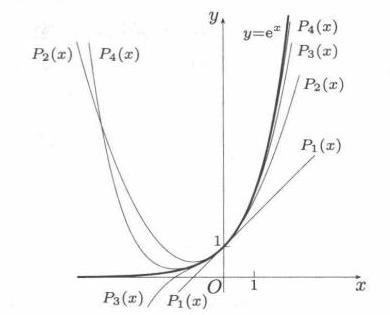
\includegraphics[width=.45\linewidth]{figures/upper/ch07/fig-7-6.png}

  图 7.6
\end{center}

我们看到，对于 $n=3,4$，Taylor 多项式在 $\abs{x}$ 不很大时已提供了对 $\ee^x$ 的较好的逼近。但是当 $\abs{x}$ 足够大时，情况完全不是如此。例如，当 $n$ 为奇数时 $P_n(x)$ 都有零点。关于 $\ee^x$ 的 Taylor 多项式的一般性结论可参看第八章的第二组参考题 4。

\subsection{例题}

当 Taylor 公式中的点 $x_0=0$ 时，由于历史原因也称为 Maclaurin 公式。在各种微积分教科书中都要介绍几个基本初等函数的 Maclaurin 公式，其中包括 $\sin x,\cos x,\arctan x,\ee^x,\ln(1+x),(1+x)^\alpha\ (\alpha\neq0)$ 等，这里不再重复。

在求以上几个基本初等函数的 Maclaurin 公式时，一般的方法是直接计算函数在点 $x=0$ 处的 $n$ 阶导数的通式，这样就可得到带 Peano 余项的 Maclaurin 公式。为了得到带 Lagrange 余项的相应公式，则需要得到 $n$ 阶导函数的表达式，这就困难得多了。在上一章中关于高阶导数的不少训练与此有关。

在本小节介绍求 Taylor（或 Maclaurin）公式的间接法，这在很多求 Taylor 公式的问题中有效，且具有很大的灵活性。实际上，$\ln(1+x)$ 和 $\arctan x$ 的 Maclaurin 公式也都可以用间接法得到。但是间接法是以若干个已知的 Taylor 公式为基础的。如果连基本的 Taylor 公式都不知道，也就不可能用间接法。

在本小节中除了 Taylor 公式的计算外，还将介绍 Taylor 公式的其他应用，特别是不能归入下一章的一些问题。

在下面有关 Taylor（或 Maclaurin）公式的计算题中，如不另作说明，则均指带 Peano 余项的公式。

\begin{xexample}[7.2.1]
计算 $f(x)=\arcsin x$ 的 Maclaurin 公式直到 $x^5$ 项。
\end{xexample}
\begin{xsolution}
\textbf{解 1}\quad 对 $f$ 求导，并利用二项式展开公式，就有
\[
  f'(x)=(1-x^2)^{-\frac12}=1+\frac12x^2+\frac38x^4+\littleo(x^5)\quad(x\to0).
\]
根据上一小节的唯一性引理和带 Peano 余项的 Taylor 公式，可见上式就是 $f'(x)$ 的 Maclaurin 公式。利用 Taylor 公式中的系数公式，就可以从上式右边的已知系数反过来求出 $f'(x)$ 在 $x=0$ 处的值和各阶导数值：
\[
  1=f'(0),\quad 0=f''(0),\quad \frac12=\frac{f'''(0)}{2},\quad 0=f^{(4)}(0),\quad \frac38=\frac{f^{(5)}(0)}{4!},\quad 0=f^{(6)}(0).
\]
这样就求出所需要的前 6 阶导数：
\[
  f'(0)=1,\quad f''(0)=0,\quad f'''(0)=1,\quad f^{(4)}(0)=0,\quad f^{(5)}(0)=9,\quad f^{(6)}(0)=0.
\]
再利用 $f(0)=0$，就得到所要的 Maclaurin 公式：
\[
  \begin{aligned}
  \arcsin x
  &=x+\frac{1}{3!}x^3+\frac{9}{5!}x^5+\littleo(x^6)\\
  &=x+\frac16x^3+\frac{3}{40}x^5+\littleo(x^6)\qquad(x\to0).
  \end{aligned}
\]
\end{xsolution}

\begin{xremark}
若将以上的解法发展一步，就可以写出 $\arcsin x$ 的一般的 Maclaurin 公式，而无须求出这个函数在 $x=0$ 处的任意阶导数值，再往前一步，我们可以提出求高阶导数的一种间接计算法：从 $f(x)=\arcsin x$ 的导函数出发，计算
\[
  \begin{aligned}
  f'(x)&=(1-x^2)^{-\frac12}\\
  &=1+\sum_{k=1}^n
  \frac{(-\frac12)(-\frac32)\cdots(-\frac12-k+1)}{k!}(-x^2)^k
  +\littleo(x^{2n+1})\\
  &=1+\sum_{k=1}^n\frac{(2k-1)!!}{2^k k!}x^{2k}+\littleo(x^{2n+1})\qquad(x\to0),
  \end{aligned}
\]
就可以对任意正整数 $k$ 得到 $f^{(2k)}(0)=0$ 和
\[
  f^{(2k+1)}(0)=(2k)!\frac{(2k-1)!!}{2^k k!}=[(2k-1)!!]^2.
\]
这就是在例题 6.2.3 已经得到的结果。

请读者试用这种新方法计算 $\arctan x$ 和 $\ln(1+x)$ 的 Maclaurin 公式和它们在 $x=0$ 处的任意阶导数值。
\end{xremark}

\begin{xsolution}
\textbf{解 2}\quad 由于 $f(x)=\arcsin x$ 是奇函数，又有 $f'(0)=1$，因此它的 Maclaurin 公式的形式如下：
\[
  \arcsin x=x+ax^3+bx^5+\littleo(x^6)\qquad(x\to0).
\]
这里只有两个系数 $a$ 和 $b$ 需要确定。利用 $\arcsin x$ 是 $\sin x$ 的反函数，又利用 $\sin x$ 的 Maclaurin 公式，就有
\[
  \begin{aligned}
  x=\sin(\arcsin x)
  &=\arcsin x-\frac16(\arcsin x)^3+\frac{1}{120}(\arcsin x)^5+\littleo(x^6)\\
  &=(x+ax^3+bx^5)-\frac16(x+ax^3)^3+\frac{1}{120}x^5+\littleo(x^6)\qquad(x\to0).
  \end{aligned}
\]
比较两边同次幂项的系数，就有方程
\[
  a-\frac16=0,\qquad b-\frac16\cdot3a+\frac{1}{120}=0.
\]
这样就可解出
\[
  a=\frac16,\qquad b=\frac{3}{40}.
\]
\end{xsolution}

\begin{xexample}[7.2.2]
计算 $f(x)=\sqrt[3]{2-\cos x}$ 的 Maclaurin 公式直到 $x^5$ 项。
\end{xexample}
\begin{xsolution}
\textbf{解 1}\quad 将根式内的表达式写成 $1+(1-\cos x)$，并利用
\[
  1-\cos x=\frac{x^2}{2}-\frac{x^4}{24}+\littleo(x^5)\qquad(x\to0),
\]
就可以计算如下：
\[
  \begin{aligned}
  f(x)&=\sqrt[3]{1+(1-\cos x)}\\
  &=1+\frac{1-\cos x}{3}-\frac{(1-\cos x)^2}{9}+\bigO((1-\cos x)^3)\\
  &=1+\left(\frac{x^2}{6}-\frac{x^4}{72}\right)-\frac{x^4}{36}+\littleo(x^5)\\
  &=1+\frac{x^2}{6}-\frac{x^4}{24}+\littleo(x^5)\qquad(x\to0).
  \end{aligned}
\]
\end{xsolution}

\begin{xsolution}
\textbf{解 2}\quad 利用 $f$ 为偶函数，因此所要求的公式的形状已可确定为
\[
  f(x)=1+ax^2+bx^4+\littleo(x^5)\qquad(x\to0).
\]
为确定 $a$ 和 $b$，只要将上式代入
\[
  [f(x)]^3=2-\cos x=1+\frac{x^2}{2}-\frac{x^4}{24}+\littleo(x^5)\qquad(x\to0),
\]
就得到关于待定系数的方程
\[
  3a=\frac12,\qquad 3b+3a^2=-\frac{1}{24}.
\]
从中解出
\[
  a=\frac16,\qquad b=-\frac{1}{24}.
\]
\end{xsolution}

\begin{xexample}[7.2.3]
计算 $f(x)=\ln\frac{\sin x}{x}$ 的 Maclaurin 公式直到 $x^6$ 项。这里 $f(x)$ 在 $x=0$ 的值用函数在该点的极限值 0 来定义。
\end{xexample}
\begin{xsolution}
从正弦函数的展开式开始，有
\[
  \sin x=x-\frac{1}{3!}x^3+\frac{1}{5!}x^5-\frac{1}{7!}x^7+\littleo(x^8)\qquad(x\to0),
\]
就有
\[
  \frac{\sin x}{x}=1-\frac{1}{3!}x^2+\frac{1}{5!}x^4-\frac{1}{7!}x^6+\littleo(x^7)\qquad(x\to0).
\]
记
\[
  y=-\frac{1}{3!}x^2+\frac{1}{5!}x^4-\frac{1}{7!}x^6+\littleo(x^7)\qquad(x\to0),
\]
则 $y=\bigO(x^2)\ (x\to0)$。然后有
\[
  \begin{aligned}
  \ln\frac{\sin x}{x}
  &=\ln(1+y)\\
  &=y-\frac12y^2+\frac13y^3+\bigO(y^4)\\
  &=\left(-\frac{1}{3!}x^2+\frac{1}{5!}x^4-\frac{1}{7!}x^6\right)
    -\frac12\left(\frac{1}{36}x^4-\frac{2}{3!5!}x^6\right)
    +\frac13\left(-\frac{1}{216}x^6\right)+\littleo(x^7)\\
  &=-\frac16x^2-\frac{1}{180}x^4-\frac{1}{2835}x^6+\littleo(x^7)\qquad(x\to0).
  \end{aligned}
\]
\end{xsolution}

\begin{xexample}[7.2.4]
设已知函数（参考图 4.1）
\[
  f(x)=
  \begin{cases}
    (1+x)^{1/x},&x\neq0,\\
    \ee,&x=0
  \end{cases}
\]
在 $x=0$ 无穷次可微，计算 $f(x)$ 的 Maclaurin 公式直到 $x^4$ 项。
\end{xexample}
\begin{xsolution}
在 $x\neq0$ 时，将函数 $f$ 写为
\[
  f(x)=\exp(\ln f(x)),
\]
然后写出
\[
  \ln f(x)=\frac{\ln(1+x)}{x}=1-\frac{x}{2}+\frac{x^2}{3}-\frac{x^3}{4}+\frac{x^4}{5}+\littleo(x^4)\qquad(x\to0).
\]
将上式右边记为 $1+y$，就有
\[
  f(x)=\ee^{1+y}=\ee\cdot\ee^y
  =\ee\left(1+y+\frac{y^2}{2!}+\frac{y^3}{3!}+\frac{y^4}{4!}\right)+\littleo(x^4)\qquad(x\to0),
\]
其中
\[
  y=-\frac{x}{2}+\frac{x^2}{3}-\frac{x^3}{4}+\frac{x^4}{5}+\littleo(x^4)\qquad(x\to0).
\]
分别计算出
\[
  y^2=\frac14x^2-\frac13x^3+\frac{13}{36}x^4+\littleo(x^4)\qquad(x\to0),
\]
\[
  y^3=-\frac18x^3+\frac14x^4+\littleo(x^4)\qquad(x\to0),
\]
\[
  y^4=\frac{1}{16}x^4+\littleo(x^4)\qquad(x\to0),
\]
代入前面的表达式中，最后得到
\[
  f(x)=\ee\left(1-\frac12x+\frac{11}{24}x^2-\frac{7}{16}x^3+\frac{2447}{5760}x^4\right)+\littleo(x^4)\qquad(x\to0).
\]
\end{xsolution}

\begin{xremark}
在上面两个例题中都没有验证函数在 $x_0=0$ 处存在任意阶导数。这是在使用间接法时经常会遇到的问题。实际上这里涉及与幂级数（或解析函数）的四则运算和复合运算有关的一些理论问题，在学幂级数之前作讨论是比较困难的。因此在例题和练习题中我们将注意力集中在计算上，而将有关的理论问题留待以后解决。此外，这里还从 $\sin x$ 和 $\ln(1+x)$ 的 Maclaurin 公式出发除以 $x$，得到函数 $\frac{\sin x}{x}$ 和 $\frac{\ln(1+x)}{x}$（在 $x=0$ 处由极限定义）的 Maclaurin 公式，这里的理论根据可在下一章得到解决（见例题 8.1.9 的第 3 个注解）。（对此有兴趣的读者还可以参考 [73] 中对于这些问题的严格处理。）
\end{xremark}

\begin{xexample}[7.2.5]
设 $f$ 在 $(0,+\infty)$ 上二阶可微，且已知
\[
  M_0=\sup\{\abs{f(x)}\mid x\in(0,+\infty)\}
\]
和
\[
  M_2=\sup\{\abs{f''(x)}\mid x\in(0,+\infty)\}
\]
为有限数。证明 $M_1=\sup\{\abs{f'(x)}\mid x\in(0,+\infty)\}$ 也是有限数，并满足不等式
\[
  M_1\leqslant2\sqrt{M_0M_2}.
\]
\end{xexample}
\begin{xproof}
写出
\[
  f(x+t)=f(x)+f'(x)t+\frac{f''(\xi)}{2}t^2,
\]
其中 $x,t>0,\ \xi\in(x,x+t)$。由此有估计
\[
  \abs{tf'(x)}\leqslant\abs{f(x+t)-f(x)-\frac{t^2}{2}f''(\xi)}
  \leqslant2M_0+\frac{t^2}{2}M_2.
\]
这样就得到
\[
  \abs{f'(x)}\leqslant\frac{2M_0}{t}+\frac{t}{2}M_2.
\]
这对每个 $x\in(0,+\infty)$ 成立。取上确界，就有
\begin{equation}
  M_1\leqslant\frac{2M_0}{t}+\frac{t}{2}M_2.
  \tag{7.24}
\end{equation}
因此 $M_1$ 为有限数。由于这对每个 $t>0$ 成立，为了得到最好的估计，可以取 $t=2\sqrt{M_0/M_2}$，使右边的和达到最小，即有
\[
  M_1\leqslant2\sqrt{M_0M_2}.
\]
\end{xproof}

\begin{xremark}
本题有许多推广和研究，例如见本章的第一组参考题 17、第二组参考题 15 等。比较详细的资料见 [30]。
\end{xremark}

\begin{xexample}[7.2.6]
设 $f$ 在 $[a,b]$ 上二阶可微。证明：存在 $\xi\in(a,b)$，使得
\[
  f(a)-2f\left(\frac{a+b}{2}\right)+f(b)=\frac14(b-a)^2f''(\xi).
\]
\end{xexample}
\begin{xproof}
写出 $f(a),f(b)$ 在点 $\frac{a+b}{2}$ 的 Taylor 展开式：
\[
  f(a)=f\left(\frac{a+b}{2}\right)
  +f'\left(\frac{a+b}{2}\right)\left(\frac{a-b}{2}\right)
  +\frac12f''(\eta_1)\left(\frac{b-a}{2}\right)^2,
\]
\[
  f(b)=f\left(\frac{a+b}{2}\right)
  +f'\left(\frac{a+b}{2}\right)\left(\frac{b-a}{2}\right)
  +\frac12f''(\eta_2)\left(\frac{b-a}{2}\right)^2,
\]
然后将两式相加，就有
\[
  f(a)-2f\left(\frac{a+b}{2}\right)+f(b)
  =\frac18(b-a)^2[f''(\eta_1)+f''(\eta_2)].
\]
对 $f''$ 用 Darboux 定理（命题 7.1.6），即有 $\xi\in(a,b)$，使得
\[
  f''(\xi)=\frac12[f''(\eta_1)+f''(\eta_2)].
\]
\end{xproof}

\begin{xremark}
本题的证明方法很多，除了用 Taylor 公式为主要工具的上述证明外，这里再简述两种证明方法：

1. 令
\[
  \lambda=\frac{f(a)+f(b)-2f\left(\frac{a+b}{2}\right)}{(b-a)^2/4},
\]
构造辅助函数
\[
  F(t)=f(t)+f(a)-2f\left(\frac{t+a}{2}\right)-\lambda\frac{(t-a)^2}{4},
\]
以下与例题 7.1.3 相同。

2. 作辅助函数
\[
  \varphi(x)=f\left(x+\frac{b-a}{2}\right)-f(x),
\]
然后考虑差 $\varphi\left(\frac{a+b}{2}\right)-\varphi(a)$。
\end{xremark}

\subsection{Euler 数与 Bernoulli 数}

在初等函数的 Taylor 展开式中有几个例子，如 $\sec x$ 和 $\tan x$，一般难以求出通式。原因在于其中出现了著名的 Euler 数和 Bernoulli 数。

\begin{xexample}[7.2.7]
计算 $\sec x$ 的 Maclaurin 展开式。
\end{xexample}
\begin{xsolution}
由于 $\sec x$ 是偶函数，可以假定有
\[
  \sec x=c_0+c_2x^2+c_4x^4+\cdots+c_{2n}x^{2n}+\littleo(x^{2n+1})\qquad(x\to0).
\]
现在令
\[
  c_{2n}=(-1)^n\frac{E_{2n}}{(2n)!},\qquad n\in\NN_+,
\]
写出
\begin{equation}
  \sec x=E_0-\frac{E_2}{2!}x^2+\frac{E_4}{4!}x^4+\cdots+(-1)^n\frac{E_{2n}}{(2n)!}x^{2n}+\littleo(x^{2n+1})\qquad(x\to0).
  \tag{7.25}
\end{equation}
将公式 (7.25) 和 $\cos x$ 的 Maclaurin 公式一起代入恒等式 $\cos x\sec x\equiv1$ 中，就可以得到确定数列 $\{E_{2n}\}$ 的递推公式：
\[
  E_0=1,\qquad E_2+E_0=0,\qquad E_4+\frac{4!}{2!2!}E_2+E_0=0,
\]
\[
  \cdots\cdots
\]
\[
  E_{2n}+\binom{2n}{2}E_{2n-2}+\binom{2n}{4}E_{2n-4}+\cdots+E_0=0.
\]
从而可以得出
\[
  E_2=-1,\quad E_4=5,\quad E_6=-61,\quad E_8=1385,\quad E_{10}=-50521,\ldots
\]
例如，这样就可以写出直到前 6 项系数的公式：
\[
  \sec x=1+\frac{x^2}{2}+\frac{5}{24}x^4+\frac{61}{720}x^6+\frac{277}{8064}x^8+\frac{50521}{3628800}x^{10}+\littleo(x^{11})\qquad(x\to0).
\]
称 $E_{2n}$ 为 \textbf{Euler 数}。当 $n$ 为偶数时，$E_{2n}$ 为正奇数，且除 $E_0$ 外，其个位数字都是 5；当 $n$ 为奇数时，$E_{2n}$ 为负奇数，其个位数字都是 1。
\end{xsolution}

\begin{xremark}
又有
\[
  \operatorname{sech}x=\frac{2}{\ee^x+\ee^{-x}}
  =E_0+\frac{E_2}{2!}x^2+\cdots+\frac{E_{2n}}{(2n)!}x^{2n}+\littleo(x^{2n+1})\qquad(x\to0),
\]
其中的函数 $\operatorname{sech}x$ 称为双曲正割。
\end{xremark}

\begin{xremark}
令 $E_{2n}=(-1)^n\overline E_n$，也有将 $\overline E_n$ 称为 Euler 数的。
\end{xremark}

Bernoulli 数是 Jacob Bernoulli 研究前 $n$ 个正整数的 $p$ 次方幂之和
\[
  1^p+2^p+3^p+\cdots+n^p
\]
的计算公式时得到的（其原文的中译文见 [35] 的 299--302 页）。对于 $p=1,2,3$ 的公式，学生在中学里都已经知道。Jacob Bernoulli 的目的是要对一切正整数 $p$ 求出一般的计算公式。他发现
\[
  \begin{aligned}
  1^p+2^p+\cdots+n^p
  ={}&\frac{1}{p+1}n^{p+1}+\frac12n^p+\frac{p}{2}An^{p-1}
  +\frac{p(p-1)(p-2)}{4!}Bn^{p-3}\\
  &+\frac{p(p-1)(p-2)(p-3)(p-4)}{6!}Cn^{p-5}+\cdots,
  \end{aligned}
\]
其中右边的项直写到 $n$ 或 $n^2$ 项为止。公式中出现的常数
\[
  A=\frac16,\qquad B=-\frac{1}{30},\qquad C=\frac{1}{42},\ldots
\]
就是 \textbf{Bernoulli 数}。

以下采用目前的标准方法来引入 Bernoulli 数。考虑计算函数
\[
  f(x)=
  \begin{cases}
    \dfrac{x}{\ee^x-1},&x\neq0,\\
    1,&x=0
  \end{cases}
\]
的 Maclaurin 展开式。令
\[
  f(x)=B_0+\frac{B_1}{1!}x+\frac{B_2}{2!}x^2+\cdots+\frac{B_n}{n!}x^n+\littleo(x^n)\qquad(x\to0),
\]
并将它代入恒等式
\[
  f(x)\cdot\frac{\ee^x-1}{x}
  =f(x)\left[1+\frac{x}{2!}+\frac{x^2}{3!}+\cdots+\frac{x^n}{(n+1)!}+\littleo(x^n)\right]\equiv1
\]
中，就可以得到确定数列 $\{B_n\}$ 的递推公式：
\[
  B_0=1,\qquad \frac{1}{2!}B_0+B_1=0,\qquad
  \frac{1}{3!}B_0+\frac{1}{2!1!}B_1+\frac{1}{2!}B_2=0,
\]
\[
  \cdots\cdots
\]
\[
  \binom n0B_0+\binom n1B_1+\binom n2B_2+\cdots+\binom n{n-1}B_{n-1}=0.
\]
从而可以得出
\[
  B_1=-\frac12,\quad B_2=\frac16,\quad B_4=-\frac{1}{30},\quad B_6=\frac{1}{42},\quad B_8=-\frac{1}{30},
\]
\[
  B_{10}=\frac{5}{66},\quad B_{12}=-\frac{691}{2730},\quad B_{14}=\frac76,\ldots,
\]
当 $n$ 为大于 1 的奇数时 $B_n=0$。

\begin{xremark}
令 $B_{2n}=(-1)^{n-1}\overline B_n\ (n\geqslant1)$，也有称 $\overline B_n$ 为 Bernoulli 数的。注意所有 $\overline B_n>0$。
\end{xremark}

\begin{xexample}[7.2.8]
计算 $x\cot x$ 的 Maclaurin 展开式，在 $x=0$ 处的函数值补充定义为 1。
\end{xexample}
\begin{xsolution}
以下运算越出了实数的范围，还用到了 Euler 公式 $\ee^{\ii x}=\cos x+\ii\sin x$，其合理性将在复变函数论中得到解释。
\[
  \begin{aligned}
  x\cot x
  &=x\cdot\frac{\cos x}{\sin x}
  =\ii x\cdot\frac{\ee^{\ii x}+\ee^{-\ii x}}{\ee^{\ii x}-\ee^{-\ii x}}
  =\ii x+\frac{2\ii x}{\ee^{2\ii x}-1}\\
  &=\ii x+B_0+\frac{B_1}{1!}2\ii x+\frac{B_2}{2!}(2\ii x)^2+\cdots+\frac{B_{2n}}{(2n)!}(2\ii x)^{2n}+\littleo(x^{2n})\\
  &=\operatorname{Re}\left[\ii x+B_0+\frac{B_1}{1!}2\ii x+\frac{B_2}{2!}(2\ii x)^2+\cdots+\frac{B_{2n}}{(2n)!}(2\ii x)^{2n}+\littleo(x^{2n})\right]\\
  &=1-\frac{\overline B_1 2^2}{2!}x^2-\frac{\overline B_2 2^4}{4!}x^4-\cdots-\frac{\overline B_n2^{2n}}{(2n)!}x^{2n}+\littleo(x^{2n+1})\qquad(x\to0).
  \end{aligned}
\]
写出其前 5 项的系数，即有
\[
  x\cot x=1-\frac13x^2-\frac{1}{45}x^4-\frac{2}{945}x^6-\frac{1}{4725}x^8+\littleo(x^9)\qquad(x\to0).
\]
\end{xsolution}

\begin{xexample}[7.2.9]
计算函数 $\tan x$ 的 Maclaurin 展开式。
\end{xexample}
\begin{xsolution}
利用恒等式 $\tan x=\cot x-2\cot2x$，当 $x=0$ 时将右边取其极限 0。这样就有
\[
  \begin{aligned}
  \tan x
  &=\frac{x\cot x-2x\cot2x}{x}\\
  &=\frac{\overline B_1(2^2-1)2^2}{2!}x
   +\frac{\overline B_2(2^4-1)2^4}{4!}x^3+\cdots\\
  &\quad+\frac{\overline B_n(2^{2n}-1)2^{2n}}{(2n)!}x^{2n-1}+\littleo(x^{2n})\qquad(x\to0).
  \end{aligned}
\]
写出其前 5 项的系数，即有
\[
  \tan x=x+\frac13x^3+\frac{2}{15}x^5+\frac{17}{315}x^7+\frac{62}{2835}x^9+\littleo(x^{10})\qquad(x\to0).
\]
\end{xsolution}

这样的例子还有很多，例如在 $x\csc x,\ln\cos x,\ln(\sin x/x)$ 的 Maclaurin 公式中都出现 Bernoulli 数。此外，Bernoulli 数还出现在以下无穷级数的求和公式中：
\begin{equation}
  \sum_{n=1}^{\infty}\frac{1}{n^{2k}}=\frac{\overline B_k}{2}\cdot\frac{(2\pi)^{2k}}{(2k)!},
  \tag{7.26}
\end{equation}
其中 $k$ 为正整数。这个公式可以从例题 7.2.8 的结果得到（见《数学译林》(1991) 第 10 期 348 页）。从第二章 2.3.2 小节的题 6 已经知道，无穷级数
\[
  1+\frac{1}{2^p}+\frac{1}{3^p}+\cdots+\frac{1}{n^p}+\cdots
\]
在 $p>1$ 时收敛。公式 (7.26) 给出了当 $p=2k$ 为偶数时的求和公式。它是 Euler 发现的。公式 (7.26) 的证明见本书下册的例题 16.2.3。

当 $k=1$ 时就可从公式 (7.26) 得到数学分析中的一个重要结果：
\[
  \sum_{n=1}^{\infty}\frac{1}{n^2}=1+\frac14+\frac19+\cdots+\frac{1}{n^2}+\cdots=\frac{\pi^2}{6}.
\]
求这个级数和就是所谓的 Basel 问题。在 Euler 之前没有人想到它的答案中会出现圆周率 $\pi$。有兴趣的读者可以从 [12] 的第九章中了解与此有关的故事。

在积分学的积分近似计算和 Stirling 公式中我们还会遇到 Bernoulli 数（见 11.3.2 和 11.4.2 小节）。

\subsection{练习题}

\begin{xexercise}[1]
计算 $x\csc x,\ \ln\cos x,\ \ln\left(\frac{\sin x}{x}\right)$ 的 Maclaurin 公式。
\end{xexercise}
\begin{xsolution}
利用本章中
\[
  x\cot x
  =1-\sum_{k=1}^N\frac{\overline B_k2^{2k}}{(2k)!}x^{2k}
  +\littleo(x^{2N})
  \qquad(x\to0)
\]
以及恒等式
\[
  \csc x=\cot\frac x2-\cot x,
\]
得到
\[
  x\csc x
  =1+\sum_{k=1}^N
  \frac{(2^{2k}-2)\overline B_k}{(2k)!}x^{2k}
  +\littleo(x^{2N}).
\]
前几项为
\[
  x\csc x
  =1+\frac{x^2}{6}+\frac{7x^4}{360}
  +\frac{31x^6}{15120}+\frac{127x^8}{604800}
  +\littleo(x^8).
\]

又由 $\frac{\dd}{\dd x}\ln\cos x=-\tan x$，并使用本章的 $\tan x$ 展开式逐项确定系数，可得
\[
  \ln\cos x
  =-\sum_{k=1}^N
  \frac{\overline B_k(2^{2k}-1)2^{2k}}
       {2k(2k)!}x^{2k}
  +\littleo(x^{2N}),
\]
即
\[
  \ln\cos x
  =-\frac{x^2}{2}-\frac{x^4}{12}-\frac{x^6}{45}
  -\frac{17x^8}{2520}+\littleo(x^8).
\]

最后，由
\[
  \frac{\dd}{\dd x}\ln\frac{\sin x}{x}
  =\cot x-\frac1x
\]
和 $x\cot x$ 的展开式，得到
\[
  \ln\frac{\sin x}{x}
  =-\sum_{k=1}^N
  \frac{\overline B_k2^{2k}}{2k(2k)!}x^{2k}
  +\littleo(x^{2N}),
\]
前几项为
\[
  \ln\frac{\sin x}{x}
  =-\frac{x^2}{6}-\frac{x^4}{180}-\frac{x^6}{2835}
  -\frac{x^8}{37800}+\littleo(x^8).
\]
这里各式均在 $x\to0$ 的意义下成立。
\end{xsolution}


\begin{xexercise}[2]
能否用 Taylor 公式作如下计算：
\[
  \lim_{x\to0}\frac{\sin x}{x}
  =\lim_{x\to0}\frac{x+\littleo(x^2)}{x}=1,
\]
\[
  \lim_{x\to0}\frac{1-\cos x}{x^2}
  =\lim_{x\to0}\frac{1-(1-\frac12x^2+\littleo(x^3))}{x^2}=\frac12,
\]
为什么？
\end{xexercise}
\begin{xsolution}
能。Taylor 公式本来就是当 $x\to x_0$ 时的局部展开；这里取 $x_0=0$，恰好满足其使用条件。

由带 Peano 余项的 Taylor 公式，
\[
  \sin x=x+\littleo(x^2)\qquad(x\to0),
\]
故对 $x\neq0$，
\[
  \frac{\sin x}{x}=1+\frac{\littleo(x^2)}x=1+\littleo(x)\to1.
\]
同理，
\[
  \cos x=1-\frac{x^2}{2}+\littleo(x^3)\qquad(x\to0),
\]
于是
\[
  \frac{1-\cos x}{x^2}
  =\frac12-\frac{\littleo(x^3)}{x^2}
  =\frac12+\littleo(x)\to\frac12.
\]
因此题中两种计算都是可以的。
\end{xsolution}


\begin{xexercise}[3]
试对函数 $f(x)=(x+a)^n\ (a\neq0)$ 和 $x_0=0$ 计算它的 Taylor 多项式，从而得到二项式展开定理的一个新证明。
\end{xexercise}
\begin{xsolution}
令 $f(x)=(x+a)^n$。对 $0\leqslant k\leqslant n$，
\[
  f^{(k)}(x)=\frac{n!}{(n-k)!}(x+a)^{n-k},
\]
故
\[
  \frac{f^{(k)}(0)}{k!}
  =\binom nk a^{n-k}.
\]
由于 $f$ 本身就是 $n$ 次多项式，它在 $x_0=0$ 的 $n$ 阶 Taylor 多项式与 $f$ 完全相同，因此
\[
  (x+a)^n
  =\sum_{k=0}^n\binom nk a^{n-k}x^k.
\]
这正是二项式展开定理。
\end{xsolution}


\begin{xexercise}[4]
设 $f$ 在 $x_0$ 处存在 $f^{(n)}(x_0)$，且有
\[
  f(x)=\sum_{k=0}^n a_k(x-x_0)^k+\littleo((x-x_0)^n)\qquad(x\to x_0),
\]
证明：
\[
  f'(x)=\sum_{k=0}^{n-1}(k+1)a_{k+1}(x-x_0)^k+\littleo((x-x_0)^{n-1})\qquad(x\to x_0).
\]
\end{xexercise}
\begin{xsolution}
不能直接把给定式中的 $\littleo$ 余项逐项求导；正确做法是利用 Taylor 系数的唯一性。

由题设展开式和命题 7.2.1，
\[
  a_k=\frac{f^{(k)}(x_0)}{k!},
  \qquad k=0,1,\ldots,n.
\]
函数 $f'$ 在 $x_0$ 存在到 $n-1$ 阶导数，且
\[
  (f')^{(k)}(x_0)=f^{(k+1)}(x_0).
\]
对 $f'$ 使用带 Peano 余项的 Taylor 公式，得到
\[
  \begin{aligned}
  f'(x)
  &=\sum_{k=0}^{n-1}\frac{f^{(k+1)}(x_0)}{k!}(x-x_0)^k
    +\littleo((x-x_0)^{n-1})\\
  &=\sum_{k=0}^{n-1}(k+1)a_{k+1}(x-x_0)^k
    +\littleo((x-x_0)^{n-1}).
  \end{aligned}
\]
\end{xsolution}


\begin{xexercise}[5]
用间接法求函数 $f(x)=\sqrt[3]{\sin x^3}$ 的带 Peano 余项的 Maclaurin 公式，要求写出直到 $x^{13}$ 项的系数，然后利用这个公式计算出函数 $f(x)$ 在点 $x=0$ 的直到 13 阶的各阶导数值。
\end{xexercise}
\begin{xsolution}
在 $x$ 充分接近 $0$ 时按实数立方根理解。写成
\[
  f(x)=x\left(\frac{\sin x^3}{x^3}\right)^{1/3}.
\]
令 $z=x^3$。由
\[
  \frac{\sin z}{z}=1-\frac{z^2}{6}+\frac{z^4}{120}+\littleo(z^4)
\]
和
\[
  (1+u)^{1/3}=1+\frac13u-\frac19u^2+\littleo(u^2),
\]
得到
\[
  \left(\frac{\sin z}{z}\right)^{1/3}
  =1-\frac{z^2}{18}-\frac{z^4}{3240}+\littleo(z^4).
\]
所以
\[
  f(x)=x-\frac{x^7}{18}-\frac{x^{13}}{3240}+\littleo(x^{13}).
\]
由 Taylor 系数唯一性，直到 $13$ 阶的导数值为
\[
  f'(0)=1,
  \qquad
  f^{(7)}(0)=-\frac{7!}{18}=-280,
  \qquad
  f^{(13)}(0)=-\frac{13!}{3240}=-1921920,
\]
而
\[
  f^{(k)}(0)=0
\]
对 $k=2,3,4,5,6,8,9,10,11,12$ 均成立；此外 $f(0)=0$。
\end{xsolution}


\begin{xexercise}[6]
计算 $\arcsin x$ 的带 Peano 余项的 Maclaurin 公式。
\end{xexercise}
\begin{xsolution}
由
\[
  (\arcsin x)'=(1-x^2)^{-1/2}
  =\sum_{k=0}^N\frac{(2k)!}{4^k(k!)^2}x^{2k}
   +\littleo(x^{2N})
\]
和 $\arcsin0=0$，逐项确定 Taylor 系数，得到对任意 $N\geqslant0$，
\[
  \boxed{
  \arcsin x
  =\sum_{k=0}^N
    \frac{(2k)!}{4^k(k!)^2(2k+1)}x^{2k+1}
   +\littleo(x^{2N+1})
  }
  \qquad(x\to0).
\]
即
\[
  \arcsin x
  =x+\frac{x^3}{6}+\frac{3x^5}{40}
   +\frac{5x^7}{112}+\frac{35x^9}{1152}+\cdots.
\]
\end{xsolution}


\begin{xexercise}[7]
计算 $f(x)=\dfrac{\arcsin x}{\sqrt{1-x^2}}$ 的带 Peano 余项的 Maclaurin 公式。
\end{xexercise}
\begin{xsolution}
直接使用两个已知的 Peano 展开式，而不对余项求导。由练习题 6，
\[
  \arcsin x
  =\sum_{k=0}^{N-1}
    \frac{\binom{2k}{k}}{4^k(2k+1)}x^{2k+1}
   +\littleo(x^{2N-1}),
\]
又由二项式展开式
\[
  \frac1{\sqrt{1-x^2}}
  =\sum_{j=0}^{N-1}\frac{\binom{2j}{j}}{4^j}x^{2j}
   +\littleo(x^{2N-2}).
\]
将两式作有限阶 Cauchy 乘积，$x^{2n-1}$ 的系数为
\[
  \sum_{k=0}^{n-1}
  \frac{\binom{2k}{k}\binom{2n-2-2k}{n-1-k}}
       {4^{n-1}(2k+1)}
  =\frac{2^{2n-1}}{n\binom{2n}{n}}.
\]
最后一个有限组合恒等式可用 Vandermonde 卷积验证；例如把
\[
  \frac{\binom{2k}{k}}{2k+1}
  =\frac{2^{2k}}{2k+1}\frac{(1/2)_k}{k!}
\]
代入后比较二项式级数
$(1-z)^{-1/2}$ 与其一个原函数的系数即可。于是
\[
  \boxed{
  \frac{\arcsin x}{\sqrt{1-x^2}}
  =\sum_{n=1}^N
    \frac{2^{2n-1}}{n\binom{2n}{n}}x^{2n-1}
  +\littleo(x^{2N-1})
  }
  \qquad(x\to0).
\]
前几项为
\[
  \frac{\arcsin x}{\sqrt{1-x^2}}
  =x+\frac23x^3+\frac{8}{15}x^5
   +\frac{16}{35}x^7+\frac{128}{315}x^9+\cdots.
\]
\end{xsolution}


\begin{xexercise}[8]
估计下列近似公式的绝对误差：
\begin{enumerate}[label=(\arabic*)]
  \item $\ee^x\approx1+x+\dfrac{x^2}{2!}+\cdots+\dfrac{x^n}{n!}$，当 $0\leqslant x\leqslant1$；
  \item $\sin x\approx x-\dfrac{x^3}{6}$，当 $\abs{x}\leqslant\dfrac12$；
  \item $\tan x\approx x+\dfrac{x^3}{3}$，当 $\abs{x}\leqslant\dfrac{1}{10}$；
  \item $\sqrt{1+x}\approx1+\dfrac{x}{2}-\dfrac{x^2}{8}$，当 $0\leqslant x\leqslant1$。
\end{enumerate}
\end{xexercise}
\begin{xsolution}
\textbf{(1)}\quad
对 $\ee^x$ 在 $0$ 作 $n$ 阶 Taylor 展开，Lagrange 余项为
\[
  R_n(x)=\frac{\ee^\xi}{(n+1)!}x^{n+1},
  \qquad0<\xi<x\leqslant1.
\]
故
\[
  \abs{R_n(x)}
  \leqslant\frac{\ee}{(n+1)!}x^{n+1}
  \leqslant\frac{\ee}{(n+1)!}.
\]
所以在 $[0,1]$ 上的统一绝对误差不超过 $\ee/(n+1)!$。

\textbf{(2)}\quad
由于 $\sin x$ 的四次 Taylor 多项式仍为 $x-x^3/6$，使用四阶展开可把余项写成
\[
  R(x)=\frac{\cos\xi}{5!}x^5,
  \qquad \xi\text{ 在 }0\text{ 与 }x\text{ 之间}.
\]
因此当 $\abs{x}\leqslant1/2$ 时
\[
  \abs{R(x)}\leqslant\frac{\abs{x}^5}{120}
  \leqslant\frac1{3840}.
\]

\textbf{(3)}\quad
$\tan x$ 的四次 Taylor 多项式仍为 $x+x^3/3$。计算
\[
  (\tan x)^{(5)}
  =16+136\tan^2x+240\tan^4x+120\tan^6x.
\]
在 $\abs{x}\leqslant1/10$ 上，$\abs{\tan x}\leqslant\tan(1/10)$，故由 Lagrange 余项
\[
  \abs{R(x)}
  \leqslant
  \frac{16+136T^2+240T^4+120T^6}{5!}\abs{x}^5,
  \qquad T=\tan\frac1{10}.
\]
特别地，统一误差满足
\[
  \abs{R(x)}
  \leqslant
  \frac{16+136T^2+240T^4+120T^6}{120\cdot10^5}
  <1.5\times10^{-6}.
\]

\textbf{(4)}\quad
令 $f(x)=\sqrt{1+x}$。有
\[
  f'''(x)=\frac{3}{8}(1+x)^{-5/2}.
\]
在 $0\leqslant x\leqslant1$ 上，$0<f'''(x)\leqslant3/8$。二阶 Taylor 公式给出
\[
  \sqrt{1+x}=1+\frac x2-\frac{x^2}{8}
  +\frac{f'''(\xi)}{3!}x^3,
\]
故
\[
  \abs{R(x)}\leqslant\frac{1}{16}x^3\leqslant\frac1{16}.
\]
\end{xsolution}


\begin{xexercise}[9]
若函数 $f$ 在某点 $x_0$ 的任意阶 Taylor 多项式均恒等于 0，是否可推出 $f(x)\equiv0$？

（参考例题 6.2.4 的结论。）
\end{xexercise}
\begin{xsolution}
不能。典型反例是
\[
  f(x)=
  \begin{cases}
    \ee^{-1/x^2},&x\neq0,\\
    0,&x=0.
  \end{cases}
\]
可归纳证明，对每个 $n\geqslant0$，当 $x\neq0$ 时 $f^{(n)}(x)$ 都是 $\ee^{-1/x^2}$ 乘以 $1/x$ 的某个多项式，而指数衰减快于任何幂次，因此
\[
  f^{(n)}(0)=0\qquad\forall n.
\]
所以 $f$ 在 $0$ 的任意阶 Taylor 多项式都恒等于零；但 $x\neq0$ 时 $f(x)>0$。故不能由所有 Taylor 多项式为零推出函数恒为零。
\end{xsolution}


\begin{xexercise}[10]
设 $f$ 在 $[-1,1]$ 上有任意阶导数，$f^{(n)}(0)=0,\ \forall n\in\NN_+$，且存在常数 $C>0$，使得对所有 $n\in\NN_+$ 和 $x\in[-1,1]$ 成立不等式 $\abs{f^{(n)}(x)}\leqslant n!C^n$。证明：$f(x)\equiv0$。
\end{xexercise}
\begin{xsolution}
按原题文字，结论不能推出。常值函数
\[
  f(x)\equiv1
\]
在 $[-1,1]$ 上有任意阶导数，满足
\[
  f^{(n)}(0)=0\quad(n\in\NN_+),
  \qquad
  \abs{f^{(n)}(x)}=0\leqslant n!C^n,
\]
但显然 $f\not\equiv0$。

若补充条件 $f(0)=0$，则原结论成立。事实上，取
\[
  r=\min\left\{1,\frac1{2C}\right\}.
\]
对任意 $\abs{x}<r$ 和正整数 $n$，在 $0$ 处作 $n-1$ 阶 Taylor 展开。由于
\[
  f(0)=f'(0)=\cdots=f^{(n-1)}(0)=0,
\]
存在位于 $0$ 与 $x$ 之间的 $\xi$ 使
\[
  f(x)=\frac{f^{(n)}(\xi)}{n!}x^n,
\]
从而
\[
  \abs{f(x)}\leqslant(C\abs{x})^n\leqslant2^{-n}.
\]
令 $n\to\infty$ 得 $f(x)=0$，所以 $f$ 在 $0$ 的一个邻域恒为零。设 $J\subset[-1,1]$ 是包含 $0$ 且使 $f$ 恒为零的最大区间。

若 $J$ 的右端点为 $b<1$，则 $f$ 在 $b$ 左侧恒为零且有任意阶导数，连续性依次给出
\[
  f^{(k)}(b)=0,\qquad k=0,1,2,\ldots.
\]
以 $b$ 为展开点重复上述估计，又可把零区间向右延长一个固定的正长度，与 $b$ 为右端点矛盾。因此零区间一直延伸到 $1$；向左同理。故在补充 $f(0)=0$ 后确有 $f\equiv0$。
\end{xsolution}


\begin{xexercise}[11]
设 $f$ 在 $[a,b]$ 上二阶可微，且 $f'(a)=f'(b)=0$。证明：存在 $\xi\in(a,b)$，使得成立
\[
  \abs{f''(\xi)}\geqslant\frac{4}{(b-a)^2}\abs{f(b)-f(a)}.
\]
\end{xexercise}
\begin{xsolution}
记中点 $c=(a+b)/2$，并令 $D=f(b)-f(a)$。由三角不等式，
\[
  \abs{D}
  \leqslant\abs{f(c)-f(a)}+\abs{f(b)-f(c)},
\]
故两项中至少有一项不小于 $\abs D/2$。

若
\[
  \abs{f(c)-f(a)}\geqslant\frac{\abs D}{2},
\]
则在 $a$ 处用一阶 Taylor 公式，因 $f'(a)=0$，存在 $\xi\in(a,c)$ 使
\[
  f(c)-f(a)=\frac12f''(\xi)(c-a)^2
  =\frac{(b-a)^2}{8}f''(\xi).
\]
于是
\[
  \abs{f''(\xi)}
  \geqslant\frac{4\abs D}{(b-a)^2}.
\]
若较大的是 $\abs{f(b)-f(c)}$，则在 $b$ 处向左作同样的 Taylor 展开，并用 $f'(b)=0$，得到相同结论。
\end{xsolution}


\begin{xexercise}[12]
\begin{enumerate}[label=(\arabic*)]
  \item 设 $f$ 在 $(a,b)$ 上可微。试问对每个点 $\xi\in(a,b)$，是否一定存在两个点 $x_1,x_2\in(a,b)$，使得
  \[
    \frac{f(x_2)-f(x_1)}{x_2-x_1}=f'(\xi)?
  \]
  \item 设 $f$ 在 $(a,b)$ 上可微，且在某点 $\xi\in(a,b)$ 处有 $f''(\xi)>0$。证明：存在两个点 $x_1,x_2\in(a,b)$，使得成立
  \[
    \frac{f(x_2)-f(x_1)}{x_2-x_1}=f'(\xi).
  \]
\end{enumerate}
\end{xexercise}
\begin{xsolution}
\textbf{(1)}\quad
不一定。取 $f(x)=x^3$，区间取 $(-1,1)$，并令 $\xi=0$。此时 $f'(0)=0$。但对任意两个不同点 $x_1,x_2$，
\[
  \frac{f(x_2)-f(x_1)}{x_2-x_1}
  =x_1^2+x_1x_2+x_2^2.
\]
而
\[
  x_1^2+x_1x_2+x_2^2
  =\left(x_1+\frac{x_2}{2}\right)^2+\frac34x_2^2>0
\]
除非 $x_1=x_2=0$。因此不存在两个不同点使该割线斜率等于 $f'(0)=0$。

\textbf{(2)}\quad
令
\[
  g(x)=f(x)-f'(\xi)x.
\]
则 $g'(\xi)=0$，且 $g''(\xi)=f''(\xi)>0$。由二阶导数定义，存在足够小的 $\delta>0$，使
\[
  g'(x)<0\quad(\xi-\delta<x<\xi),
  \qquad
  g'(x)>0\quad(\xi<x<\xi+\delta).
\]
所以 $g$ 在 $\xi$ 左侧严格下降、右侧严格上升，$\xi$ 是该小邻域中的严格最小值点。

取一个数
\[
  y\in\bigl(g(\xi),\min\{g(\xi-\delta),g(\xi+\delta)\}\bigr).
\]
由连续性，分别存在
\[
  x_1\in(\xi-\delta,\xi),
  \qquad
  x_2\in(\xi,\xi+\delta)
\]
使 $g(x_1)=g(x_2)=y$。于是
\[
  f(x_2)-f(x_1)=f'(\xi)(x_2-x_1),
\]
即
\[
  \frac{f(x_2)-f(x_1)}{x_2-x_1}=f'(\xi).
\]
\end{xsolution}


\begin{xexercise}[13]
设 $f$ 在 $[a,+\infty)$ 上二阶可微，且 $f(x)\geqslant0,\ f''(x)\leqslant0$，证明：在 $x\geqslant a$ 时 $f'(x)\geqslant0$。
\end{xexercise}
\begin{xsolution}
因 $f''\leqslant0$，由 Lagrange 中值定理可知 $f'$ 单调不增。若存在 $x_0\geqslant a$ 使 $f'(x_0)<0$，则对所有 $x>x_0$ 都有
\[
  f'(x)\leqslant f'(x_0)<0.
\]
对 $[x_0,x]$ 使用 Lagrange 中值定理，存在 $\xi\in(x_0,x)$ 使
\[
  f(x)-f(x_0)=f'(\xi)(x-x_0)
  \leqslant f'(x_0)(x-x_0).
\]
右端随 $x\to+\infty$ 趋于 $-\infty$，从而 $f(x)$ 最终为负，与 $f(x)\geqslant0$ 矛盾。因此对所有 $x\geqslant a$ 都有 $f'(x)\geqslant0$。
\end{xsolution}


\begin{xexercise}[14]
设 $f$ 在 $(-1,1)$ 上 $n+1$ 阶可微，$f^{(n+1)}(0)\neq0,\ n\in\NN_+$，在 $0<\abs{x}<1$ 上有
\[
  f(x)=f(0)+f'(0)x+\cdots+\frac{f^{(n-1)}(0)}{(n-1)!}x^{n-1}+\frac{f^{(n)}(\theta x)}{n!}x^n,
\]
其中 $0<\theta<1$，证明：
\[
  \lim_{x\to0}\theta=\frac{1}{n+1}.
\]
\end{xexercise}
\begin{xsolution}
令 $A=f^{(n)}(0)$，$B=f^{(n+1)}(0)\neq0$。在 $x=0$ 处作 Taylor 展开，题中等式左边减去前 $n-1$ 项后为
\[
  \frac{A}{n!}x^n+\frac{B}{(n+1)!}x^{n+1}
  +\littleo(x^{n+1}).
\]
另一方面，
\[
  f^{(n)}(\theta x)=A+B\theta x+\littleo(x),
\]
因为 $0<\theta<1$ 保证 $\theta x\to0$。故题中余项为
\[
  \frac{A}{n!}x^n+\frac{B\theta}{n!}x^{n+1}
  +\littleo(x^{n+1}).
\]
比较 $x^{n+1}$ 阶项，得到
\[
  \frac{B}{(n+1)!}+\littleo(1)
  =\frac{B\theta}{n!}+\littleo(1).
\]
由于 $B\neq0$，令 $x\to0$ 即得
\[
  \lim_{x\to0}\theta=\frac1{n+1}.
\]
\end{xsolution}


\begin{xexercise}[15]
证明：在 $\abs{x}\leqslant1$ 时存在 $\theta\in(0,1)$，使得
\[
  \arcsin x=\frac{x}{\sqrt{1-(\theta x)^2}},
\]
且有
\[
  \lim_{x\to0}\theta=\frac{1}{\sqrt3}.
\]
\end{xexercise}
\begin{xsolution}
令 $F(t)=\arcsin t$。对 $x\neq0$，在 $0$ 与 $x$ 之间应用 Lagrange 中值定理，存在 $\theta\in(0,1)$ 使
\[
  \arcsin x-\arcsin0
  =F'(\theta x)x
  =\frac{x}{\sqrt{1-(\theta x)^2}}.
\]
$x=0$ 时等式显然成立。

为求 $\theta$ 的极限，比较两边的三阶展开：
\[
  \arcsin x=x+\frac{x^3}{6}+\littleo(x^3),
\]
而
\[
  \frac{x}{\sqrt{1-(\theta x)^2}}
  =x+\frac12\theta^2x^3+\littleo(x^3).
\]
故
\[
  \frac12\theta^2\to\frac16.
\]
因 $\theta>0$，
\[
  \lim_{x\to0}\theta=\frac1{\sqrt3}.
\]
\end{xsolution}


\begin{xexercise}[16]
设 $f$ 在 $O_\delta(x_0)$ 上 $n$ 阶可微，且 $f''(x_0)=\cdots=f^{(n-1)}(x_0)=0,\ f^{(n)}(x_0)\neq0$。证明：当 $0<\abs{h}<\delta$ 时，成立
\[
  f(x_0+h)-f(x_0)=hf'(x_0+\theta h),\qquad0<\theta<1,
\]
且成立
\[
  \lim_{h\to0}\theta=\frac{1}{n^{1/(n-1)}}.
\]
\end{xexercise}
\begin{xsolution}
题中极限公式有意义时应有 $n\geqslant2$。对 $0<\abs h<\delta$，在 $x_0$ 与 $x_0+h$ 之间应用 Lagrange 中值定理，存在 $0<\theta<1$ 使
\[
  f(x_0+h)-f(x_0)=hf'(x_0+\theta h).
\]

由
\[
  f''(x_0)=\cdots=f^{(n-1)}(x_0)=0,
  \qquad f^{(n)}(x_0)\neq0,
\]
在 $x_0$ 处作 Taylor 展开：
\[
  f(x_0+h)-f(x_0)-hf'(x_0)
  =\frac{f^{(n)}(x_0)}{n!}h^n+\littleo(h^n).
\]
同时对 $f'$ 展开，
\[
  f'(x_0+\theta h)-f'(x_0)
  =\frac{f^{(n)}(x_0)}{(n-1)!}(\theta h)^{n-1}
   +\littleo(h^{n-1}).
\]
将中值公式减去 $hf'(x_0)$ 后比较，约去 $h^n$ 与非零的 $f^{(n)}(x_0)$，得到
\[
  \frac1{n!}+\littleo(1)
  =\frac{\theta^{n-1}}{(n-1)!}+\littleo(1).
\]
因此
\[
  \theta^{n-1}\to\frac1n,
\]
且 $\theta>0$，所以
\[
  \boxed{\displaystyle
  \lim_{h\to0}\theta=\frac1{n^{1/(n-1)}}}.
\]
\end{xsolution}


\section{对于教学的建议}

\subsection{学习要点}

1. Fermat 定理看似简单，但却是求函数的极值和最值问题的理论基础。

2. 中值定理将函数在两个（可以相距很远）点上的函数值之差，也就是函数的增量，与函数在某点的导数值联系起来。从上一章我们已经知道函数的导数是一个局部性的概念，但通过中值定理，就可以用导数研究函数在大范围上的性质。用与不用中值定理是完全不一样的，读者只要对比例题 7.1.5 的两个证明，就可以明白这一点。其中第二个证明的复杂恰好衬托出中值定理的有力。

3. Taylor 公式是一元微分学的顶峰。公式表面上似乎复杂，但它所面对的问题却是重要的实际问题。这就是如何用多项式来逼近函数。这里只需要加、减、乘三种运算。实际上从中学开始就清楚，除了多项式以及开平方等运算之外，一般初等函数的计算都不可能直接手算，而是一定要用某些工具，如数学用表、计算器或计算机，才能实现。所有函数计算，在计算机中总是归结为多项式计算，而 Taylor 公式就是这些计算的基础。

4. 两个带有不同余项形式的 Taylor 公式（即命题 7.2.2 和 7.2.3），分别是上一章的无穷小增量公式和本章的 Lagrange 中值定理（即有限增量公式）的推广。注意它们分别代表了在微分学中两种基本的思想方法。前者注重于当 $x\to x_0$ 时余项作为无穷小量的阶的估计，后者则要将余项用高阶导数表示出来（尽管其中仍有不确定的中值）。

5. 仅仅从所得到的结果就不难看出，在多次应用中值定理的基础上所得到的 Taylor 公式大大扩展了我们对可微函数的把握和使用。这两个公式当然有极其广泛的应用。本章的训练只是为理解公式本身而安排的。

6. 在教材 [8] 的第一册第 230 页中作者有一段关于 Taylor 定理的评价，写得很出色。我们原封不动地引在下面：

“我们不想把话说得太绝对，但至少可以说：凡是用一元微分学中的定理、技巧能解决的问题，其中的大部分都可以用 Taylor 定理来解决。掌握了 Taylor 定理之后，回过头去看前面的那些理论，似乎一切都在你的掌握之中，使你有一种‘会当凌绝顶，一览众山小’的意境。从这个意义上说 ‘Taylor 定理是一元微分学的顶峰’，并不过分。”

7. \textbf{对习题课的建议}\quad 中值定理的基础是 Fermat 定理与 Rolle 定理，包括它们的证明思想。这在 §7.1 中已作了比较多的说明。如何根据具体情况使用这些有力的工具，例如什么时候用 Lagrange 余项，什么时候用 Peano 余项等，这应该作为习题课训练的一个重点。

应用中值定理的另一个难点是作适当的辅助函数，这也能体现一个学生的数学综合能力。第一组参考题 4 是个很有启发性的题，讲解此题后可进一步介绍下一个题。

\begin{xexample}[7.3.1]
设 $f$ 在 $[a,b]$ 上存在 $n+1$ 阶导数，且满足
\[
  f^{(k)}(a)=f^{(k)}(b)=0,\qquad k=0,1,2,\ldots,n,
\]
其中 $f^{(0)}(a)=f(a),\ f^{(0)}(b)=f(b)$。证明：存在 $\xi\in(a,b)$，使 $f(\xi)=f^{(n+1)}(\xi)$。
\end{xexample}
\begin{xproof}
(1) 当 $n=0$ 时，令 $h(x)=\ee^{-x}f(x)$，则
\[
  h'(x)=\ee^{-x}[f'(x)-f(x)].
\]
由于 $h(a)=h(b)=0$，故由 Rolle 定理，存在 $\xi\in(a,b)$，使得 $h'(\xi)=\ee^{-\xi}[f'(\xi)-f(\xi)]=0$。由于 $\ee^{-\xi}>0$，从而 $f(\xi)=f'(\xi)$。

(2) 当 $n>0$ 时，令 $g(x)=\sum_{k=0}^n f^{(k)}(x)$，则 $g(a)=g(b)$，且
\[
  g(x)-g'(x)=f(x)-f^{(n+1)}(x).
\]
由 (1)，存在 $\xi\in(a,b)$，使得 $g(\xi)=g'(\xi)$。即 $f(\xi)=f^{(n+1)}(\xi)$。
\end{xproof}

Taylor 展开式可以解决很多数学问题，技巧性较强。选择什么余项，在哪一点展开，是展开一点的值，还是展开多点的值进行复合都很有讲究。但在初学阶段的习题课还是要贯彻“少而精”的原则。对一般的学生而言，能用合适的余项展开 Taylor 公式就已达到基本要求。这部分内容也是考研的复习重点。我们在两组参考题中为此提供了必要的素材。

\subsection{参考题}

\paragraph{第一组参考题}

\begin{xreferenceproblem}[1]
设有 $n$ 个实数 $a_1,a_2,\ldots,a_n$ 满足
\[
  a_1-\frac13a_2+\cdots+(-1)^{n-1}\frac{a_n}{2n-1}=0,
\]
证明：方程
\[
  a_1\cos x+a_2\cos3x+\cdots+a_n\cos(2n-1)x=0
\]
在区间 $\left(0,\frac{\pi}{2}\right)$ 中至少有一个根。
\end{xreferenceproblem}
\begin{xsolution}
构造
\[
  F(x)=\sum_{k=1}^n\frac{a_k}{2k-1}\sin(2k-1)x.
\]
则 $F(0)=0$，而
\[
  F\left(\frac\pi2\right)
  =a_1-\frac13a_2+\cdots+(-1)^{n-1}\frac{a_n}{2n-1}=0.
\]
由 Rolle 定理，存在 $\xi\in(0,\pi/2)$ 使 $F'(\xi)=0$。又
\[
  F'(x)=a_1\cos x+a_2\cos3x+\cdots+a_n\cos(2n-1)x,
\]
故所给方程在 $(0,\pi/2)$ 至少有一个根。
\end{xsolution}


\begin{xreferenceproblem}[2]
设 $c\neq0$，证明：方程 $x^5+ax^4+bx^3+c=0$ 至少有两个根不是实根。
\end{xreferenceproblem}
\begin{xsolution}
设方程的五个复根按重数计为 $r_1,\ldots,r_5$。因为常数项 $c\neq0$，所有 $r_i\neq0$。若五个根全为实数，令 $y_i=1/r_i$。

由 Vieta 公式，原多项式中 $x^2$、$x$ 的系数都为零，所以根的基本对称式满足
\[
  e_3(r_1,\ldots,r_5)=0,
  \qquad
  e_4(r_1,\ldots,r_5)=0.
\]
又 $e_5=r_1\cdots r_5\neq0$，于是
\[
  \sum_{i=1}^5y_i=\frac{e_4}{e_5}=0,
  \qquad
  \sum_{1\leqslant i<j\leqslant5}y_iy_j=\frac{e_3}{e_5}=0.
\]
因此
\[
  0=\left(\sum_{i=1}^5y_i\right)^2
  =\sum_{i=1}^5y_i^2+2\sum_{i<j}y_iy_j
  =\sum_{i=1}^5y_i^2.
\]
若 $y_i$ 都为实数，这迫使 $y_i=0$，矛盾。故不可能五根全为实数。因系数均为实数，非实根成共轭对出现，所以至少有两个根不是实根。
\end{xsolution}


\begin{xreferenceproblem}[3]
设 $a\neq0$，证明：方程 $x^{2n}+a^{2n}=(x+a)^{2n}$ 只有一个实根 $x=0$。
\end{xreferenceproblem}
\begin{xsolution}
令 $t=x/a$。因 $a\neq0$，原方程等价于
\[
  t^{2n}+1=(t+1)^{2n}.
\]
设
\[
  \phi(t)=(t+1)^{2n}-t^{2n}.
\]
则
\[
  \phi'(t)=2n\bigl[(t+1)^{2n-1}-t^{2n-1}\bigr]>0
\]
对所有实数 $t$ 成立，因为奇次幂函数严格递增。因此 $\phi$ 严格递增，而 $\phi(0)=1$。方程 $\phi(t)=1$ 只有唯一解 $t=0$，即 $x=0$。
\end{xsolution}


\begin{xreferenceproblem}[4]
设 $f$ 在 $[a,b]$ 上连续，在 $(a,b)$ 上可微，且满足条件
\[
  f(a)f(b)>0,\qquad f(a)f\left(\frac{a+b}{2}\right)<0,
\]
证明：对每个实数 $k$，在 $(a,b)$ 内存在点 $\xi$，使成立 $f'(\xi)-kf(\xi)=0$。
\end{xreferenceproblem}
\begin{xsolution}
记 $m=(a+b)/2$。由
\[
  f(a)f(m)<0
\]
和连续性，在 $(a,m)$ 中存在零点 $u$。又由 $f(a)f(b)>0$ 可知 $f(b)$ 与 $f(a)$ 同号，因而 $f(m)f(b)<0$，所以在 $(m,b)$ 中存在零点 $v$。于是
\[
  a<u<m<v<b,
  \qquad f(u)=f(v)=0.
\]

任取 $k\in\RR$，令
\[
  F(x)=\ee^{-kx}f(x).
\]
则 $F(u)=F(v)=0$。Rolle 定理给出 $\xi\in(u,v)\subset(a,b)$，使
\[
  0=F'(\xi)=\ee^{-k\xi}[f'(\xi)-kf(\xi)].
\]
因指数因子非零，故 $f'(\xi)-kf(\xi)=0$。
\end{xsolution}


\begin{xreferenceproblem}[5]
设
\[
  f(x)=\sum_{k=1}^n c_k\ee^{\lambda_kx},
\]
其中 $\lambda_1,\ldots,\lambda_n$ 为互异实数，$c_1,\ldots,c_n$ 不同时为 0。证明：$f$ 的零点个数小于 $n$。
\end{xreferenceproblem}
\begin{xsolution}
只需保留非零系数项。对项数 $m$ 作归纳。$m=1$ 时函数为非零指数函数，无零点，结论成立。

设结论对 $m-1$ 项成立。对
\[
  f(x)=\sum_{j=1}^m c_j\ee^{\lambda_jx}
\]
按 $\lambda_1<\cdots<\lambda_m$ 排序，并设 $c_j\neq0$。若 $f$ 有至少 $m$ 个不同零点，则
\[
  F(x)=\ee^{-\lambda_1x}f(x)
  =c_1+\sum_{j=2}^m c_j\ee^{(\lambda_j-\lambda_1)x}
\]
也有至少 $m$ 个不同零点。连续应用 Rolle 定理一次，$F'$ 至少有 $m-1$ 个不同零点。但是
\[
  F'(x)=\sum_{j=2}^m c_j(\lambda_j-\lambda_1)
  \ee^{(\lambda_j-\lambda_1)x}
\]
是一个含 $m-1$ 个非零项、指数互异的指数多项式。按归纳假设，它的零点数应小于 $m-1$，矛盾。因此 $f$ 的不同零点数小于 $m\leqslant n$。
\end{xsolution}


\begin{xreferenceproblem}[6]
\begin{enumerate}[label=(\arabic*)]
  \item 设 $f$ 在 $[0,1]$ 上可微，$f(0)=0,\ f(x)\neq0,\ \forall x\in(0,1)$，证明：存在 $\xi\in(0,1)$，使成立
  \[
    2\frac{f'(\xi)}{f(\xi)}=\frac{f'(1-\xi)}{f(1-\xi)}.
  \]
  \item 设 $f$ 在 $[0,1]$ 上可微，$f(0)=0,\ f(x)\neq0,\ \forall x\in(0,1)$，证明：对每个 $\alpha\neq0$，存在 $\xi\in(0,1)$，使成立
  \[
    \abs{\alpha}\frac{f'(\xi)}{f(\xi)}=\frac{f'(1-\xi)}{f(1-\xi)}.
  \]
\end{enumerate}
\end{xreferenceproblem}
\begin{xsolution}
\textbf{(1)}\quad
在 $(0,1)$ 上 $f$ 不为零。定义
\[
  H(x)=f(x)^2f(1-x),\qquad0\leqslant x\leqslant1.
\]
由 $f(0)=0$，有 $H(0)=H(1)=0$。Rolle 定理给出 $\xi\in(0,1)$ 使 $H'(\xi)=0$。而
\[
  H'(x)=f(x)^2f(1-x)
  \left[2\frac{f'(x)}{f(x)}-
  \frac{f'(1-x)}{f(1-x)}\right].
\]
在 $x\in(0,1)$ 时前面的乘积不为零，所以
\[
  2\frac{f'(\xi)}{f(\xi)}
  =\frac{f'(1-\xi)}{f(1-\xi)}.
\]

\textbf{(2)}\quad
由连续性和 $f(x)\neq0$，$f$ 在 $(0,1)$ 内保持固定符号，所以 $\abs{f}$ 在该区间可微。固定 $\alpha\neq0$，设 $p=\abs\alpha>0$，定义
\[
  H(x)=\abs{f(x)}^p\abs{f(1-x)},\qquad0<x<1.
\]
有 $H(x)>0$，且由 $f(0)=0$ 可知
\[
  H(x)\to0\quad(x\to0+),
  \qquad
  H(x)\to0\quad(x\to1-).
\]
因此 $H$ 在 $(0,1)$ 某内点 $\xi$ 取得正最大值，于是 $H'(\xi)=0$。对数求导得到
\[
  p\frac{f'(\xi)}{f(\xi)}
  -\frac{f'(1-\xi)}{f(1-\xi)}=0.
\]
即
\[
  \abs\alpha\frac{f'(\xi)}{f(\xi)}
  =\frac{f'(1-\xi)}{f(1-\xi)}.
\]
\end{xsolution}


\begin{xreferenceproblem}[7]
设 $f$ 在 $[a,b]$ 上连续，在 $(a,b)$ 上可微，但不是线性函数，证明：存在 $\xi,\eta\in(a,b)$，使成立
\[
  f'(\xi)>\frac{f(b)-f(a)}{b-a}>f'(\eta).
\]
\end{xreferenceproblem}
\begin{xsolution}
记割线斜率
\[
  m=\frac{f(b)-f(a)}{b-a},
\]
并令
\[
  g(x)=f(x)-f(a)-m(x-a).
\]
则 $g(a)=g(b)=0$。因 $f$ 不是线性函数，$g$ 不恒为零，故存在 $c\in(a,b)$ 使 $g(c)\neq0$。

若 $g(c)>0$，在 $[a,c]$ 与 $[c,b]$ 上分别应用 Lagrange 中值定理，得到 $\xi\in(a,c)$、$\eta\in(c,b)$，使
\[
  g'(\xi)=\frac{g(c)}{c-a}>0,
  \qquad
  g'(\eta)=\frac{-g(c)}{b-c}<0.
\]
于是
\[
  f'(\xi)>m>f'(\eta).
\]
若 $g(c)<0$，交换 $\xi,\eta$ 的角色即可得到同样形式的结论。
\end{xsolution}


\begin{xreferenceproblem}[8]
设 $f$ 在 $[a,b]$ 上二阶可微，$f(a)=f(b)=0$，且在某点 $c\in(a,b)$ 处有 $f(c)>0$，证明：存在 $\xi\in(a,b)$，使 $f''(\xi)<0$。
\end{xreferenceproblem}
\begin{xsolution}
由 $f(a)=0<f(c)$，在 $[a,c]$ 上用 Lagrange 中值定理，存在 $u\in(a,c)$ 使
\[
  f'(u)=\frac{f(c)}{c-a}>0.
\]
同理，由 $f(c)>0=f(b)$，存在 $v\in(c,b)$ 使
\[
  f'(v)=\frac{-f(c)}{b-c}<0.
\]
在 $[u,v]$ 上对 $f'$ 用 Lagrange 中值定理，存在 $\xi\in(u,v)$ 使
\[
  f''(\xi)=\frac{f'(v)-f'(u)}{v-u}<0.
\]
\end{xsolution}


\begin{xreferenceproblem}[9]
利用例题 7.1.3 的方法（或其他方法）解决以下问题：
\begin{enumerate}[label=(\arabic*)]
  \item 设 $f$ 在 $[a,b]$ 三阶可微，且有 $f(a)=f'(a)=f(b)=0$，证明：对每个 $x\in[a,b]$，存在 $\xi\in(a,b)$，使成立
  \[
    f(x)=\frac{f'''(\xi)}{3!}(x-a)^2(x-b).
  \]
  \item 设 $f$ 在 $[0,1]$ 上五阶可微，且有 $f(1/3)=f(2/3)=f(1)=f'(1)=f''(1)=0$，证明：对每个 $x\in[0,1]$，存在 $\xi\in(0,1)$，使成立
  \[
    f(x)=\frac{f^{(5)}(\xi)}{5!}\left(x-\frac13\right)\left(x-\frac23\right)(x-1)^3.
  \]
  \item 设 $f$ 在 $[a,b]$ 上三阶可微，证明：存在 $\xi\in(a,b)$，使成立
  \[
    f(b)=f(a)+\frac12(b-a)[f'(a)+f'(b)]-\frac{1}{12}(b-a)^3f'''(\xi).
  \]
  \item 设 $f$ 在 $[a,b]$ 上二阶可微，证明：对每个 $c\in(a,b)$，有 $\xi\in(a,b)$，使成立
  \[
    \frac12f''(\xi)
    =\frac{f(a)}{(a-b)(a-c)}
    +\frac{f(b)}{(b-c)(b-a)}
    +\frac{f(c)}{(c-a)(c-b)}.
  \]
\end{enumerate}
\end{xreferenceproblem}
\begin{xsolution}
\textbf{(1)}\quad
对 $x=a$ 或 $x=b$，等式左端为零，结论立即成立。以下固定 $x\in(a,b)$。令
\[
  Q(t)=(t-a)^2(t-b),
  \qquad
  \lambda=\frac{3!f(x)}{Q(x)},
\]
并构造
\[
  F(t)=f(t)-\frac{\lambda}{3!}Q(t).
\]
由题设及 $Q(a)=Q'(a)=Q(b)=0$，有
\[
  F(a)=F'(a)=F(x)=F(b)=0.
\]
也就是说，计重数共有四个零条件。连续应用 Rolle 定理三次，存在 $\xi\in(a,b)$ 使 $F'''(\xi)=0$。因为 $Q'''(t)=3!$，
\[
  0=F'''(\xi)=f'''(\xi)-\lambda.
\]
故
\[
  f(x)=\frac{f'''(\xi)}{3!}(x-a)^2(x-b).
\]

\textbf{(2)}\quad
若 $x$ 等于 $1/3,2/3,1$ 中任一点，则两边都为零。其余情形令
\[
  Q(t)=\left(t-\frac13\right)
       \left(t-\frac23\right)(t-1)^3,
  \qquad
  \lambda=\frac{5!f(x)}{Q(x)},
\]
以及
\[
  F(t)=f(t)-\frac{\lambda}{5!}Q(t).
\]
由题设，$F$ 在 $1/3,2/3$ 各有一个零，在 $1$ 有至少三重零，又有 $F(x)=0$。计重数共有六个零条件。连续应用 Rolle 定理五次，得到 $\xi\in(0,1)$ 使
\[
  F^{(5)}(\xi)=0.
\]
因为 $Q$ 是首项系数为 $1$ 的五次多项式，$Q^{(5)}=5!$，故
\[
  f^{(5)}(\xi)=\lambda.
\]
整理即得
\[
  f(x)=\frac{f^{(5)}(\xi)}{5!}
  \left(x-\frac13\right)
  \left(x-\frac23\right)(x-1)^3.
\]

\textbf{(3)}\quad
记 $L=b-a$，先取二次多项式
\[
  p(t)=f(a)+f'(a)(t-a)
  +\frac{f'(b)-f'(a)}{2L}(t-a)^2.
\]
它满足
\[
  p(a)=f(a),\quad p'(a)=f'(a),\quad p'(b)=f'(b),
\]
且
\[
  p(b)=f(a)+\frac L2[f'(a)+f'(b)].
\]
记
\[
  E=f(b)-p(b).
\]
再令
\[
  q(t)=(t-a)^2\left(t-b-\frac L2\right).
\]
则
\[
  q(a)=q'(a)=q'(b)=0,
  \qquad q(b)=-\frac{L^3}{2},
  \qquad q'''=6.
\]
构造
\[
  F(t)=f(t)-p(t)-E\frac{q(t)}{q(b)}.
\]
于是
\[
  F(a)=F'(a)=F(b)=F'(b)=0.
\]
由 Rolle 定理反复使用三次，存在 $\xi\in(a,b)$ 使 $F'''(\xi)=0$。因 $p'''=0$，
\[
  0=f'''(\xi)-E\frac{6}{-L^3/2}
  =f'''(\xi)+\frac{12E}{L^3}.
\]
故 $E=-L^3f'''(\xi)/12$。代回 $E=f(b)-p(b)$，得到
\[
  f(b)=f(a)+\frac12(b-a)[f'(a)+f'(b)]
  -\frac1{12}(b-a)^3f'''(\xi).
\]

\textbf{(4)}\quad
取经过三点 $(a,f(a)),(b,f(b)),(c,f(c))$ 的二次插值多项式
\[
  p(x)=f(a)\frac{(x-b)(x-c)}{(a-b)(a-c)}
  +f(b)\frac{(x-c)(x-a)}{(b-c)(b-a)}
  +f(c)\frac{(x-a)(x-b)}{(c-a)(c-b)}.
\]
其二次项系数为
\[
  A=\frac{f(a)}{(a-b)(a-c)}
   +\frac{f(b)}{(b-c)(b-a)}
   +\frac{f(c)}{(c-a)(c-b)}.
\]
函数 $h=f-p$ 在 $a,c,b$ 有三个不同零点。连续使用 Rolle 定理两次，存在 $\xi\in(a,b)$ 使 $h''(\xi)=0$。于是
\[
  f''(\xi)=p''(\xi)=2A,
\]
即得到题中等式。
\end{xsolution}


\begin{xreferenceproblem}[10]
设 $0<a<b$，$f$ 在 $[a,b]$ 上可微，证明：存在 $\xi\in(a,b)$，使成立
\[
  \frac{1}{a-b}
  \begin{vmatrix}
    a&b\\
    f(a)&f(b)
  \end{vmatrix}
  =f(\xi)-\xi f'(\xi).
\]
\end{xreferenceproblem}
\begin{xsolution}
因 $0<a<b$，在 $[a,b]$ 上对
\[
  F(x)=\frac{f(x)}x,
  \qquad
  G(x)=\frac1x
\]
应用 Cauchy 中值定理。存在 $\xi\in(a,b)$ 使
\[
  \frac{F(b)-F(a)}{G(b)-G(a)}
  =\frac{F'(\xi)}{G'(\xi)}.
\]
左边为
\[
  \frac{f(b)/b-f(a)/a}{1/b-1/a}
  =\frac{af(b)-bf(a)}{a-b}
  =\frac1{a-b}
  \begin{vmatrix}a&b\\ f(a)&f(b)\end{vmatrix},
\]
右边为
\[
  \frac{[xf'(x)-f(x)]/x^2}{-1/x^2}\Big|_{x=\xi}
  =f(\xi)-\xi f'(\xi).
\]
故结论成立。
\end{xsolution}


\begin{xreferenceproblem}[11]
设 $f$ 在区间 $[a,b]$ 上连续，在 $(a,b)$ 上 $n$ 次可微，设 $a=x_0<x_1<\cdots<x_n=b$，证明：存在 $\xi\in(a,b)$，使成立
\[
  \Delta=
  \begin{vmatrix}
    1&1&\cdots&1\\
    x_0&x_1&\cdots&x_n\\
    \vdots&\vdots&&\vdots\\
    x_0^{n-1}&x_1^{n-1}&\cdots&x_n^{n-1}\\
    f(x_0)&f(x_1)&\cdots&f(x_n)
  \end{vmatrix}
  =\frac{f^{(n)}(\xi)}{n!}\prod_{i>j}(x_i-x_j).
\]
\end{xreferenceproblem}
\begin{xsolution}
令 $p$ 为通过节点 $x_0,\ldots,x_n$ 的唯一一个次数不超过 $n$ 的插值多项式，并设其最高次项系数为 $A$。用 $p(x_j)=f(x_j)$ 替换行列式最后一行后，利用行列式对最后一行的线性性，低于 $n$ 次的各项都与前面某一行线性相关而不贡献，只有 $Ax^n$ 一项留下。因此
\[
  \Delta=A\prod_{i>j}(x_i-x_j).
\]

另一方面，$h=f-p$ 在 $x_0,\ldots,x_n$ 有 $n+1$ 个不同零点。反复使用 Rolle 定理 $n$ 次，存在 $\xi\in(a,b)$ 使
\[
  h^{(n)}(\xi)=0.
\]
因为 $p^{(n)}=n!A$，故
\[
  A=\frac{f^{(n)}(\xi)}{n!}.
\]
代入上一式即得
\[
  \Delta=\frac{f^{(n)}(\xi)}{n!}
  \prod_{i>j}(x_i-x_j).
\]
\end{xsolution}


\begin{xreferenceproblem}[12]
设 $f$ 在 $[a,+\infty)$ 上可微，且 $\lim_{x\to+\infty}f'(x)=\infty$，证明：$f$ 在 $[a,+\infty)$ 上非一致连续。
\end{xreferenceproblem}
\begin{xsolution}
反证 $f$ 一致连续。由 $f'(x)\to+\infty$，对每个正整数 $n$ 可取 $X_n$ 足够大，使
\[
  f'(x)>n\qquad(x\geqslant X_n).
\]
令
\[
  x_n=X_n,
  \qquad
  y_n=X_n+\frac1n.
\]
则 $\abs{x_n-y_n}=1/n\to0$。由 Lagrange 中值定理，存在 $\xi_n\in(x_n,y_n)$ 使
\[
  f(y_n)-f(x_n)=f'(\xi_n)\frac1n>1.
\]
这与一致连续性要求的 $\abs{x_n-y_n}\to0\Rightarrow\abs{f(x_n)-f(y_n)}\to0$ 矛盾。故 $f$ 非一致连续。
\end{xsolution}


\begin{xreferenceproblem}[13]
设 $f$ 在 $(0,a]$ 上可微，又存在有限极限 $\lim_{x\to0+}\sqrt{x}f'(x)$，证明：$f$ 在 $(0,a]$ 上一致连续。
\end{xreferenceproblem}
\begin{xsolution}
设
\[
  \lim_{x\to0+}\sqrt{x}\,f'(x)=L.
\]
因此可以取 $\delta\in(0,a]$ 和 $M>0$，使对 $0<x\leqslant\delta$ 有
\[
  \abs{f'(x)}\leqslant\frac{M}{\sqrt{x}}.
\]
任取 $0<x<y\leqslant\delta$。把区间按变量 $t=s^2$ 改写，或直接对 $g(s)=f(s^2)$ 应用中值定理，有
\[
  \abs{f(y)-f(x)}
  \leqslant2M\abs{\sqrt y-\sqrt x}
  \leqslant2M\sqrt{\abs{y-x}}.
\]
所以 $f$ 在 $(0,\delta]$ 一致连续，并且当 $x\to0+$ 时形成 Cauchy 值，因而存在有限极限 $f(0+)$。补定义该极限后，$f$ 在 $[0,\delta]$ 连续，故一致连续。

在 $[\delta/2,a]$ 上连续函数也一致连续。两段在重叠区间相接，因此 $f$ 在整个 $(0,a]$ 上一致连续。
\end{xsolution}


\begin{xreferenceproblem}[14]
设 $f$ 在 $[a,+\infty)$ 上可微，且 $\lim_{x\to+\infty}f'(x)=0$，证明：
\[
  \lim_{x\to+\infty}\frac{f(x)}{x}=0.
\]
\end{xreferenceproblem}
\begin{xsolution}
任给 $\varepsilon>0$，由 $f'(x)\to0$，可取 $A$ 使
\[
  \abs{f'(t)}<\varepsilon\qquad(t\geqslant A).
\]
当 $x>A$ 时，由 Lagrange 中值定理，存在 $\xi\in(A,x)$ 使
\[
  f(x)-f(A)=f'(\xi)(x-A).
\]
因此
\[
  \left|\frac{f(x)}x\right|
  \leqslant\frac{\abs{f(A)}}x
   +\varepsilon\frac{x-A}{x}
  \leqslant\frac{\abs{f(A)}}x+\varepsilon.
\]
令 $x\to+\infty$ 得上极限不超过 $\varepsilon$。由 $\varepsilon$ 任意，
\[
  \lim_{x\to+\infty}\frac{f(x)}x=0.
\]
\end{xsolution}


\begin{xreferenceproblem}[15]
对分别满足以下两个条件的 $f$，设已知 $f(1)=1$，求 $f(2)$：
\begin{enumerate}[label=(\arabic*)]
  \item $xf'(x)+f(x)=0,\ \forall x>0$；
  \item $xf'(x)-f(x)=0,\ \forall x>0$。
\end{enumerate}
\end{xreferenceproblem}
\begin{xsolution}
\textbf{(1)}\quad
条件等价于
\[
  [xf(x)]'=xf'(x)+f(x)=0.
\]
故 $xf(x)$ 为常数。由 $f(1)=1$，该常数为 $1$，所以
\[
  f(x)=\frac1x,
  \qquad f(2)=\frac12.
\]

\textbf{(2)}\quad
有
\[
  \left(\frac{f(x)}x\right)'
  =\frac{xf'(x)-f(x)}{x^2}=0.
\]
所以 $f(x)/x$ 为常数。由 $f(1)=1$，得到 $f(x)=x$，故
\[
  f(2)=2.
\]
\end{xsolution}


\begin{xreferenceproblem}[16]
设 $f$ 在 $[0,2]$ 上二阶可微，且 $\abs{f(x)}\leqslant1,\ \abs{f''(x)}\leqslant1$，证明：$\abs{f'(x)}\leqslant2$。
\end{xreferenceproblem}
\begin{xsolution}
固定 $x\in[0,2]$。在 $x$ 向右展开到 $2$，存在 $\xi_1$ 位于 $x,2$ 之间，使
\[
  f(2)=f(x)+f'(x)(2-x)+\frac12f''(\xi_1)(2-x)^2.
\]
向左展开到 $0$，存在 $\xi_2$ 位于 $0,x$ 之间，使
\[
  f(0)=f(x)-xf'(x)+\frac12f''(\xi_2)x^2.
\]
两式相减，
\[
  2f'(x)=f(2)-f(0)
  -\frac12f''(\xi_1)(2-x)^2
  +\frac12f''(\xi_2)x^2.
\]
于是
\[
  2\abs{f'(x)}
  \leqslant2+\frac12[(2-x)^2+x^2].
\]
在 $0\leqslant x\leqslant2$ 时
\[
  (2-x)^2+x^2\leqslant4,
\]
所以 $2\abs{f'(x)}\leqslant4$，即 $\abs{f'(x)}\leqslant2$。
\end{xsolution}


\begin{xreferenceproblem}[17]
证明：若在例题 7.2.5 中的区间从 $(0,+\infty)$ 改为 $(-\infty,+\infty)$，则可以得到更好的估计 $M_1\leqslant\sqrt{2M_0M_2}$。
\end{xreferenceproblem}
\begin{xsolution}
设
\[
  M_0=\sup_{x\in\RR}\abs{f(x)},
  \qquad
  M_2=\sup_{x\in\RR}\abs{f''(x)}.
\]
若 $M_2=0$，则 $f$ 为线性函数；又因 $f$ 有界，只能是常值函数，结论显然。

设 $M_2>0$。对任意 $x\in\RR$、$t>0$，分别把 $f(x+t)$ 和 $f(x-t)$ 在 $x$ 展开到二阶：
\[
  f(x+t)=f(x)+tf'(x)+\frac12t^2f''(\xi_1),
\]
\[
  f(x-t)=f(x)-tf'(x)+\frac12t^2f''(\xi_2).
\]
相减得
\[
  2t f'(x)=f(x+t)-f(x-t)
  -\frac12t^2[f''(\xi_1)-f''(\xi_2)].
\]
于是
\[
  \abs{f'(x)}\leqslant\frac{M_0}{t}+\frac{M_2t}{2}.
\]
对 $x$ 取上确界，
\[
  M_1\leqslant\frac{M_0}{t}+\frac{M_2t}{2}.
\]
取
\[
  t=\sqrt{\frac{2M_0}{M_2}}
\]
（若 $M_0=0$ 则 $f\equiv0$），得到
\[
  M_1\leqslant\sqrt{2M_0M_2}.
\]
\end{xsolution}


\begin{xreferenceproblem}[18]
设当 $x\in[0,a]$ 时有 $\abs{f''(x)}\leqslant M$。又已知 $f$ 在 $(0,a)$ 中取到最大值。证明：
\[
  \abs{f'(0)}+\abs{f'(a)}\leqslant Ma.
\]
\end{xreferenceproblem}
\begin{xsolution}
设 $f$ 在 $c\in(0,a)$ 取得最大值。由 Fermat 定理，$f'(c)=0$。在 $[0,c]$ 上对 $f'$ 用 Lagrange 中值定理，存在 $\xi_1\in(0,c)$ 使
\[
  f'(c)-f'(0)=f''(\xi_1)c.
\]
故
\[
  \abs{f'(0)}\leqslant Mc.
\]
同理，在 $[c,a]$ 上存在 $\xi_2$ 使
\[
  f'(a)-f'(c)=f''(\xi_2)(a-c),
\]
从而
\[
  \abs{f'(a)}\leqslant M(a-c).
\]
相加即得
\[
  \abs{f'(0)}+\abs{f'(a)}\leqslant Ma.
\]
\end{xsolution}


\paragraph{第二组参考题}

\begin{xreferenceproblem}[1]
设 $f$ 在 $[a,b]$ 上可微，在 $(a,b)$ 上二阶可微，证明：存在 $\xi\in(a,b)$，使成立
\[
  f'(b)-f'(a)=f''(\xi)(b-a).
\]
（注意：这里没有假定 $f'\in C[a,b]$。）
\end{xreferenceproblem}
\begin{xsolution}
记
\[
  \lambda=\frac{f'(b)-f'(a)}{b-a},
  \qquad
  F(x)=f(x)-\frac{\lambda}{2}x^2.
\]
则
\[
  F'(a)=F'(b).
\]
我们证明存在 $\xi\in(a,b)$ 使 $F''(\xi)=0$。

若 $F'$ 在 $[a,b]$ 为常值函数，则 $F''\equiv0$，结论成立。否则存在 $c\in(a,b)$ 使 $F'(c)\neq F'(a)=F'(b)$。不妨设 $F'(c)>F'(a)$，并取
\[
  F'(a)<d<F'(c).
\]
导函数具有 Darboux 介值性质，所以在 $(a,c)$ 中存在 $u$、在 $(c,b)$ 中存在 $v$，使
\[
  F'(u)=F'(v)=d.
\]
由于 $F'$ 在 $[u,v]$ 连续且在 $(u,v)$ 可微，对 $F'$ 应用 Rolle 定理，存在 $\xi\in(u,v)$ 使 $F''(\xi)=0$。若 $F'(c)<F'(a)$ 同理。

因此
\[
  0=F''(\xi)=f''(\xi)-\lambda,
\]
即
\[
  f'(b)-f'(a)=f''(\xi)(b-a).
\]
这里没有使用 $f'$ 在端点附近连续。
\end{xsolution}


\begin{xreferenceproblem}[2]
设 $f$ 在 $\RR$ 上无限次可微，
\[
  f\left(\frac1n\right)=\frac{n^2}{n^2+1},
\]
计算 $f^{(k)}(0),\ \forall k\in\NN_+$。
\end{xreferenceproblem}
\begin{xsolution}
令
\[
  g(x)=\frac{1}{1+x^2}.
\]
题设可写成
\[
  f\left(\frac1n\right)=g\left(\frac1n\right),
  \qquad n\in\NN_+.
\]
设 $h=f-g$，则 $h(1/n)=0$，且这些零点趋于 $0$。由连续性，$h(0)=0$。又因原零点列 $x_n=1/n\to0$，且 $h'(0)$ 存在，
\[
  h'(0)=\lim_{x\to0}\frac{h(x)-h(0)}x=0,
\]
因为沿 $x=x_n$ 的子列差商恒为 $0$。

在相邻零点 $1/(n+1),1/n$ 之间应用 Rolle 定理，可得到 $h'$ 的一列非零零点 $y_n\to0$。继续归纳：假设 $h^{(j)}(0)=0$，并且 $h^{(j)}$ 有一列非零零点 $y_n\to0$，则由导数定义
\[
  h^{(j+1)}(0)
  =\lim_{x\to0}\frac{h^{(j)}(x)-h^{(j)}(0)}x=0
\]
（沿 $x=y_n$ 的子列极限已经是 $0$，而总极限存在）。再在相邻的 $y_n$ 之间用 Rolle 定理，得到 $h^{(j+1)}$ 的非零零点列趋于 $0$。故归纳得到
\[
  h^{(k)}(0)=0\qquad\forall k\geqslant0.
\]
所以
\[
  f^{(k)}(0)=g^{(k)}(0).
\]
而
\[
  \frac1{1+x^2}=1-x^2+x^4-x^6+\cdots
\]
在 $0$ 的任意有限阶 Taylor 展开中成立。因此
\[
  \boxed{
  f^{(2m)}(0)=(-1)^m(2m)!,\qquad
  f^{(2m+1)}(0)=0
  }
  \quad(m=0,1,2,\ldots).
\]
特别地，对题目要求的 $k\in\NN_+$，按奇偶取上述值即可。
\end{xsolution}


\begin{xreferenceproblem}[3]
证明：方程
\[
  x^{2n}-2x^{2n-1}+3x^{2n-2}-\cdots-2nx+2n+1=0
\]
无实根。
\end{xreferenceproblem}
\begin{xsolution}
记
\[
  P(x)=x^{2n}-2x^{2n-1}+3x^{2n-2}-\cdots-2nx+2n+1
  =\sum_{k=0}^{2n}(2n+1-k)(-x)^k.
\]
若 $x<0$，则 $-x>0$，所以每一项均为正，因而 $P(x)>0$。

若 $x\geqslant0$，利用有限等比和的求导公式可得
\[
  \sum_{k=0}^{m}(m+1-k)r^k
  =\frac{(m+1)-(m+2)r+r^{m+2}}{(1-r)^2}.
\]
取 $m=2n$、$r=-x$，得到
\[
  P(x)=\frac{x^{2n+2}+(2n+2)x+(2n+1)}{(1+x)^2}>0.
\]
故对所有实数 $x$ 都有 $P(x)>0$，所给方程无实根。
\end{xsolution}


\begin{xreferenceproblem}[4]
设 $f$ 在 $(-\infty,+\infty)$ 上二阶可微，且有界，证明：存在 $\xi$，使成立 $f''(\xi)=0$。
\end{xreferenceproblem}
\begin{xsolution}
反证。若 $f''$ 在 $\RR$ 上没有零点，由 Darboux 性质，$f''$ 必始终同号。

设 $f''>0$，则 $f'$ 严格递增。固定 $x_0$。若 $f'(x_0)>0$，则对 $x>x_0$ 有 $f'(x)\geqslant f'(x_0)>0$，由中值定理
\[
  f(x)-f(x_0)\geqslant f'(x_0)(x-x_0)\to+\infty,
\]
与 $f$ 有界矛盾。若 $f'(x_0)<0$，则向 $x\to-\infty$ 作同样估计也推出 $f$ 无界。若 $f'(x_0)=0$，取 $x_1>x_0$，严格递增给出 $f'(x_1)>0$，又归入第一种情形。故 $f''>0$ 不可能。

$f''<0$ 时对 $-f$ 使用上述论证也不可能。因此 $f''$ 必在某点 $\xi$ 取零值。
\end{xsolution}


\begin{xreferenceproblem}[5]
设 $f$ 在 $[a,b]$ 上可微，$f'(a)=f'(b)$，证明：存在 $\xi\in(a,b)$，使成立
\[
  f'(\xi)=\frac{f(\xi)-f(a)}{\xi-a}.
\]
\end{xreferenceproblem}
\begin{xsolution}
这是 Flett 中值定理的一种形式。定义
\[
  g(x)=
  \begin{cases}
    \dfrac{f(x)-f(a)}{x-a},&a<x\leqslant b,\\[1ex]
    f'(a),&x=a.
  \end{cases}
\]
由导数定义，$g$ 在 $a$ 连续；在 $(a,b)$ 可微。题目所求正是某个 $\xi\in(a,b)$ 满足 $g'(\xi)=0$，因为
\[
  g'(x)=\frac{(x-a)f'(x)-[f(x)-f(a)]}{(x-a)^2}.
\]

记 $c=f'(a)=f'(b)=g(a)$。若 $g(b)=g(a)$，直接对 $g$ 用 Rolle 定理即可。

若 $g(b)>g(a)$，注意
\[
  g'_-(b)
  =\frac{(b-a)f'(b)-[f(b)-f(a)]}{(b-a)^2}
  =\frac{g(a)-g(b)}{b-a}<0.
\]
因此在 $b$ 左侧充分近处有 $g(x)>g(b)$，所以 $g$ 在 $[a,b]$ 的最大值既不在 $a$（因 $g(a)<g(b)$），也不在 $b$。最大值必在某个内点 $\xi$ 取得，故 $g'(\xi)=0$。

若 $g(b)<g(a)$，则同一计算给出 $g'_-(b)>0$，所以 $b$ 左侧有 $g(x)<g(b)$；而 $g(b)<g(a)$，故最小值既不在 $a$ 也不在 $b$，必在内点取得，同样有 $g'(\xi)=0$。

于是总有
\[
  f'(\xi)=\frac{f(\xi)-f(a)}{\xi-a}.
\]
\end{xsolution}


\begin{xreferenceproblem}[6]
设 $f$ 在 $[a,b]$ 上连续，在 $(a,b)$ 上可微，又有 $c\in(a,b)$ 使成立 $f'(c)=0$，证明：存在 $\xi\in(a,b)$，满足
\[
  f'(\xi)=\frac{f(\xi)-f(a)}{b-a}.
\]
\end{xreferenceproblem}
\begin{xsolution}
记 $L=b-a>0$，并定义
\[
  H(x)=\ee^{-x/L}[f(x)-f(a)],\qquad a\leqslant x\leqslant c.
\]
则 $H(a)=0$，且
\[
  H'(x)=\ee^{-x/L}
  \left[f'(x)-\frac{f(x)-f(a)}L\right].
\]
我们要证明 $H'$ 在 $(a,c)$ 有零点。

若 $f(c)=f(a)$，则 $H(a)=H(c)=0$，Rolle 定理立即给出结论。

若 $f(c)>f(a)$，则 $H(c)>0$，而由 $f'(c)=0$，
\[
  H'(c)=-\frac{\ee^{-c/L}}L[f(c)-f(a)]<0.
\]
故 $c$ 不可能是 $H$ 在 $[a,c]$ 的最大值点；同时 $a$ 也不可能是最大值点，因为 $H(c)>H(a)$。所以最大值在某内点 $\xi\in(a,c)$ 取得，$H'(\xi)=0$。

若 $f(c)<f(a)$，则 $H(c)<0$ 且 $H'(c)>0$，同理 $H$ 的最小值在内点取得，也有 $H'(\xi)=0$。

因此存在 $\xi\in(a,c)\subset(a,b)$，满足
\[
  f'(\xi)=\frac{f(\xi)-f(a)}{b-a}.
\]
\end{xsolution}


\begin{xreferenceproblem}[7]
设 $f$ 在 $[a,b]$ 上连续，在 $(a,b)$ 上可微，$f(a)=0,\ f(x)>0,\ \forall x\in[a,b]$，证明：对每个 $\alpha>0$，存在 $x_1,x_2\in(a,b)$，使成立
\[
  \frac{f'(x_1)}{f(x_1)}=\alpha\frac{f'(x_2)}{f(x_2)}.
\]
% SOURCE-ERR: 原书确实同时印作 f(a)=0 与 f(x)>0, \forall x\in[a,b]，两条件在端点 a 处矛盾；此处忠实保留原文。
\end{xreferenceproblem}
\begin{xsolution}
题面把 $f(a)=0$ 与 $f(x)>0\ (x\in[a,b])$ 同时列出，在端点 $a$ 处相互冲突。按与端点条件相容的读法，将正性条件理解为
\[
  f(x)>0,\qquad a<x<b.
\]
于是可令
\[
  g(x)=\ln f(x),\qquad a<x<b.
\]
由 $f(a)=0$、$f$ 的连续性及内点正性，
\[
  \lim_{x\to a+}g(x)=-\infty.
\]
只需证明对每个 $\alpha>0$，存在 $x_1,x_2\in(a,b)$ 使
\[
  g'(x_1)=\alpha g'(x_2).
\]

先设 $\alpha>1$。必存在某个 $x_2\in(a,b)$ 使 $g'(x_2)>0$。否则 $g'\leqslant0$，于是 $g$ 单调不增；固定任意 $x_0\in(a,b)$，对 $a<c<x_0$ 都有 $g(x_0)\leqslant g(c)$，令 $c\to a+$ 就与 $g(c)\to-\infty$ 矛盾。取 $c\in(a,x_2)$ 充分靠近 $a$，使
\[
  \frac{g(x_2)-g(c)}{x_2-a}>\alpha g'(x_2).
\]
由 Lagrange 中值定理，存在 $d\in(c,x_2)$ 使
\[
  g'(d)=\frac{g(x_2)-g(c)}{x_2-c}
  >\frac{g(x_2)-g(c)}{x_2-a}
  >\alpha g'(x_2).
\]
导函数 $g'$ 具有 Darboux 介值性质，而
\[
  g'(d)>\alpha g'(x_2)>g'(x_2),
\]
故存在 $x_1\in(d,x_2)$ 使 $g'(x_1)=\alpha g'(x_2)$。

当 $0<\alpha<1$ 时，对 $1/\alpha>1$ 应用上面的结果，再交换所得两点的角色即可；$\alpha=1$ 时任取 $x_1=x_2\in(a,b)$。最后利用
\[
  g'(x)=\frac{f'(x)}{f(x)}
\]
即得
\[
  \frac{f'(x_1)}{f(x_1)}
  =\alpha\frac{f'(x_2)}{f(x_2)}.
\]
\end{xsolution}


\begin{xreferenceproblem}[8]
设 $f$ 在 $(-\infty,+\infty)$ 上二阶连续可微，$\abs{f(x)}\leqslant1$，且有 $[f(0)]^2+[f'(0)]^2=4$，证明：存在 $\xi$，使成立 $f(\xi)+f''(\xi)=0$。
\end{xreferenceproblem}
\begin{xsolution}
令
\[
  q(x)=f(x)+f''(x).
\]
若不存在所求点，则连续函数 $q$ 在 $\RR$ 上不为零，故保持固定符号。不妨先设 $q>0$。定义
\[
  G(x)=f(x)\sin x+f'(x)\cos x.
\]
则
\[
  G'(x)=[f(x)+f''(x)]\cos x=q(x)\cos x.
\]
在 $[-\pi/2,\pi/2]$ 上 $\cos x\geqslant0$，所以 $G$ 单调不减。于是
\[
  G\left(-\frac\pi2\right)
  \leqslant G(0)
  \leqslant G\left(\frac\pi2\right),
\]
即
\[
  -f\left(-\frac\pi2\right)
  \leqslant f'(0)
  \leqslant f\left(\frac\pi2\right).
\]
由 $\abs{f}\leqslant1$ 得 $\abs{f'(0)}\leqslant1$。若 $q<0$，$G$ 单调不增，仍得到 $\abs{f'(0)}\leqslant1$。

可是题设
\[
  [f(0)]^2+[f'(0)]^2=4,
  \qquad \abs{f(0)}\leqslant1
\]
推出 $\abs{f'(0)}\geqslant\sqrt3>1$，矛盾。因此必存在 $\xi$ 使 $q(\xi)=0$，即 $f(\xi)+f''(\xi)=0$。

\medskip
\noindent\textbf{另解}\quad
在区间 $[-2,0]$ 和 $[0,2]$ 上分别应用 Lagrange 中值定理，可取
\[
  \xi_1\in(-2,0),\qquad \xi_2\in(0,2),
\]
使
\[
  f'(\xi_1)=\frac{f(0)-f(-2)}2,
  \qquad
  f'(\xi_2)=\frac{f(2)-f(0)}2.
\]
由 $\abs{f}\leqslant1$，有 $\abs{f'(\xi_1)},\abs{f'(\xi_2)}\leqslant1$。令
\[
  H(x)=f(x)^2+f'(x)^2.
\]
则
\[
  H(\xi_1),H(\xi_2)\leqslant2,
  \qquad
  H(0)=4.
\]
所以 $H$ 在 $[\xi_1,\xi_2]$ 上的最大值必在某个内点 $\xi$ 取得，并且 $H(\xi)\geqslant4$。由 Fermat 定理，
\[
  0=H'(\xi)=2f'(\xi)[f(\xi)+f''(\xi)].
\]
又因 $\abs{f(\xi)}\leqslant1$ 且 $H(\xi)\geqslant4$，
\[
  \abs{f'(\xi)}\geqslant\sqrt3>0.
\]
因此只能有
\[
  f(\xi)+f''(\xi)=0.
\]
\end{xsolution}


\begin{xreferenceproblem}[9]
设 $f$ 在 $(-\infty,+\infty)$ 上二阶连续可微，且对所有 $x,h\in\RR$ 成立
\[
  f(x+h)-f(x)=hf'\left(x+\frac h2\right),
\]
证明：$f(x)=ax^2+bx+c$。
\end{xreferenceproblem}
\begin{xsolution}
把题设中的 $x,h$ 改写成中点形式。令 $m=x+h/2$、$t=h/2$，则
\[
  f(m+t)-f(m-t)=2t f'(m),
  \qquad\forall m,t\in\RR.
\]
对 $t$ 求导，得到
\[
  f'(m+t)+f'(m-t)=2f'(m).
\]
令 $g=f'$。对于任意 $u,v\in\RR$，取 $m=(u+v)/2$、$t=(u-v)/2$，即有
\[
  g\left(\frac{u+v}{2}\right)=\frac{g(u)+g(v)}2.
\]
$g$ 连续。令 $h(x)=g(x)-g(0)$，则 $h(0)=0$，且同样满足中点方程。取 $v=0$ 得
\[
  h\left(\frac x2\right)=\frac{h(x)}2.
\]
于是对任意 $x,y$，
\[
  h(x+y)=2h\left(\frac{x+y}{2}\right)=h(x)+h(y).
\]
故 $h$ 是连续的可加函数，只能有 $h(x)=Ax$。因此
\[
  g(x)=Ax+B,
  \qquad B=g(0).
\]
于是
\[
  \left[f(x)-\frac A2x^2-Bx\right]'=0,
\]
故存在常数 $C$ 使
\[
  f(x)=\frac A2x^2+Bx+C.
\]
重命名系数即为 $f(x)=ax^2+bx+c$。
\end{xsolution}


\begin{xreferenceproblem}[10（Schwarz 定理）]
定义广义二阶导数
\[
  f^{[2]}(x)=\lim_{h\to0+}\frac{f(x+2h)-2f(x)+f(x-2h)}{4h^2},
\]
若 $f\in C[a,b]$，同时 $f^{[2]}(x)$ 在 $(a,b)$ 上处处等于 0，证明：$f$ 为线性函数。
\end{xreferenceproblem}
\begin{xsolution}
令 $\ell$ 为连接 $(a,f(a))$、$(b,f(b))$ 的直线，并设
\[
  g(x)=f(x)-\ell(x).
\]
则 $g(a)=g(b)=0$，而线性函数的广义二阶导数为零，所以
\[
  g^{[2]}(x)=0\qquad(a<x<b).
\]
只需证明 $g\equiv0$。

设存在 $c\in(a,b)$ 使 $g(c)>0$。令
\[
  q(x)=(x-a)(b-x)>0\qquad(a<x<b).
\]
取充分小的 $\varepsilon>0$，使
\[
  G(c)=g(c)-\varepsilon q(c)>0,
\]
其中 $G=g-\varepsilon q$。有 $G(a)=G(b)=0$，故 $G$ 在某个内点 $x_0$ 取得正最大值。于是对充分小的 $h>0$，
\[
  G(x_0+2h)-2G(x_0)+G(x_0-2h)\leqslant0,
\]
所以 $G^{[2]}(x_0)\leqslant0$。然而直接计算 $q^{[2]}=-2$，从而
\[
  G^{[2]}(x_0)=g^{[2]}(x_0)-\varepsilon q^{[2]}(x_0)=2\varepsilon>0,
\]
矛盾。故 $g\leqslant0$。

若存在 $c$ 使 $g(c)<0$，改取 $G=g+\varepsilon q$，则 $G$ 在内点取得负最小值，故 $G^{[2]}\geqslant0$；但此时 $G^{[2]}=-2\varepsilon<0$，仍矛盾。因此 $g\geqslant0$。

综上 $g\equiv0$，即 $f=\ell$ 为线性函数。
\end{xsolution}


\begin{xreferenceproblem}[11（Bellman--Gronwall（贝尔曼--格郎沃尔）不等式的微分形式）]
设 $f$ 在 $[0,+\infty)$ 上可微，$f(0)=0$，且有常数 $c>0$，使成立
\[
  \abs{f'(x)}\leqslant c\abs{f(x)},\qquad \forall x\in[a,+\infty),
\]
证明：$f(x)\equiv0$。
% SOURCE-ERR: 原书确实将函数定义域印作 [0,+\infty)，而不等式量词印作 \forall x\in[a,+\infty)，题中未定义 a；此处忠实保留原文。
\end{xreferenceproblem}
\begin{xsolution}
题面中的 $a$ 未定义。按与函数定义域相符的读法，将不等式理解为
\[
  \abs{f'(x)}\leqslant c\abs{f(x)},
  \qquad x\in[0,+\infty).
\]
定义
\[
  H(x)=\ee^{-2cx}f(x)^2.
\]
则 $H(x)\geqslant0$、$H(0)=0$，并且对 $x>0$ 有
\[
  \begin{aligned}
  H'(x)
  &=2\ee^{-2cx}\bigl[f(x)f'(x)-c f(x)^2\bigr]\\
  &\leqslant2\ee^{-2cx}
    \bigl[\abs{f(x)}\abs{f'(x)}-c f(x)^2\bigr]
  \leqslant0.
  \end{aligned}
\]
所以 $H$ 在 $[0,+\infty)$ 上单调不增。于是对任意 $x\geqslant0$，
\[
  0\leqslant H(x)\leqslant H(0)=0,
\]
故 $H(x)=0$，从而 $f(x)=0$。因此
\[
  f(x)\equiv0.
\]
\end{xsolution}


\begin{xreferenceproblem}[12]
设 $f$ 在 $(-1,1)$ 上有各阶导数，且对每个 $n\geqslant0$ 有 $\abs{f^{(n)}(x)}\leqslant n!\abs{x}$，证明：$f(x)\equiv0$。
\end{xreferenceproblem}
\begin{xsolution}
题设对 $n\geqslant0$ 成立，所以在 $x=0$ 有
\[
  \abs{f^{(n)}(0)}\leqslant n!\abs0=0,
\]
即
\[
  f^{(n)}(0)=0\qquad\forall n\geqslant0.
\]
固定任意 $x\in(-1,1)$。对 $f$ 在 $0$ 作 $n$ 阶 Taylor 展开，存在 $\xi_n$ 位于 $0$ 与 $x$ 之间，使
\[
  f(x)=\frac{f^{(n+1)}(\xi_n)}{(n+1)!}x^{n+1}.
\]
由题设
\[
  \abs{f^{(n+1)}(\xi_n)}\leqslant(n+1)!\abs{\xi_n}
  \leqslant(n+1)!\abs{x},
\]
故
\[
  \abs{f(x)}\leqslant\abs{x}^{n+2}.
\]
因 $\abs{x}<1$，令 $n\to\infty$ 得 $f(x)=0$。所以 $f\equiv0$。
\end{xsolution}


\begin{xreferenceproblem}[13]
设 $f$ 在 $(-\infty,+\infty)$ 上有任意阶导数，且存在常数 $C\geqslant0$，使对所有 $n\in\NN_+$ 和 $x\in(-\infty,+\infty)$ 成立不等式 $\abs{f^{(n)}(x)}\leqslant C$，又有 $f(1/n)=0,\ \forall n\in\NN_+$ 成立，证明：$f(x)\equiv0$。
\end{xreferenceproblem}
\begin{xsolution}
由 $f(1/n)=0$ 且 $1/n\to0$，连续性给出 $f(0)=0$。在相邻零点间反复使用 Rolle 定理，可归纳得到对每个 $k\geqslant1$ 都有一列 $f^{(k)}$ 的非零零点趋于 $0$。同时利用各阶导数在 $0$ 存在：若已知 $f^{(k)}(0)=0$ 且有 $y_j\to0$、$f^{(k)}(y_j)=0$，则
\[
  f^{(k+1)}(0)
  =\lim_{x\to0}\frac{f^{(k)}(x)-f^{(k)}(0)}x=0,
\]
因为该总极限存在而沿 $y_j$ 的子列为 $0$。由此归纳得到
\[
  f^{(k)}(0)=0\qquad\forall k\geqslant0.
\]

固定任意 $x\in\RR$。在 $0$ 与 $x$ 之间作 $n$ 阶 Taylor 展开，存在 $\xi_n$ 使
\[
  f(x)=\frac{f^{(n+1)}(\xi_n)}{(n+1)!}x^{n+1}.
\]
题设给出 $\abs{f^{(n+1)}(\xi_n)}\leqslant C$，故
\[
  \abs{f(x)}\leqslant\frac{C\abs{x}^{n+1}}{(n+1)!}\to0.
\]
所以对每个实数 $x$ 都有 $f(x)=0$，即 $f\equiv0$。
\end{xsolution}


\begin{xreferenceproblem}[14]
设 $f$ 在点 $x_0$ 有 $n$ 阶导数，证明：
\[
  f^{(n)}(x_0)=\lim_{h\to0}\frac{1}{h^n}\sum_{k=0}^n(-1)^{n-k}\binom nk f(x_0+kh).
\]
\end{xreferenceproblem}
\begin{xsolution}
在 $x_0$ 处使用带 Peano 余项的 Taylor 公式：
\[
  f(x_0+kh)
  =\sum_{j=0}^n\frac{f^{(j)}(x_0)}{j!}(kh)^j
   +\littleo(h^n),
\]
其中 $k=0,1,\ldots,n$ 为有限个固定整数，所以各余项可统一记为 $\littleo(h^n)$。令
\[
  S_h=\sum_{k=0}^n(-1)^{n-k}\binom nk f(x_0+kh).
\]
代入展开式，得到
\[
  S_h=\sum_{j=0}^n\frac{f^{(j)}(x_0)}{j!}h^j
  \sum_{k=0}^n(-1)^{n-k}\binom nk k^j
  +\littleo(h^n).
\]
利用 $n$ 阶有限差分恒等式
\[
  \sum_{k=0}^n(-1)^{n-k}\binom nk k^j
  =
  \begin{cases}
    0,&0\leqslant j<n,\\
    n!,&j=n,
  \end{cases}
\]
可得
\[
  S_h=f^{(n)}(x_0)h^n+\littleo(h^n).
\]
除以 $h^n$ 并令 $h\to0$，即得
\[
  f^{(n)}(x_0)
  =\lim_{h\to0}\frac1{h^n}
   \sum_{k=0}^n(-1)^{n-k}\binom nk f(x_0+kh).
\]
\end{xsolution}


\begin{xreferenceproblem}[15]
设 $f$ 在 $(-\infty,+\infty)$ 上 $n$ 阶可微，
\[
  M_k=\sup\{\abs{f^{(k)}(x)}\mid x\in(-\infty,+\infty)\},\qquad k=0,1,\ldots,n,
\]
证明：若 $M_0,M_n$ 为有限数，则 $M_1,M_2,\ldots,M_{n-1}$ 都是有限数。
\end{xreferenceproblem}
\begin{xsolution}
$n=1$ 时无中间阶导数需要证明。设 $n\geqslant2$。固定 $x\in\RR$，对 $j=1,2,\ldots,n-1$，在 $x$ 处把 $f(x+j)$ 展开到 $n-1$ 阶：
\[
  f(x+j)-f(x)
  =\sum_{k=1}^{n-1}\frac{j^k}{k!}f^{(k)}(x)
   +\frac{j^n}{n!}f^{(n)}(\xi_{j,x}),
\]
其中 $\xi_{j,x}$ 位于 $x$ 与 $x+j$ 之间。

记未知向量
\[
  X(x)=(f'(x),f''(x),\ldots,f^{(n-1)}(x))^{\mathsf T}.
\]
上述 $n-1$ 个方程写成
\[
  AX(x)=B(x),
\]
其中
\[
  A_{jk}=\frac{j^k}{k!},\qquad1\leqslant j,k\leqslant n-1.
\]
把每一列的 $1/k!$ 提出后，$A$ 是 Vandermonde 型矩阵，行节点 $1,2,\ldots,n-1$ 互异且非零，所以 $A$ 可逆。

由 $M_0,M_n<\infty$，每个 $B_j(x)$ 都有与 $x$ 无关的界：
\[
  \abs{B_j(x)}
  \leqslant2M_0+\frac{j^n}{n!}M_n.
\]
因此
\[
  X(x)=A^{-1}B(x)
\]
的每个分量都有与 $x$ 无关的有限界。故 $M_1,\ldots,M_{n-1}$ 都有限。
\end{xsolution}


\begin{xreferenceproblem}[16]
设 $f$ 在 $[0,+\infty)$ 上 $n$ 阶可微，且存在有限极限
\[
  \lim_{x\to+\infty}f(x)\quad\text{和}\quad\lim_{x\to+\infty}f^{(n)}(x),
\]
证明：对每个 $k=1,2,\ldots,n$，成立
\[
  \lim_{x\to+\infty}f^{(k)}(x)=0.
\]
\end{xreferenceproblem}
\begin{xsolution}
先证明
\[
  \lim_{x\to+\infty}f^{(n)}(x)=0.
\]
固定 $h>0$，记 $\Delta_hF(x)=F(x+h)-F(x)$。由 Lagrange 中值定理，
\[
  \Delta_h^n f(x)
  =h\,\Delta_h^{n-1}f'(\eta_1)
  =h^2\Delta_h^{n-2}f''(\eta_2)
  =\cdots
  =h^n f^{(n)}(\xi_x),
\]
其中各中值依次落在前一步区间内部，因而最终有
\[
  \xi_x\in(x,x+nh).
\]
另一方面，有限差分展开为
\[
  \Delta_h^n f(x)
  =\sum_{j=0}^n(-1)^{n-j}\binom nj f(x+jh).
\]
于是
\[
  \sum_{j=0}^n(-1)^{n-j}\binom nj f(x+jh)
  =h^n f^{(n)}(\xi_x).
\]
当 $x\to+\infty$ 时，左边每一项 $f(x+jh)$ 都趋于同一个有限极限，所以左边趋于 $0$；而 $\xi_x\to+\infty$，故右边趋于
\[
  h^n\lim_{t\to+\infty}f^{(n)}(t).
\]
因此该极限只能为 $0$。当 $n=1$ 时结论已经证明；以下设 $n\geqslant2$，再证明其余各阶。

固定 $h=1$。对 $j=1,\ldots,n-1$，Taylor 公式给出
\[
  f(x+j)-f(x)
  =\sum_{k=1}^{n-1}\frac{j^k}{k!}f^{(k)}(x)
   +\frac{j^n}{n!}f^{(n)}(\eta_{j,x}),
\]
其中 $\eta_{j,x}\to+\infty$。当 $x\to+\infty$ 时，左边趋于 $0$，最后的余项也因 $f^{(n)}(t)\to0$ 而趋于 $0$。因此
\[
  A
  \begin{pmatrix}
  f'(x)\\ \vdots\\ f^{(n-1)}(x)
  \end{pmatrix}
  \longrightarrow0,
\]
其中 $A_{jk}=j^k/k!$ 是上一题中的可逆矩阵。乘以固定矩阵 $A^{-1}$，便有
\[
  f^{(k)}(x)\to0,
  \qquad k=1,\ldots,n-1.
\]
连同已经证明的 $k=n$，结论成立。
\end{xsolution}


\begin{xreferenceproblem}[17]
\begin{enumerate}[label=(\arabic*)]
  \item 设 $f$ 在 $[a,+\infty)$ 上二阶可微，$f''$ 有界，且存在有限极限 $\lim_{x\to+\infty}f(x)$，证明：
  \[
    \lim_{x\to+\infty}f'(x)=0.
  \]
  \item 设 $f$ 在 $[a,+\infty)$ 可微，且存在有限极限 $\lim_{x\to+\infty}f(x)$，
  \begin{enumerate}[label=(\roman*)]
    \item 举例说明 $\lim_{x\to+\infty}f'(x)=0$ 不一定成立；
    \item 证明：若 $f'$ 在 $[a,+\infty)$ 上一致连续，则一定成立 $\lim_{x\to+\infty}f'(x)=0$。
  \end{enumerate}
\end{enumerate}
\end{xreferenceproblem}
\begin{xsolution}
\textbf{(1)}\quad
设 $\abs{f''(x)}\leqslant M$。若 $M=0$，则 $f'$ 为常数，而 $f$ 有有限极限迫使该常数为 $0$。

设 $M>0$。对任意固定 $t>0$，Taylor 公式给出
\[
  f(x+t)=f(x)+tf'(x)+\frac12t^2f''(\xi),
\]
故
\[
  \abs{f'(x)}
  \leqslant\frac{\abs{f(x+t)-f(x)}}t+\frac{Mt}{2}.
\]
给定 $\varepsilon>0$，先取 $t>0$ 使 $Mt/2<\varepsilon/2$。由于 $f(x)$ 有有限极限，当 $x$ 足够大时
\[
  \frac{\abs{f(x+t)-f(x)}}t<\frac\varepsilon2.
\]
于是 $\abs{f'(x)}<\varepsilon$。故
\[
  \lim_{x\to+\infty}f'(x)=0.
\]

\textbf{(2)(i)}\quad
不一定成立。例如在 $[1,+\infty)$ 上取
\[
  f(x)=\frac{\sin x^2}{x}.
\]
则 $f(x)\to0$，但
\[
  f'(x)=2\cos x^2-\frac{\sin x^2}{x^2}
\]
没有极限，更不趋于 $0$。

\textbf{(2)(ii)}\quad
反证。若 $f'(x)$ 不趋于 $0$，则存在 $\varepsilon>0$ 和 $x_n\to+\infty$，使
\[
  \abs{f'(x_n)}\geqslant\varepsilon.
\]
由 $f'$ 在 $[a,+\infty)$ 一致连续，存在 $\delta>0$，使
\[
  \abs{x-y}<\delta
  \quad\Longrightarrow\quad
  \abs{f'(x)-f'(y)}<\frac\varepsilon2.
\]
于是对 $y\in[x_n,x_n+\delta/2]$，$f'(y)$ 与 $f'(x_n)$ 同号，且
\[
  \abs{f'(y)}\geqslant\frac\varepsilon2.
\]
由 Lagrange 中值定理，
\[
  \abs{f(x_n+\delta/2)-f(x_n)}
  \geqslant\frac{\varepsilon\delta}{4}.
\]
但 $f(x)$ 有有限极限，所以上式左边随 $n\to\infty$ 应趋于 $0$，矛盾。故 $f'(x)\to0$。
\end{xsolution}


\begin{xreferenceproblem}[18]
设 $f$ 在 $(a,b)$ 上任意阶可微，且对每个正整数 $n$ 有 $f^{(n)}(x)\geqslant0$ 和 $\abs{f(x)}\leqslant M$，证明：对每个 $x\in(a,b),\ r>0,\ x+r\in(a,b)$，成立关于导数的估计式
\[
  f^{(n)}(x)\leqslant\frac{2Mn!}{r^n},\qquad \forall n\in\NN_+.
\]
\end{xreferenceproblem}
\begin{xsolution}
固定 $x\in(a,b)$ 和 $r>0$，且 $x+r\in(a,b)$。对 $f(x+r)$ 在点 $x$ 作 $n-1$ 阶 Taylor 展开，存在 $\xi\in(x,x+r)$ 使
\[
  f(x+r)
  =f(x)+\sum_{k=1}^{n-1}\frac{f^{(k)}(x)}{k!}r^k
   +\frac{f^{(n)}(\xi)}{n!}r^n.
\]
题设给出所有正阶导数非负，且 $f^{(n+1)}\geqslant0$，所以 $f^{(n)}$ 单调不减，从而
\[
  f^{(n)}(\xi)\geqslant f^{(n)}(x).
\]
其余 Taylor 项也都非负。因此
\[
  f(x+r)-f(x)\geqslant\frac{f^{(n)}(x)}{n!}r^n.
\]
又 $\abs{f}\leqslant M$，故
\[
  f(x+r)-f(x)\leqslant\abs{f(x+r)}+\abs{f(x)}\leqslant2M.
\]
于是
\[
  f^{(n)}(x)\leqslant\frac{2Mn!}{r^n}.
\]
\end{xsolution}


\begin{xreferenceproblem}[19（Bernstein（伯恩斯坦）定理）]
设 $f$ 在 $(a,b)$ 上任意阶可微，且对每个 $n$ 成立 $f^{(n)}(x)\geqslant0$，证明：对每个 $x_0\in(a,b)$ 存在 $r>0$，使得当 $x\in[x_0-r,x_0+r]\subset(a,b)$ 时，成立
\[
  f(x)=\lim_{n\to\infty}\sum_{k=0}^n\frac{f^{(k)}(x_0)}{k!}(x-x_0)^k.
\]
\end{xreferenceproblem}
\begin{xsolution}
固定 $x_0\in(a,b)$。取 $R>0$，使
\[
  [x_0-R,x_0+R]\subset(a,b).
\]
由连续性，存在 $M>0$ 使
\[
  \abs{f(x)}\leqslant M
  \qquad(x\in[x_0-R,x_0+R]).
\]
取 $\abs{x-x_0}\leqslant R/4$。对 $f(x)$ 在 $x_0$ 作 $n$ 阶 Taylor 展开，存在 $\xi_n$ 位于 $x_0$ 与 $x$ 之间，使余项为
\[
  R_n(x)=\frac{f^{(n+1)}(\xi_n)}{(n+1)!}(x-x_0)^{n+1}.
\]
此时 $\abs{\xi_n-x_0}\leqslant R/4$，所以
\[
  \xi_n+\frac R2\in[x_0-R,x_0+R].
\]
在该局部闭区间内应用上一题的估计，取 $r=R/2$，得到
\[
  f^{(n+1)}(\xi_n)
  \leqslant\frac{2M(n+1)!}{(R/2)^{n+1}}.
\]
因此
\[
  \abs{R_n(x)}
  \leqslant2M
  \left(\frac{2\abs{x-x_0}}R\right)^{n+1}.
\]
当 $\abs{x-x_0}\leqslant R/4$ 时，括号不超过 $1/2$，故 $R_n(x)\to0$。所以在
\[
  [x_0-R/4,x_0+R/4]\subset(a,b)
\]
上成立
\[
  f(x)=\lim_{n\to\infty}
  \sum_{k=0}^n\frac{f^{(k)}(x_0)}{k!}(x-x_0)^k.
\]
取 $r=R/4$ 即得题目要求。
\end{xsolution}

